\documentclass{article}%
\usepackage[T1]{fontenc}%
\usepackage[utf8]{inputenc}%
\usepackage{lmodern}%
\usepackage{textcomp}%
\usepackage{lastpage}%
\usepackage[paper=a4paper,layout=a4paper,includehead=True,includefoot=True,margin=1in]{geometry}%
\usepackage{fancyhdr}%
\usepackage{ragged2e}%
\usepackage[hidelinks]{hyperref}%
\usepackage{float}%
\usepackage[format=plain,labelfont={bf,it},textfont=it]{caption}%
\usepackage[style=authoryear,sorting=ynt]{biblatex}%
\usepackage{graphicx}%
\usepackage{longtable}%
\usepackage{subcaption}%
%
\fancypagestyle{FirstPage}{ 
\renewcommand{\headrulewidth}{0pt}%
\renewcommand{\footrulewidth}{0pt}%
\fancyhead{ 
}%
\fancyfoot{ 
}%
\title{Evaluating Remote Sensing Products for Water Accounting\\Mindanao River Basin, Philippines}%
\author{WA+ team}%
\date{\today}%
\maketitle%
\thispagestyle{empty}
}%
\fancypagestyle{PreambleHeader}{ 
\renewcommand{\headrulewidth}{0pt}%
\renewcommand{\footrulewidth}{0pt}%
\fancyhead{ 
}%
\fancyfoot{ 
}%
\fancyhead[L]{ 
}%
\fancyhead[C]{ 
}%
\fancyhead[R]{ 
IHE
}%
\fancyfoot[L]{ 
}%
\fancyfoot[C]{ 
}%
\fancyfoot[R]{ 
\thepage
}
}%
\fancypagestyle{SectionHeader}{ 
\renewcommand{\headrulewidth}{0pt}%
\renewcommand{\footrulewidth}{0pt}%
\fancyhead{ 
}%
\fancyfoot{ 
}%
\fancyhead[L]{ 
}%
\fancyhead[C]{ 
}%
\fancyhead[R]{ 
IHE
}%
\fancyfoot[L]{ 
}%
\fancyfoot[C]{ 
}%
\fancyfoot[R]{ 
\thepage
}
}%
\addbibresource{test_report.bib}%
%
\begin{document}%
\normalsize%
\newpage%
\pagestyle{FirstPage}%
\cleardoublepage%
\clearpage%
\pagenumbering{roman}%
\setcounter{page}{1}%
\pagestyle{PreambleHeader}%
\newpage%
\tableofcontents%
\addcontentsline{toc}{section}{\contentsname}%
\cleardoublepage%
\newpage%
\listoffigures%
\addcontentsline{toc}{section}{\listfigurename}%
\cleardoublepage%
\newpage%
\listoftables%
\addcontentsline{toc}{section}{\listtablename}%
\cleardoublepage%
\clearpage%
\pagenumbering{arabic}%
\setcounter{page}{1}%
\pagestyle{SectionHeader}%
\newpage%
\RaggedRight%
\section{Introduction}%
\label{sec:Introduction}%
The Mindanao River Basin is one of the selected pilot basins for Rapid Water Accounting. It covers an area of 21,503 km2 (between 124°6’E 6°3’N and 125°27’E 8°33’N), see Figure \ref{figure:fig1}.%
\linebreak%
The catchment contains the area from the mountains of Impasug-ong in Bukidnon (known as Upper Pulangi River), Kabacan River (relabeled as Mindanao River), Lower Pulangi River and Ligawasan Marsh.%
\linebreak%


\begin{figure}[H]%
\centering%
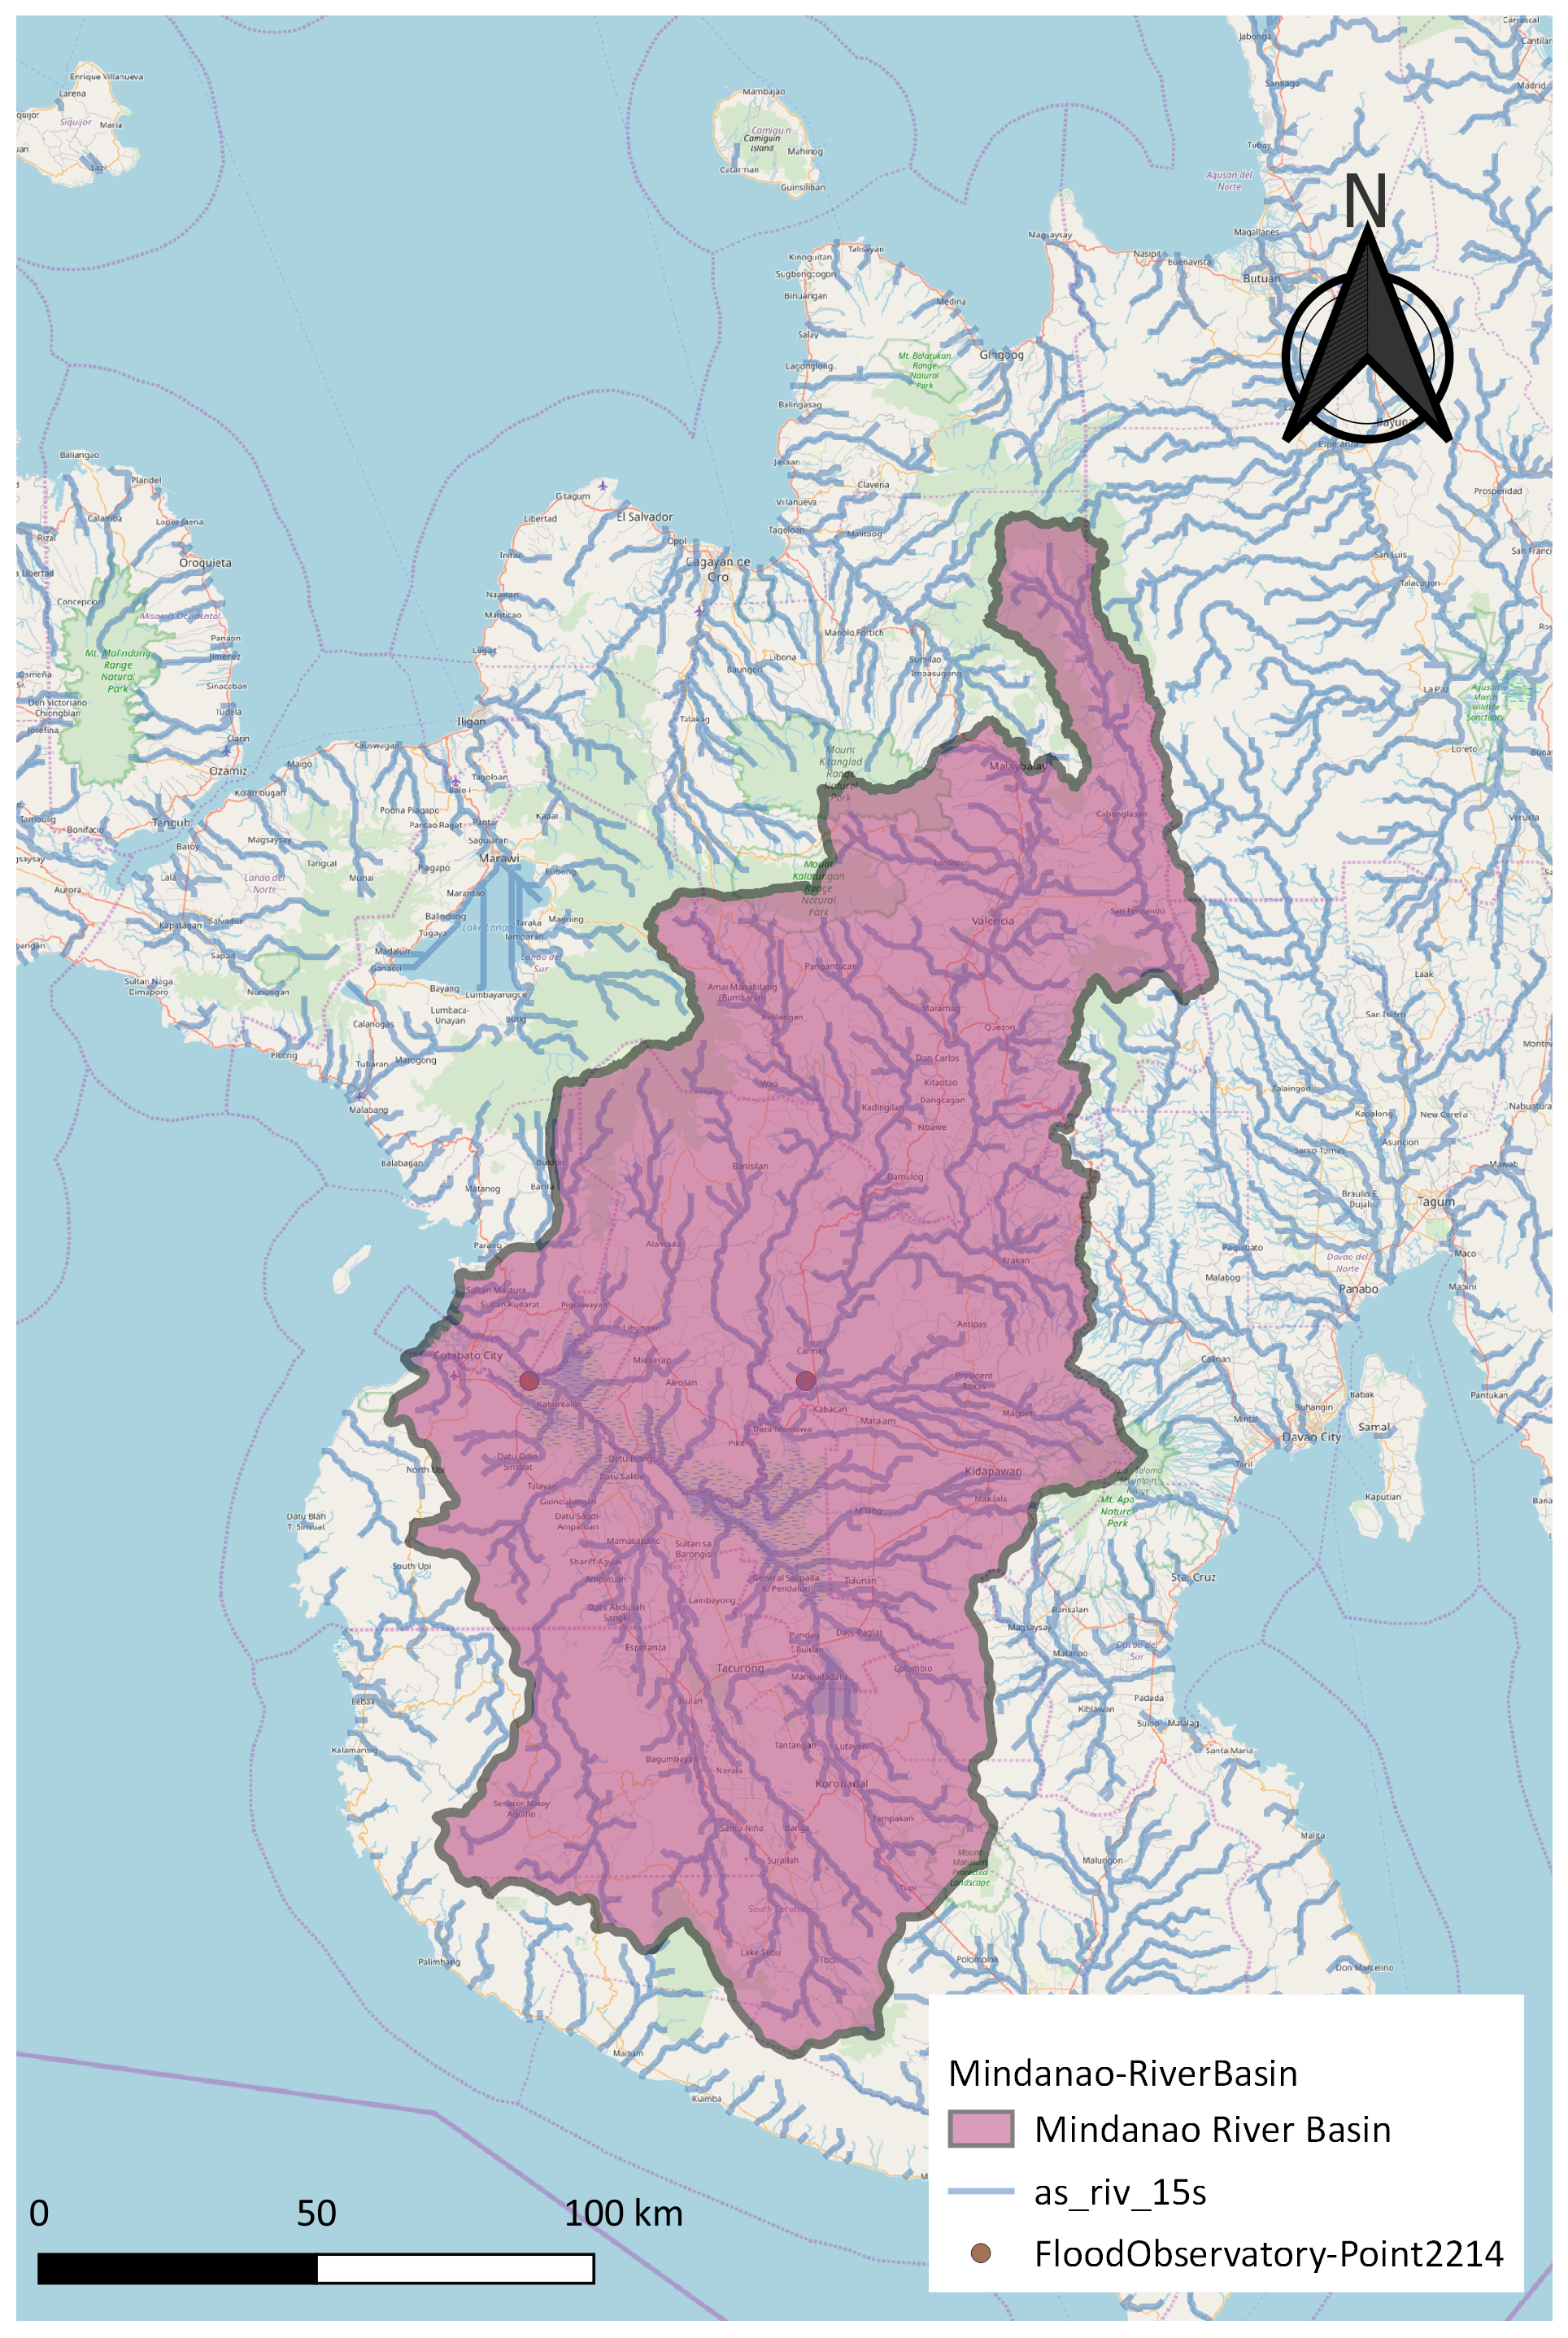
\includegraphics[width=0.6\textwidth]{D:/IHEProjects/TempDev/IHEWAreport/tests/data/area1/fig/fig1.png}%
\caption{Mindanao River Basin}%
\label{figure:fig1}%
\end{figure}

%
\subsection{Observation data}%
\label{subsec:Observationdata}%
Discharge is collected from Flood Observatory. Two flooding periods can be found, which happened in 2008 and 2011, see Figure \ref{figure:fig2}.%
\linebreak%


\begin{figure}[H]%
\centering%
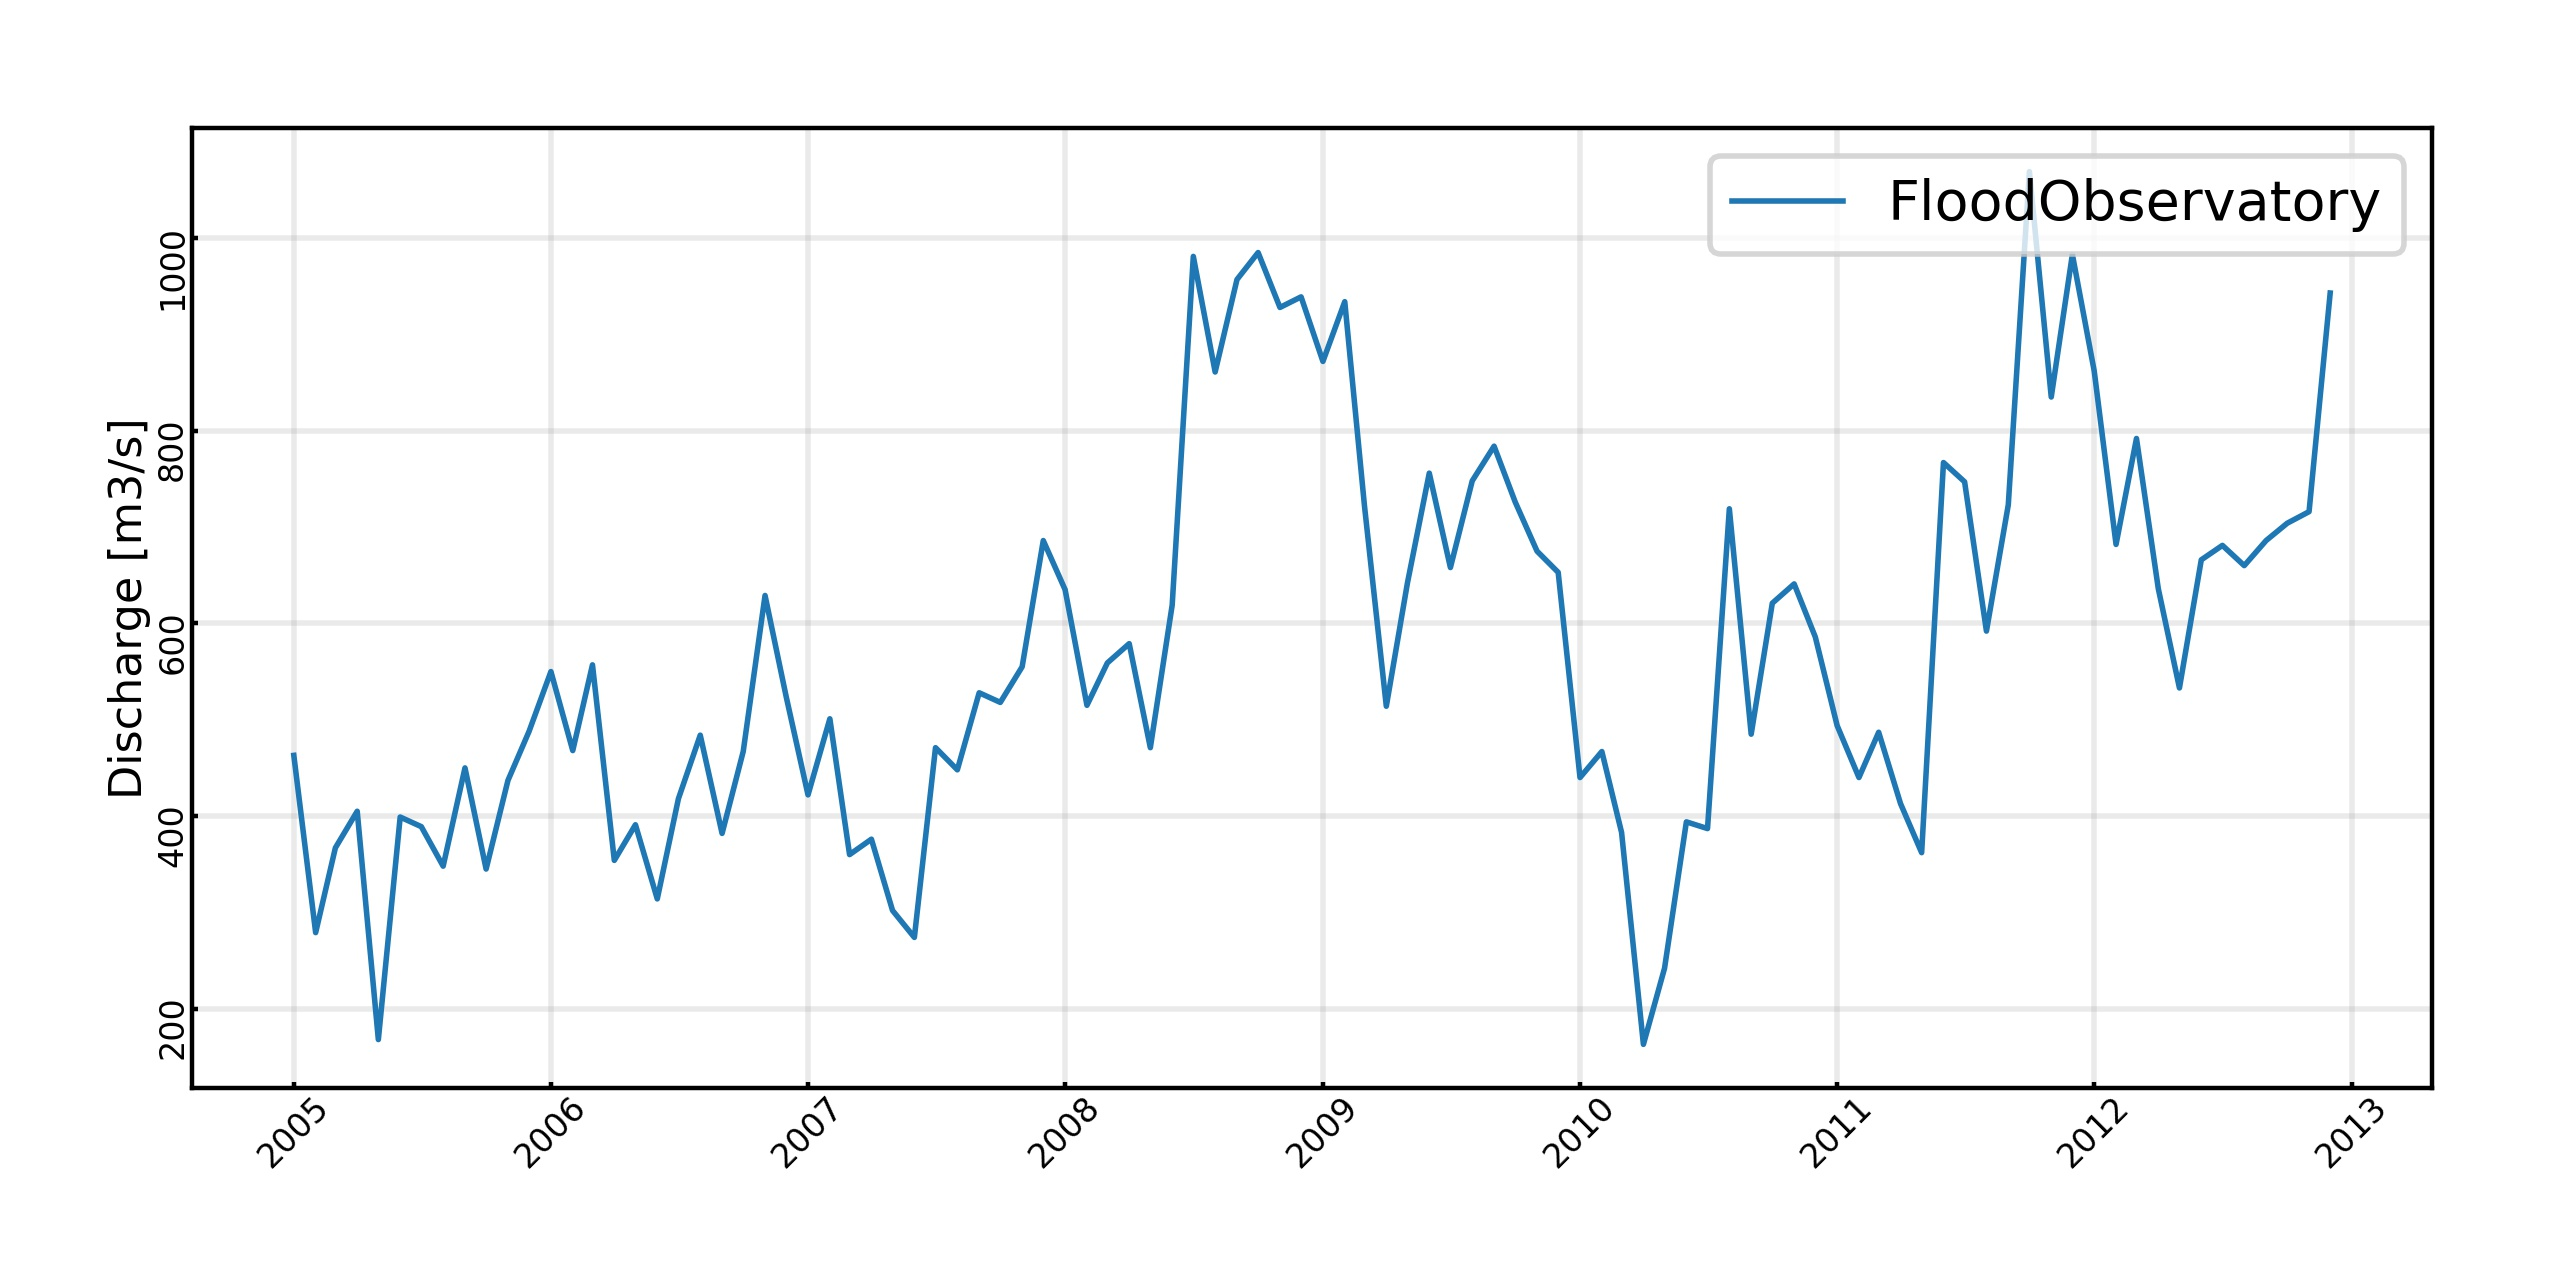
\includegraphics[width=0.8\textwidth]{D:/IHEProjects/TempDev/IHEWAreport/tests/data/area1/fig/fig1e.jpg}%
\caption{Discharge at river mouth of Mindanao River}%
\label{figure:fig2}%
\end{figure}

%
\RaggedRight%
\section{RS data analysis}%
\label{sec:RSdataanalysis}%
The purpose of this study is to select remote sensing products for water accounting, by evaluating the performance of water balance analysis. Three evaluation criteria are applied in the study, Pearson correlation coefficient (PCC), coefficient of determination (R2) and root mean square error (RMSE).%
\linebreak%
PCC - The covariance of the two variables divided by the product of their standard deviations. It has a value between +1 and -1, where 1 is total positive linear correlation, 0 is no linear correlation, and -1 is total negative linear correlation.%
\linebreak%
R2 - The proportion of the variance in the dependent variable that is predictable from the independent variable(s). Best possible score is 1.0 and it can be negative (because the model can be arbitrarily worse).%
\linebreak%
RMSE - The standard deviation of the residuals (prediction errors). It is a measure of how spread out these residuals are. In other words, it tells you how concentrated the data is around the line of best fit.%
\linebreak%
\subsection{Review of RS products}%
\label{subsec:ReviewofRSproducts}%
To evaluate remote sensing products for water balance analysis, three precipitation products, five evapotranspiration products and three GRACE solutions are collected, see Table \ref{table:tab1}. After download products, all data was clipped to Mindanao River Basin. Then the datasets were resampled to spatial resolution of 0.05 degree and aggregated to monthly and yearly time series. The detail description of each product can be found in Annex \ref{annex:products}.%
\linebreak%
\begin{longtable}{|l|l|l|l|l|}%
\caption{Remote sensing products}%
\label{table:tab1}\\%
\hline%
\textbf{Product}&\textbf{Type}&\textbf{Duration}&\textbf{Temporal Res.}&\textbf{Spatial Res.}\\%
\hline%
\endfirsthead%
\hline%
Product&Type&Duration&Temporal Res.&Spatial Res.\\%
\hline%
\endhead%
\hline%
\endfoot%
ALEXI&Evapotranspiration&2005 - 2012&daily&$0.05^{o}$\\%
CMRSET&Evapotranspiration&2005 - 2012&monthly&$0.05^{o}$\\%
GLEAM&Evapotranspiration&2005 - 2012&monthly&$0.25^{o}$\\%
MOD16A2&Evapotranspiration&2005 - 2012&eight-daily&463m\\%
SSEBop&Evapotranspiration&2005 - 2012&monthly&1km\\%
CHIRPS&Precipitation&2005 - 2012&monthly&$0.05^{o}$\\%
GPM&Precipitation&2005 - 2012&monthly&$0.1^{o}$\\%
TRMM&Precipitation&2005 - 2012&monthly&$0.25^{o}$\\%
CSR&GRACE&2005 - 2012&quasi-monthly&$1^{o}$\\%
GFZ&GRACE&2005 - 2012&quasi-monthly&$1^{o}$\\%
JPL&GRACE&2005 - 2012&quasi-monthly&$1^{o}$\\%
\end{longtable}%
\subsubsection{Precipitation products}%
\label{ssubsec:Precipitationproducts}%
The precipitation products present similar pattern. Figure \ref{figure:fig3} shows the time series plots of precipitation from the three products. There is no missing values from 2005 to 2013. CHIRPS has the higher precipitation in the summer.%
\linebreak%


\begin{figure}[H]%
\centering%
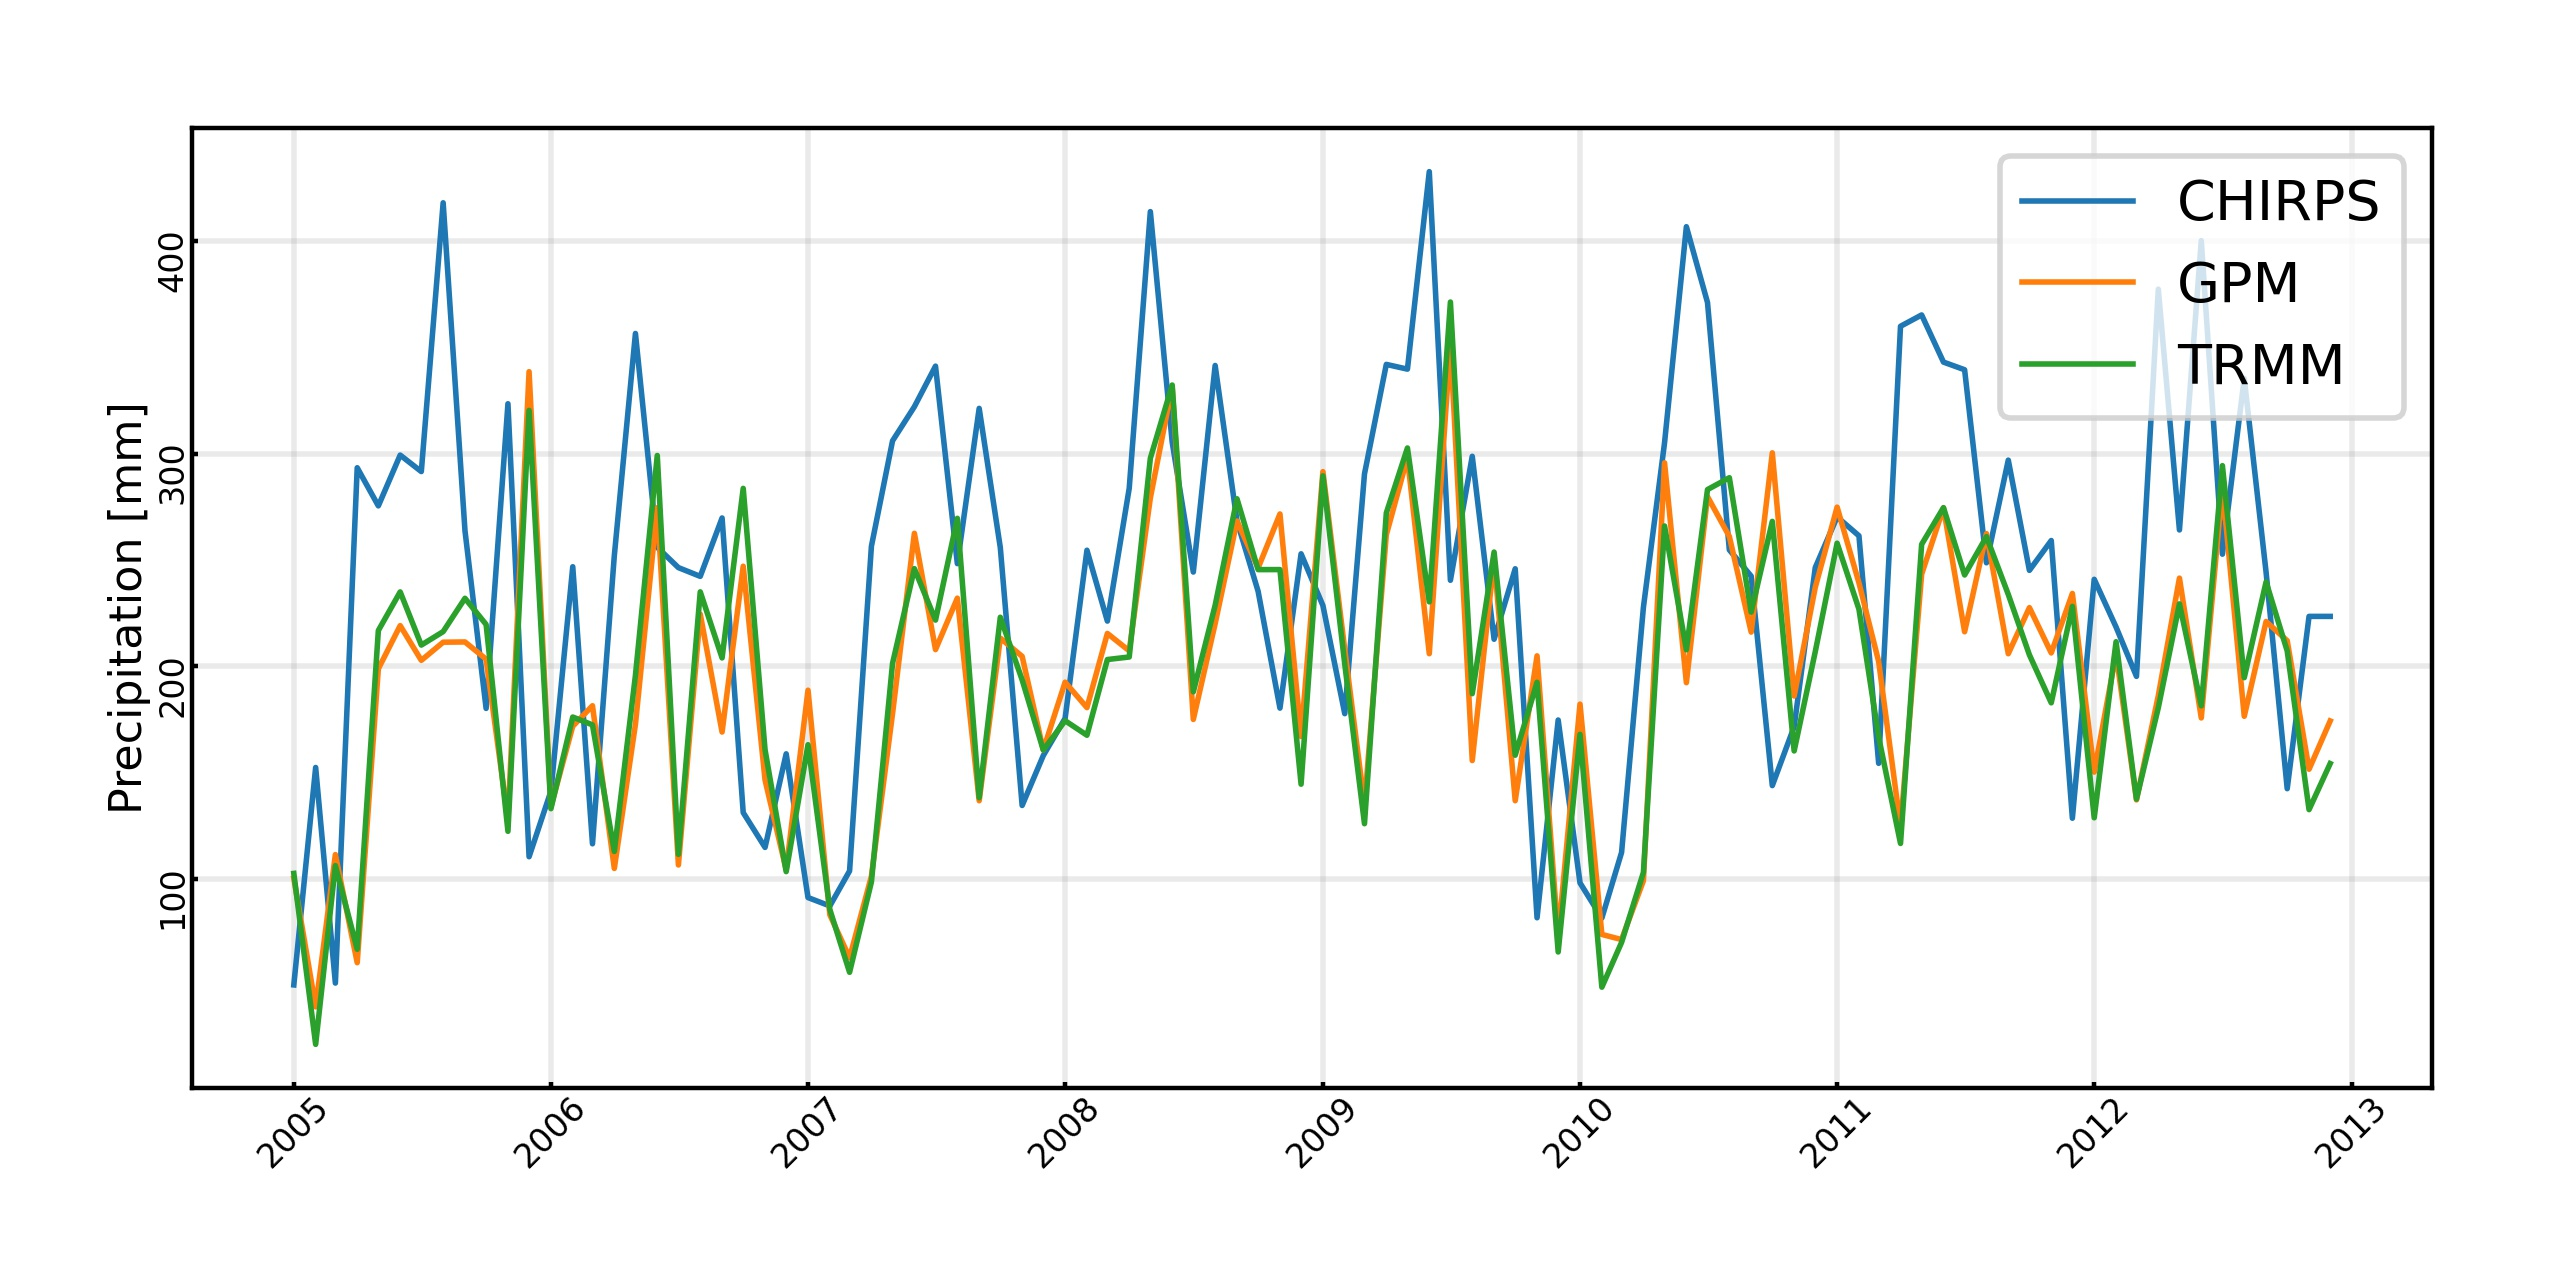
\includegraphics[width=0.8\textwidth]{D:/IHEProjects/TempDev/IHEWAreport/tests/data/area1/fig/fig1a.jpg}%
\caption{Precipitation products for Mindanao River Basin}%
\label{figure:fig3}%
\end{figure}

%
Figure \ref{figure:fig4} shows the correlation between the products. TRMM and GPM obtained the highest correlation with PCC of 0.97, while CHIRPS versus GPM had the lowest PCC of 0.29.%
\linebreak%


\begin{figure}[H]%
\centering%
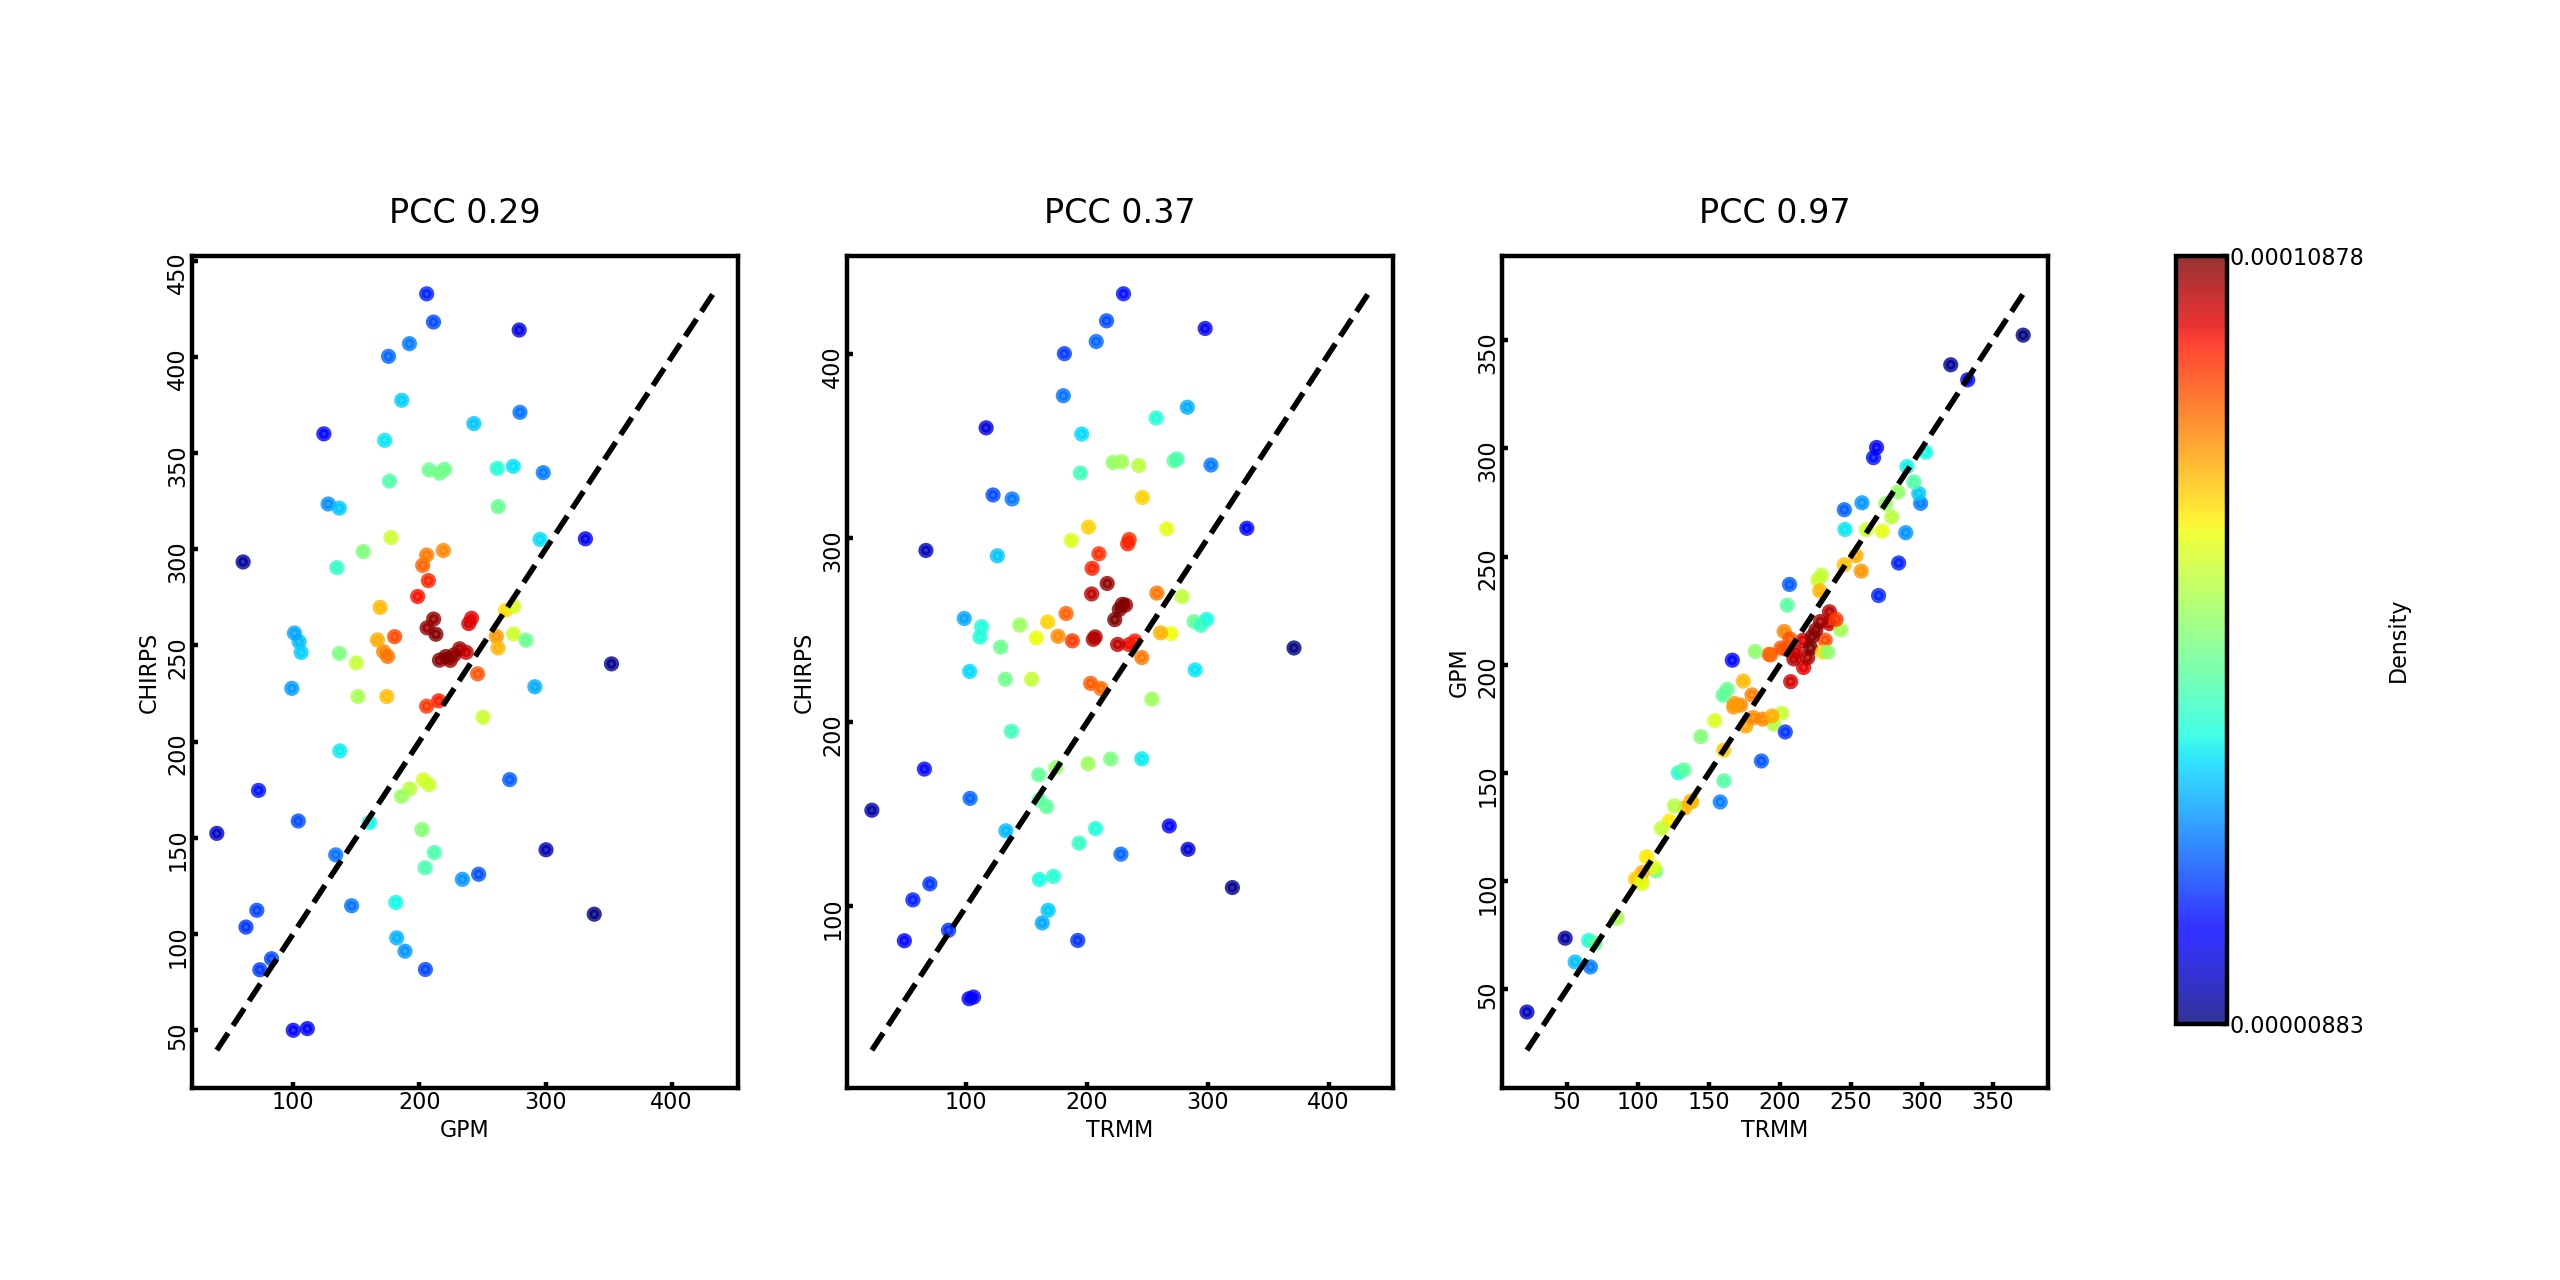
\includegraphics[width=0.8\textwidth]{D:/IHEProjects/TempDev/IHEWAreport/tests/data/area1/fig/fig2a.jpg}%
\caption{Correlation between precipitation products (unit: mm/month)}%
\label{figure:fig4}%
\end{figure}

%
The monthly mean and annual precipitation from the products are illustrated in the Figure \ref{figure:fig5} and Figure \ref{figure:fig6}. CHIRPS had highest values in wet season while TRMM shows lowest values in dry months. GPM values were largely between CHIRPS and TRMM in most of the months. The annual precipitation values do not show significant differences either among the different products except for 2012 when CHIRPS showed a significant higher value compared to the other products (up to 85 mm/year)%
\linebreak%


\begin{figure}[H]%
\centering%
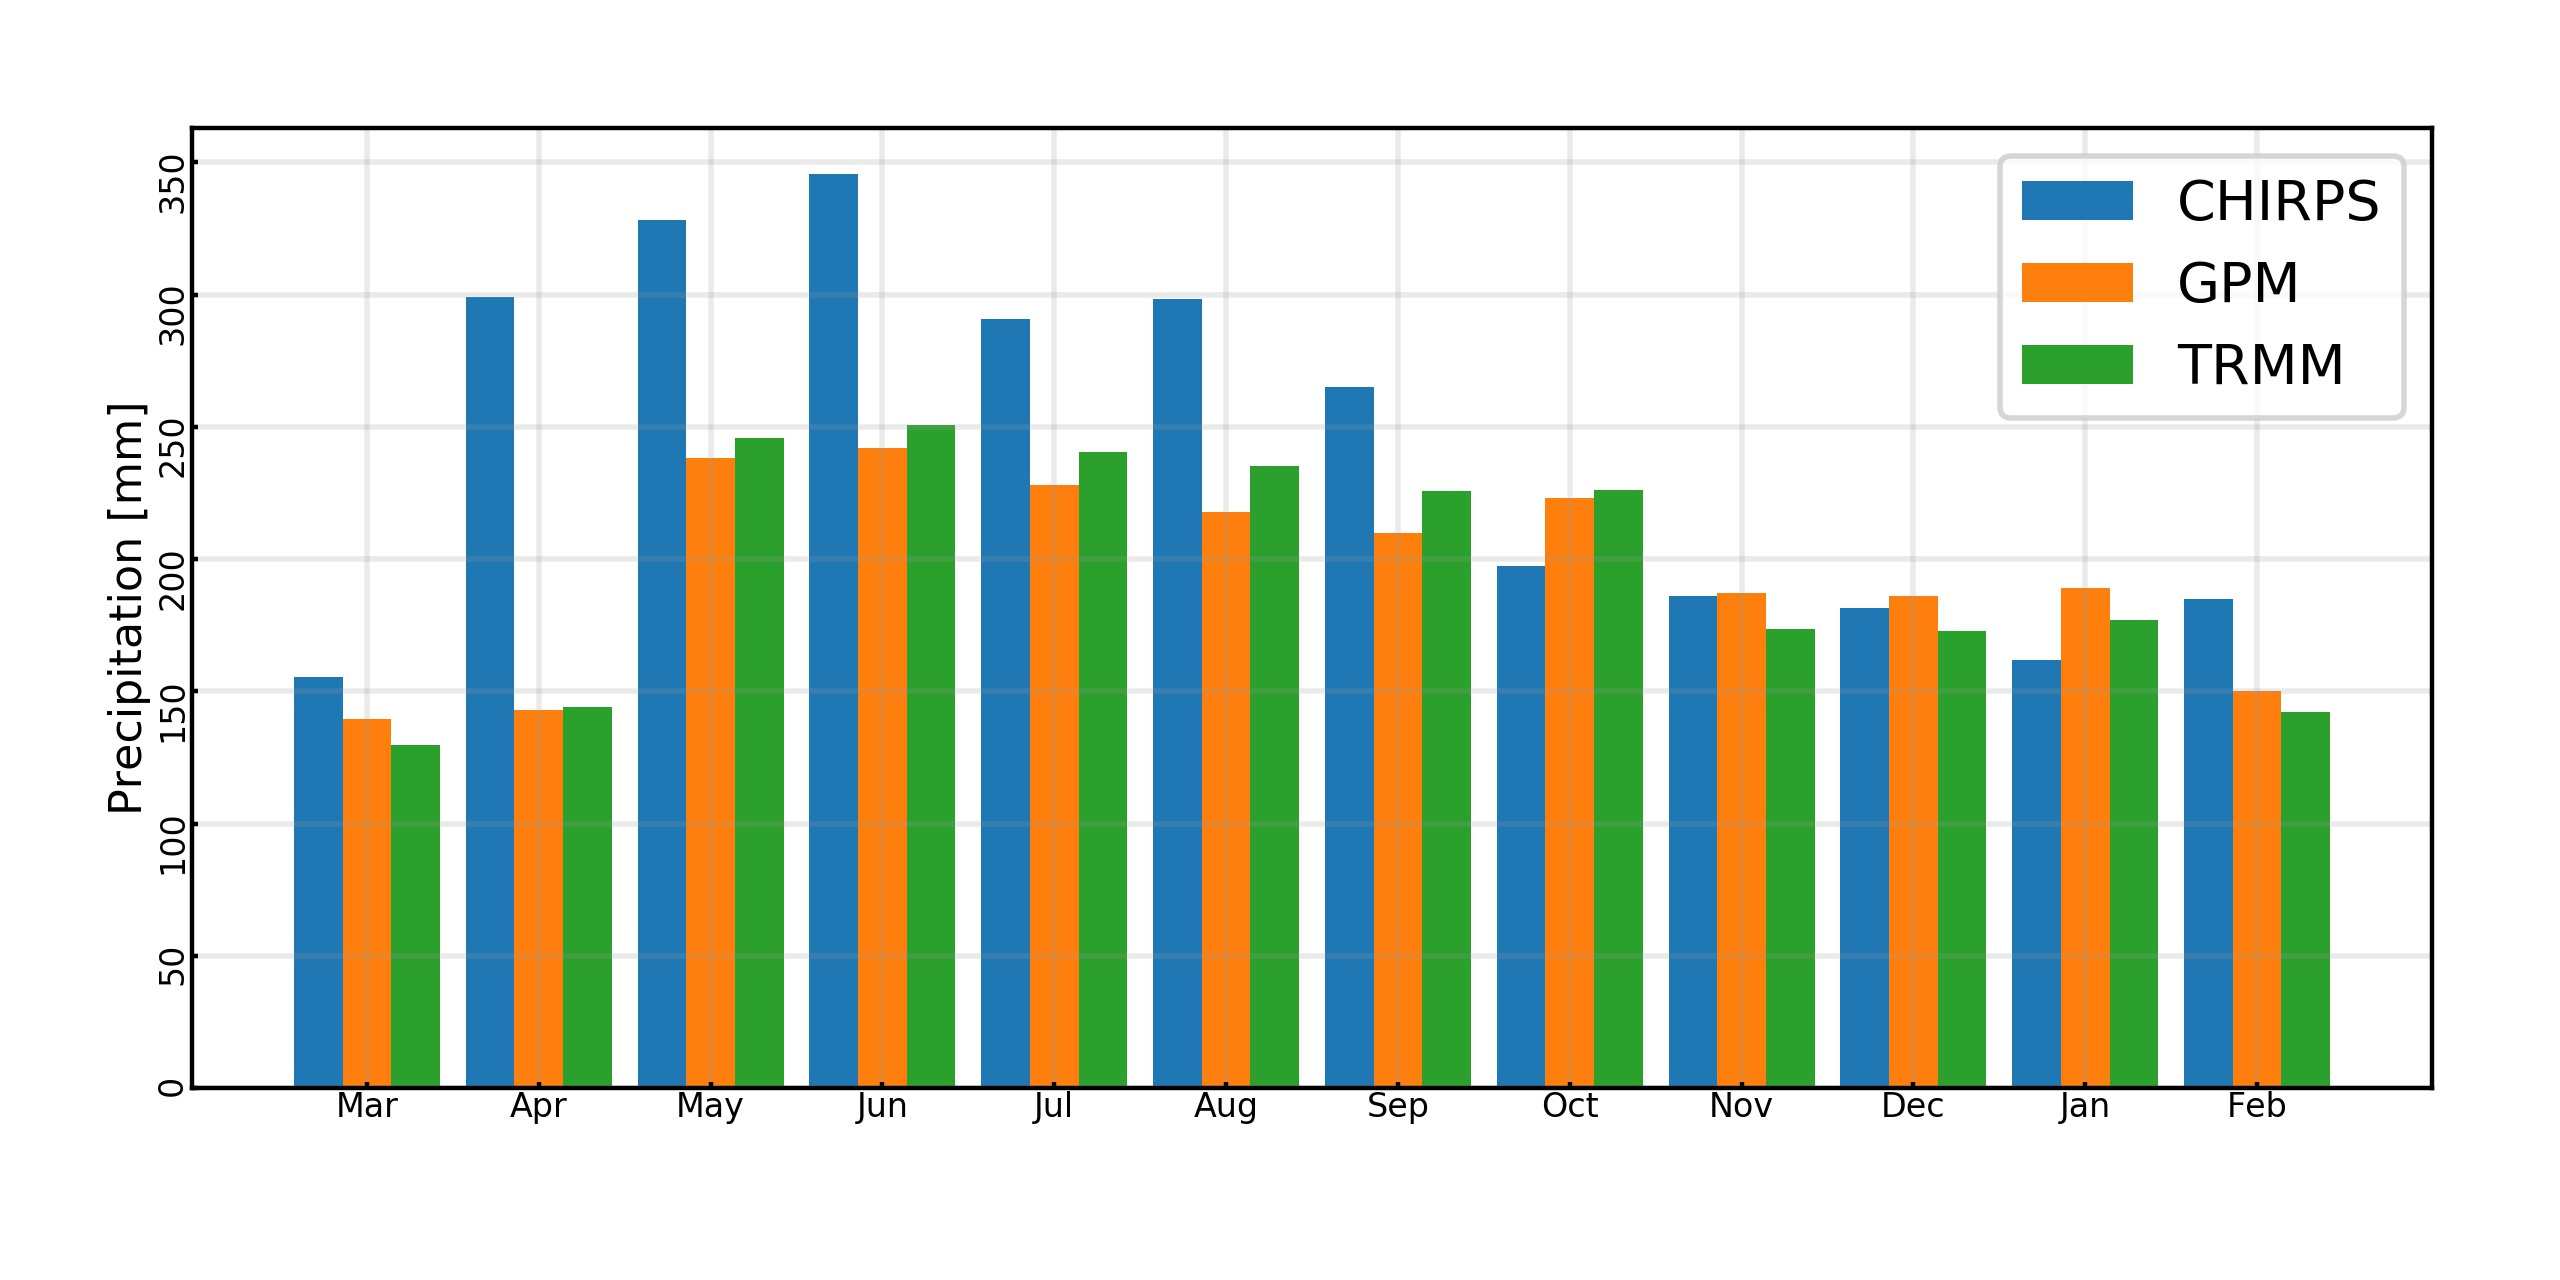
\includegraphics[width=0.8\textwidth]{D:/IHEProjects/TempDev/IHEWAreport/tests/data/area1/fig/fig3a_monthly.jpg}%
\caption{Monthly mean precipitation for Mindanao River Basin}%
\label{figure:fig5}%
\end{figure}

%


\begin{figure}[H]%
\centering%
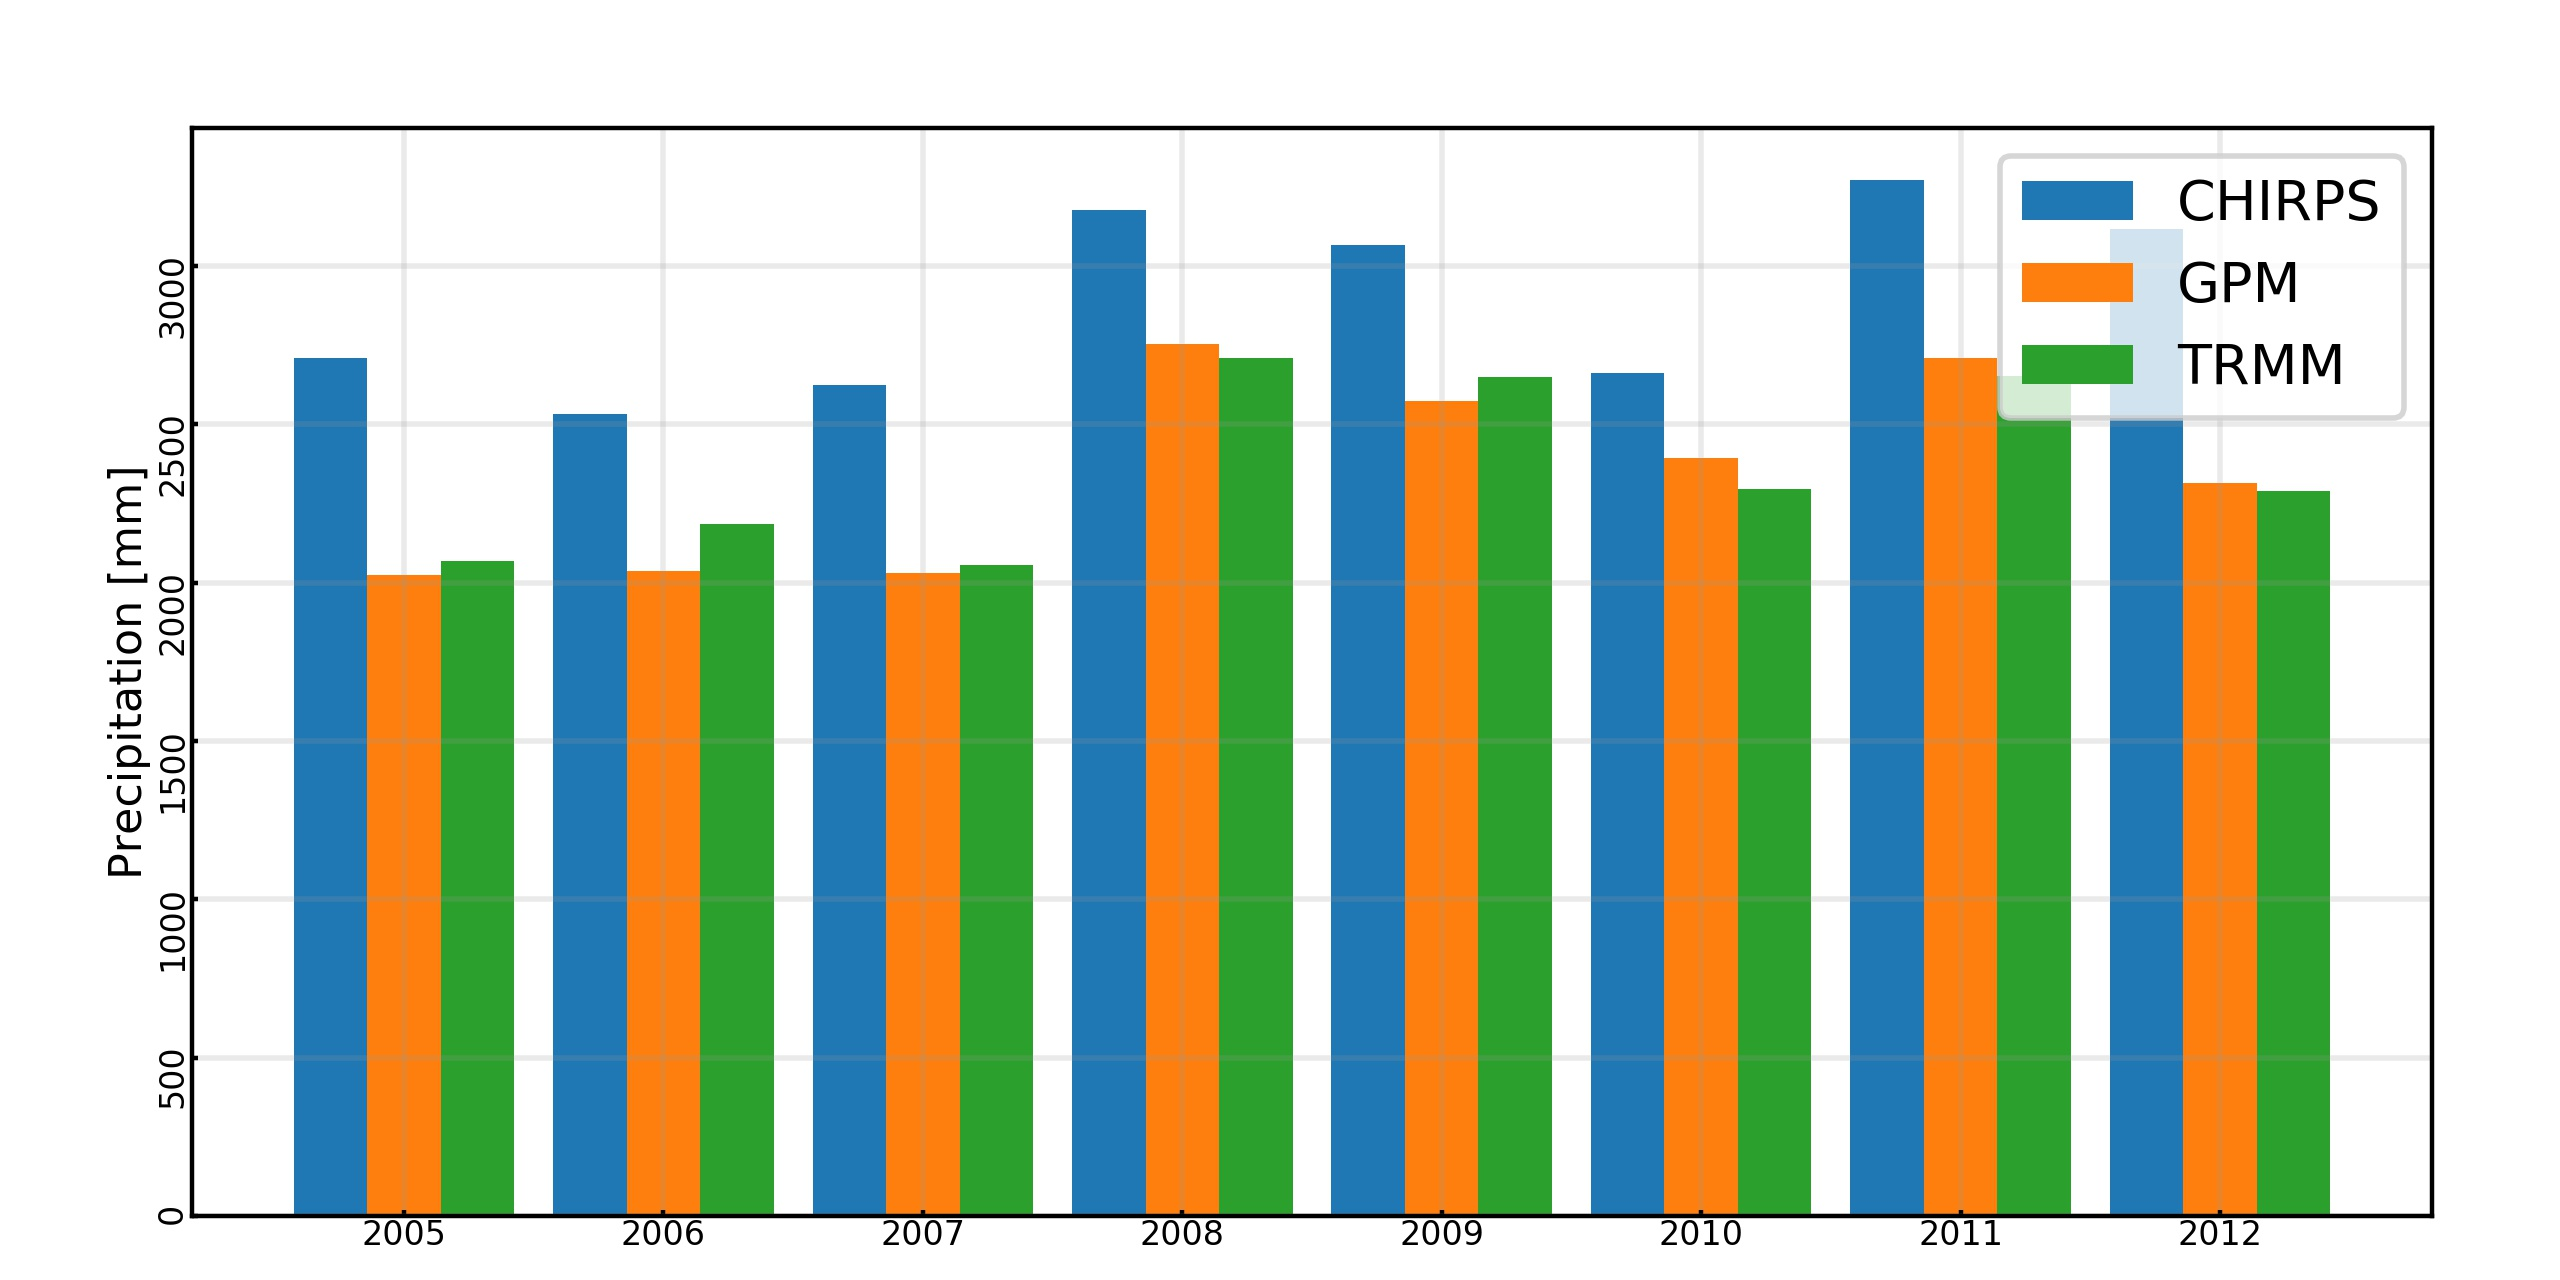
\includegraphics[width=0.8\textwidth]{D:/IHEProjects/TempDev/IHEWAreport/tests/data/area1/fig/fig3a_yearly.jpg}%
\caption{Annual precipitation for Mindanao River Basin}%
\label{figure:fig6}%
\end{figure}

%
\subsubsection{Evapotranspiration products}%
\label{ssubsec:Evapotranspirationproducts}%
The evapotranspiration products have similar pattern. Figure \ref{figure:fig7} shows the time series plots of precipitation from the five products. CHIRPS has the higher precipitation in the summer.%
\linebreak%


\begin{figure}[H]%
\centering%
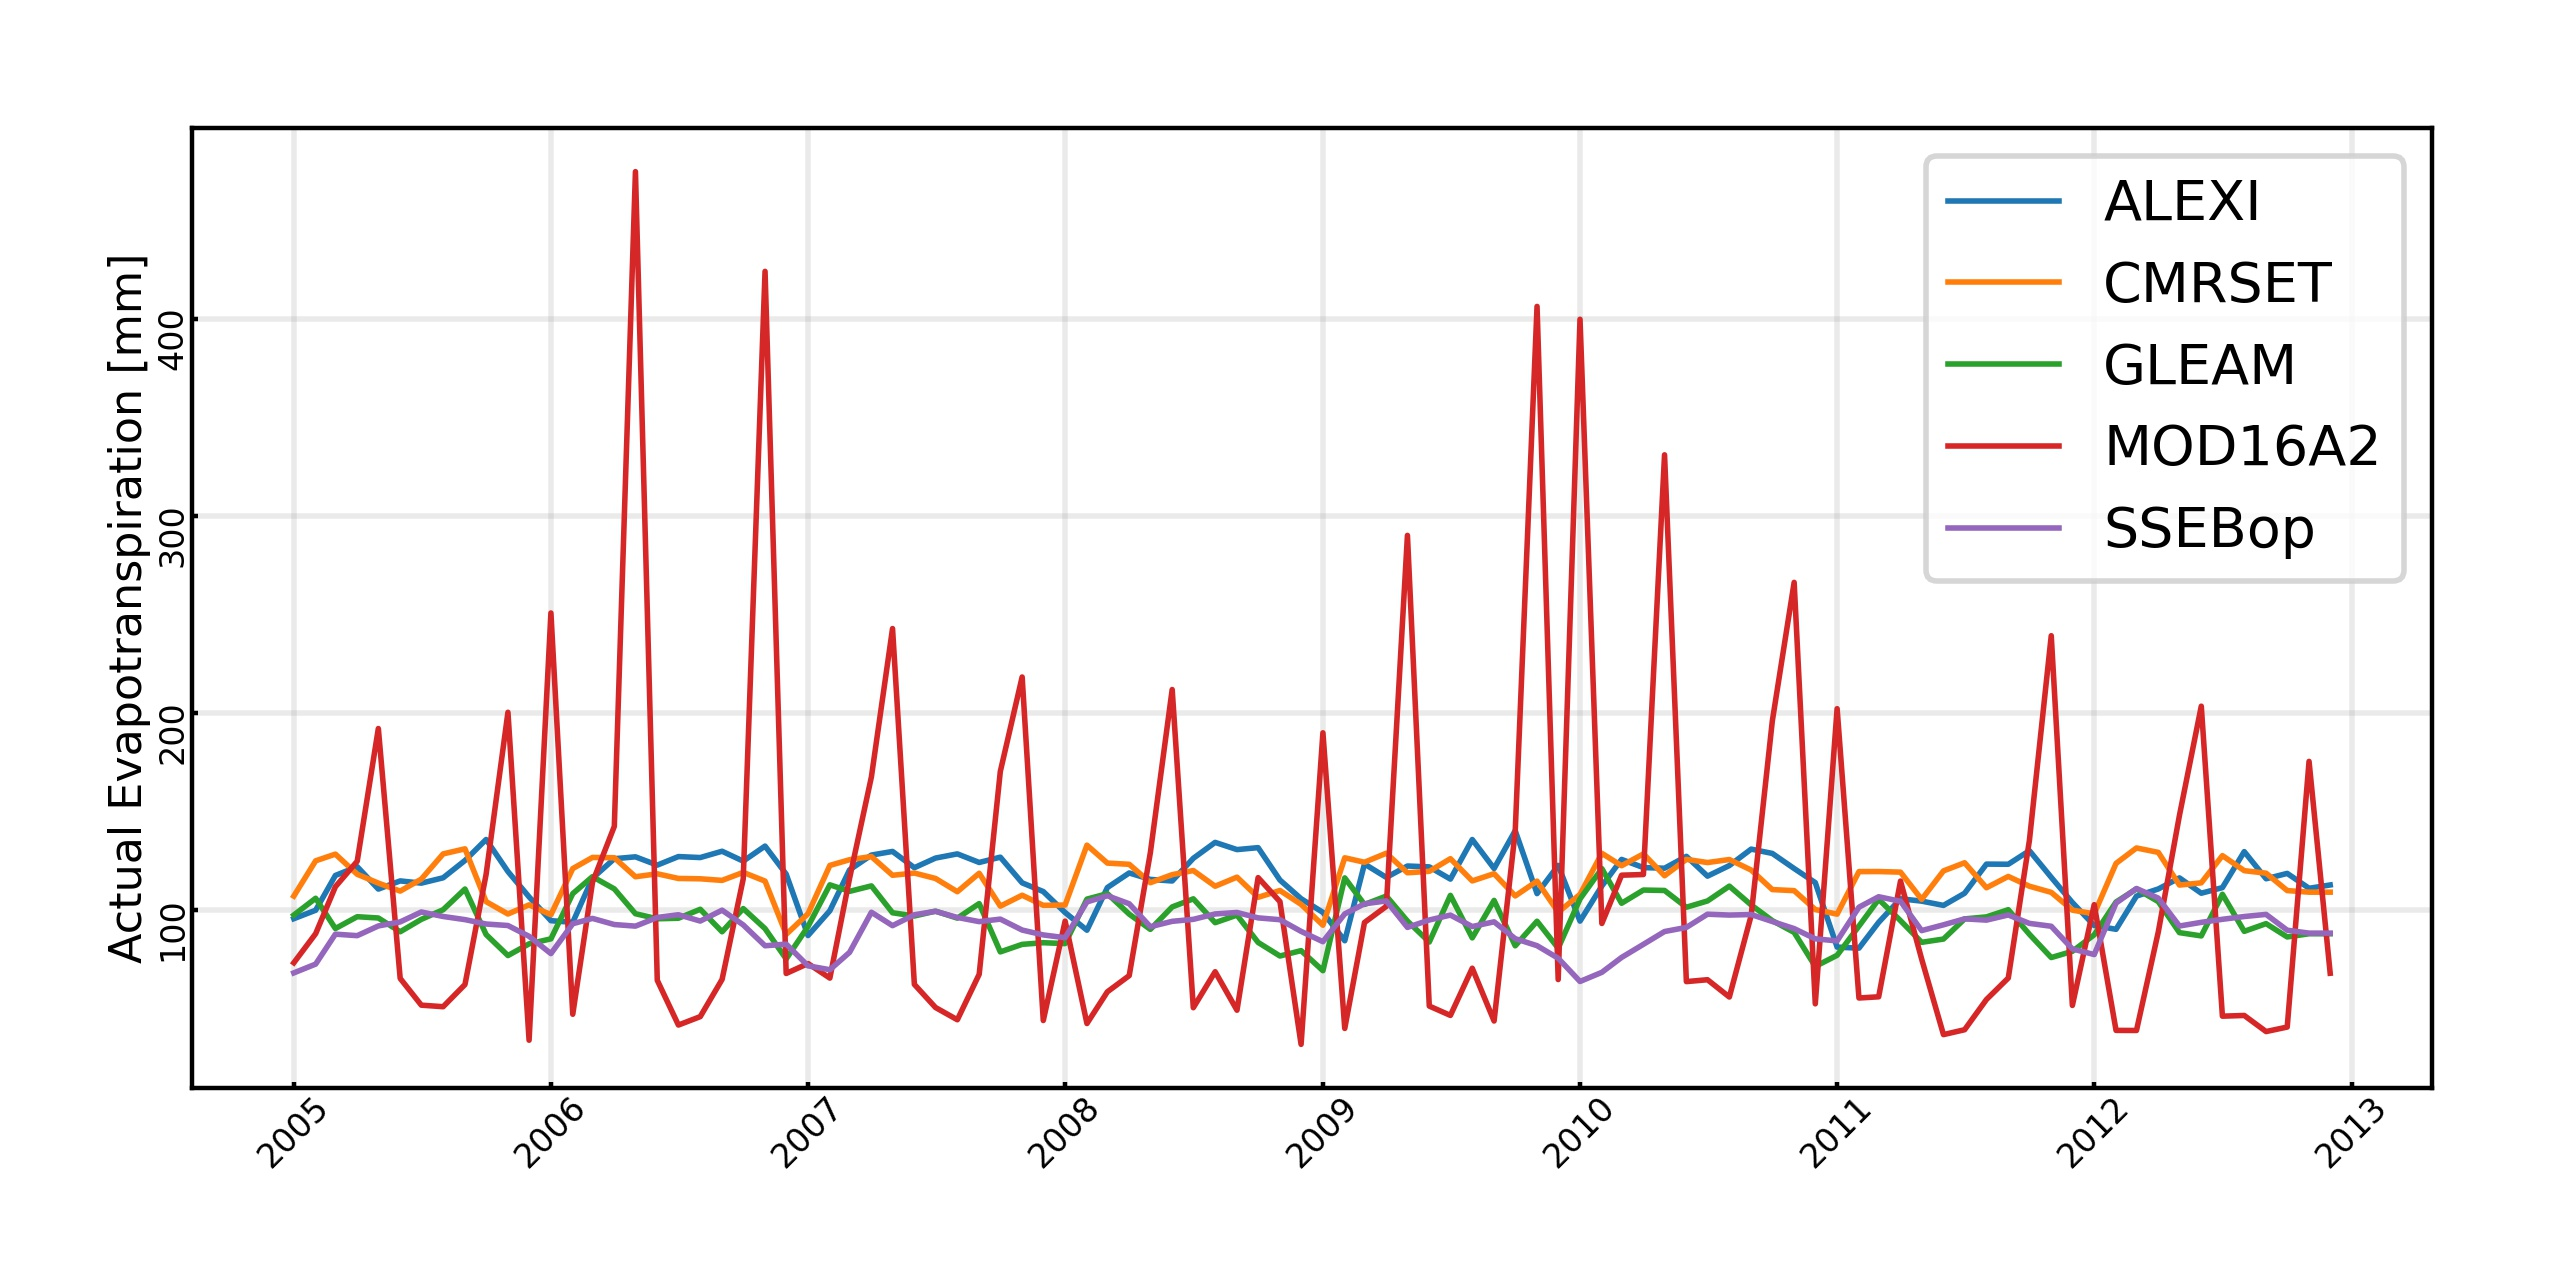
\includegraphics[width=0.8\textwidth]{D:/IHEProjects/TempDev/IHEWAreport/tests/data/area1/fig/fig1b.jpg}%
\caption{Annual evapotranspiration  for Mindanao River Basin}%
\label{figure:fig7}%
\end{figure}

%
In terms of correlation, CMRSET and GLEAM showed the highest correlation with PCC of 0.82, while  SSEBop versus  MOD16A2 had the lowest PCC of  -0.3, see Figure \ref{figure:fig8}.%
\linebreak%


\begin{figure}[H]%
\centering%
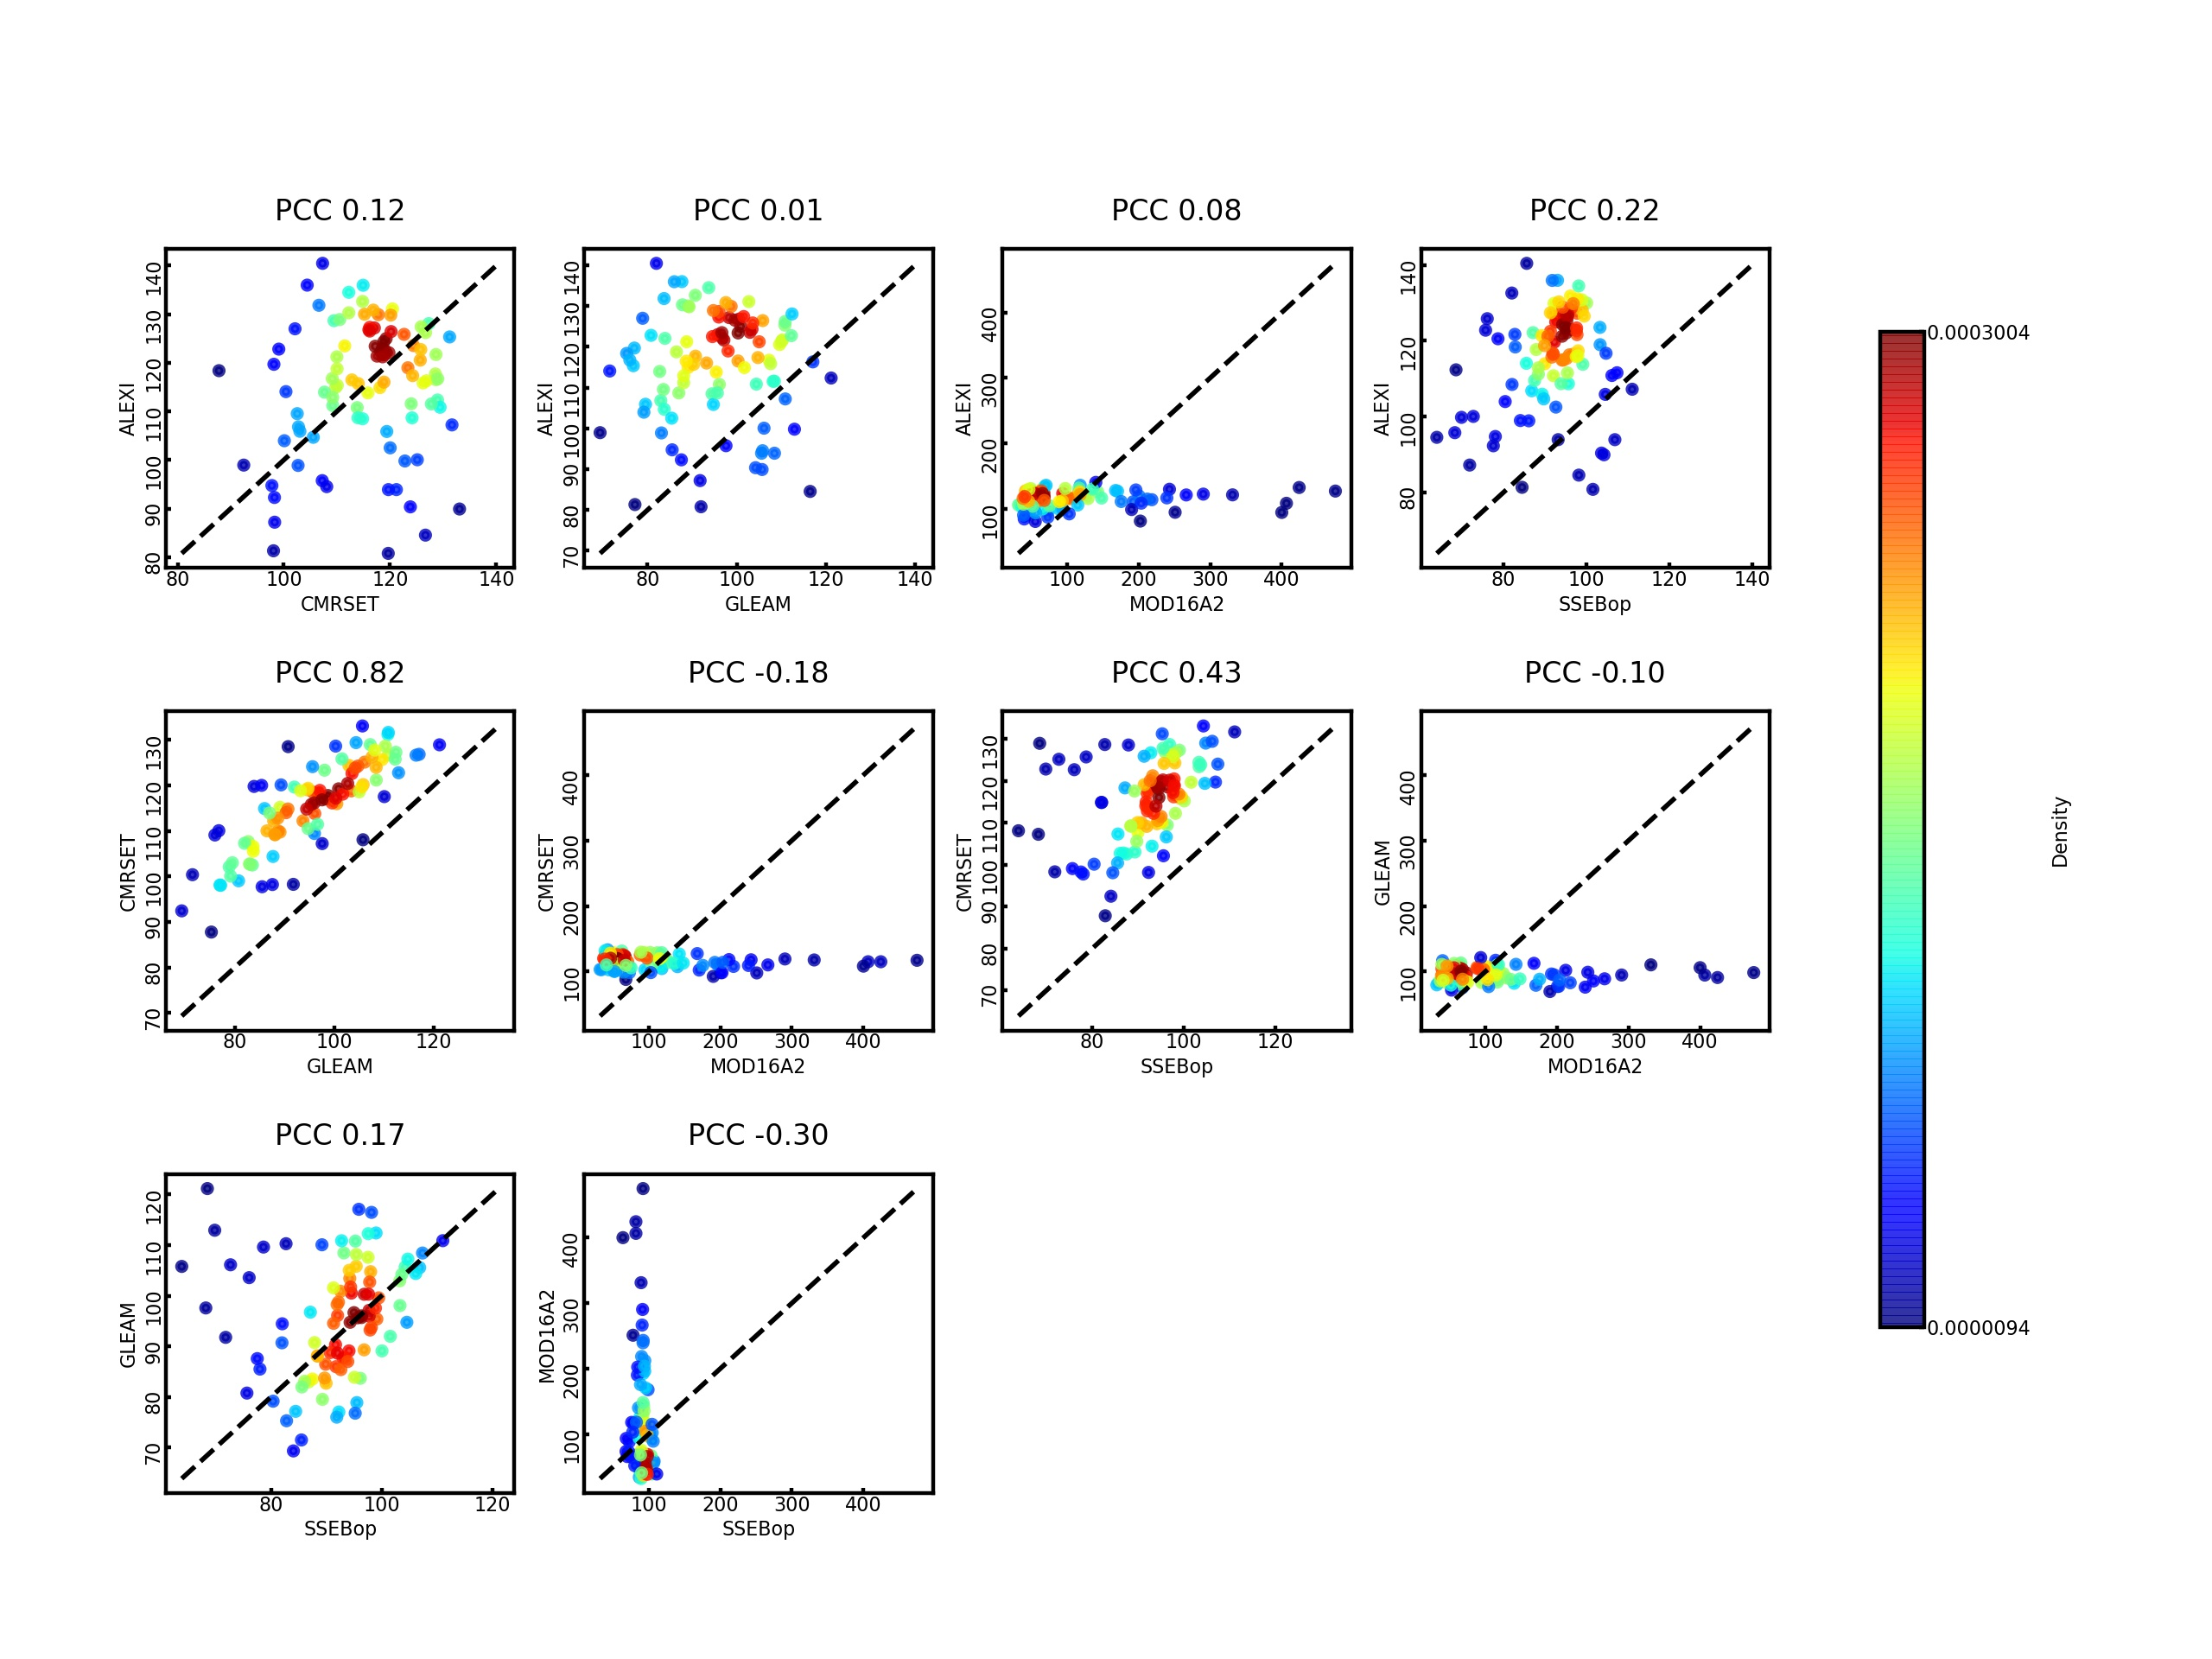
\includegraphics[width=0.8\textwidth]{D:/IHEProjects/TempDev/IHEWAreport/tests/data/area1/fig/fig2b.jpg}%
\caption{Correlation between actual evapotranspiration products (unit: mm/month)}%
\label{figure:fig8}%
\end{figure}

%
The monthly mean and annual actual evapotranspiration from the products are plotted in the Figure \ref{figure:fig9} and Figure \ref{figure:fig10}. The highest values in wet season was occurred in MOD16A2 while MOD16A2 presented highest values in dry months. GLEAM values were largely between MOD16A2 and CMRSET in most of the months.%
\linebreak%
The annual actual evapotranspiration values do not show significant differences either among the different products except for 2010 when MOD16A2 showed a significant higher value compared to the other products (up to 800mm/year)%
\linebreak%


\begin{figure}[H]%
\centering%
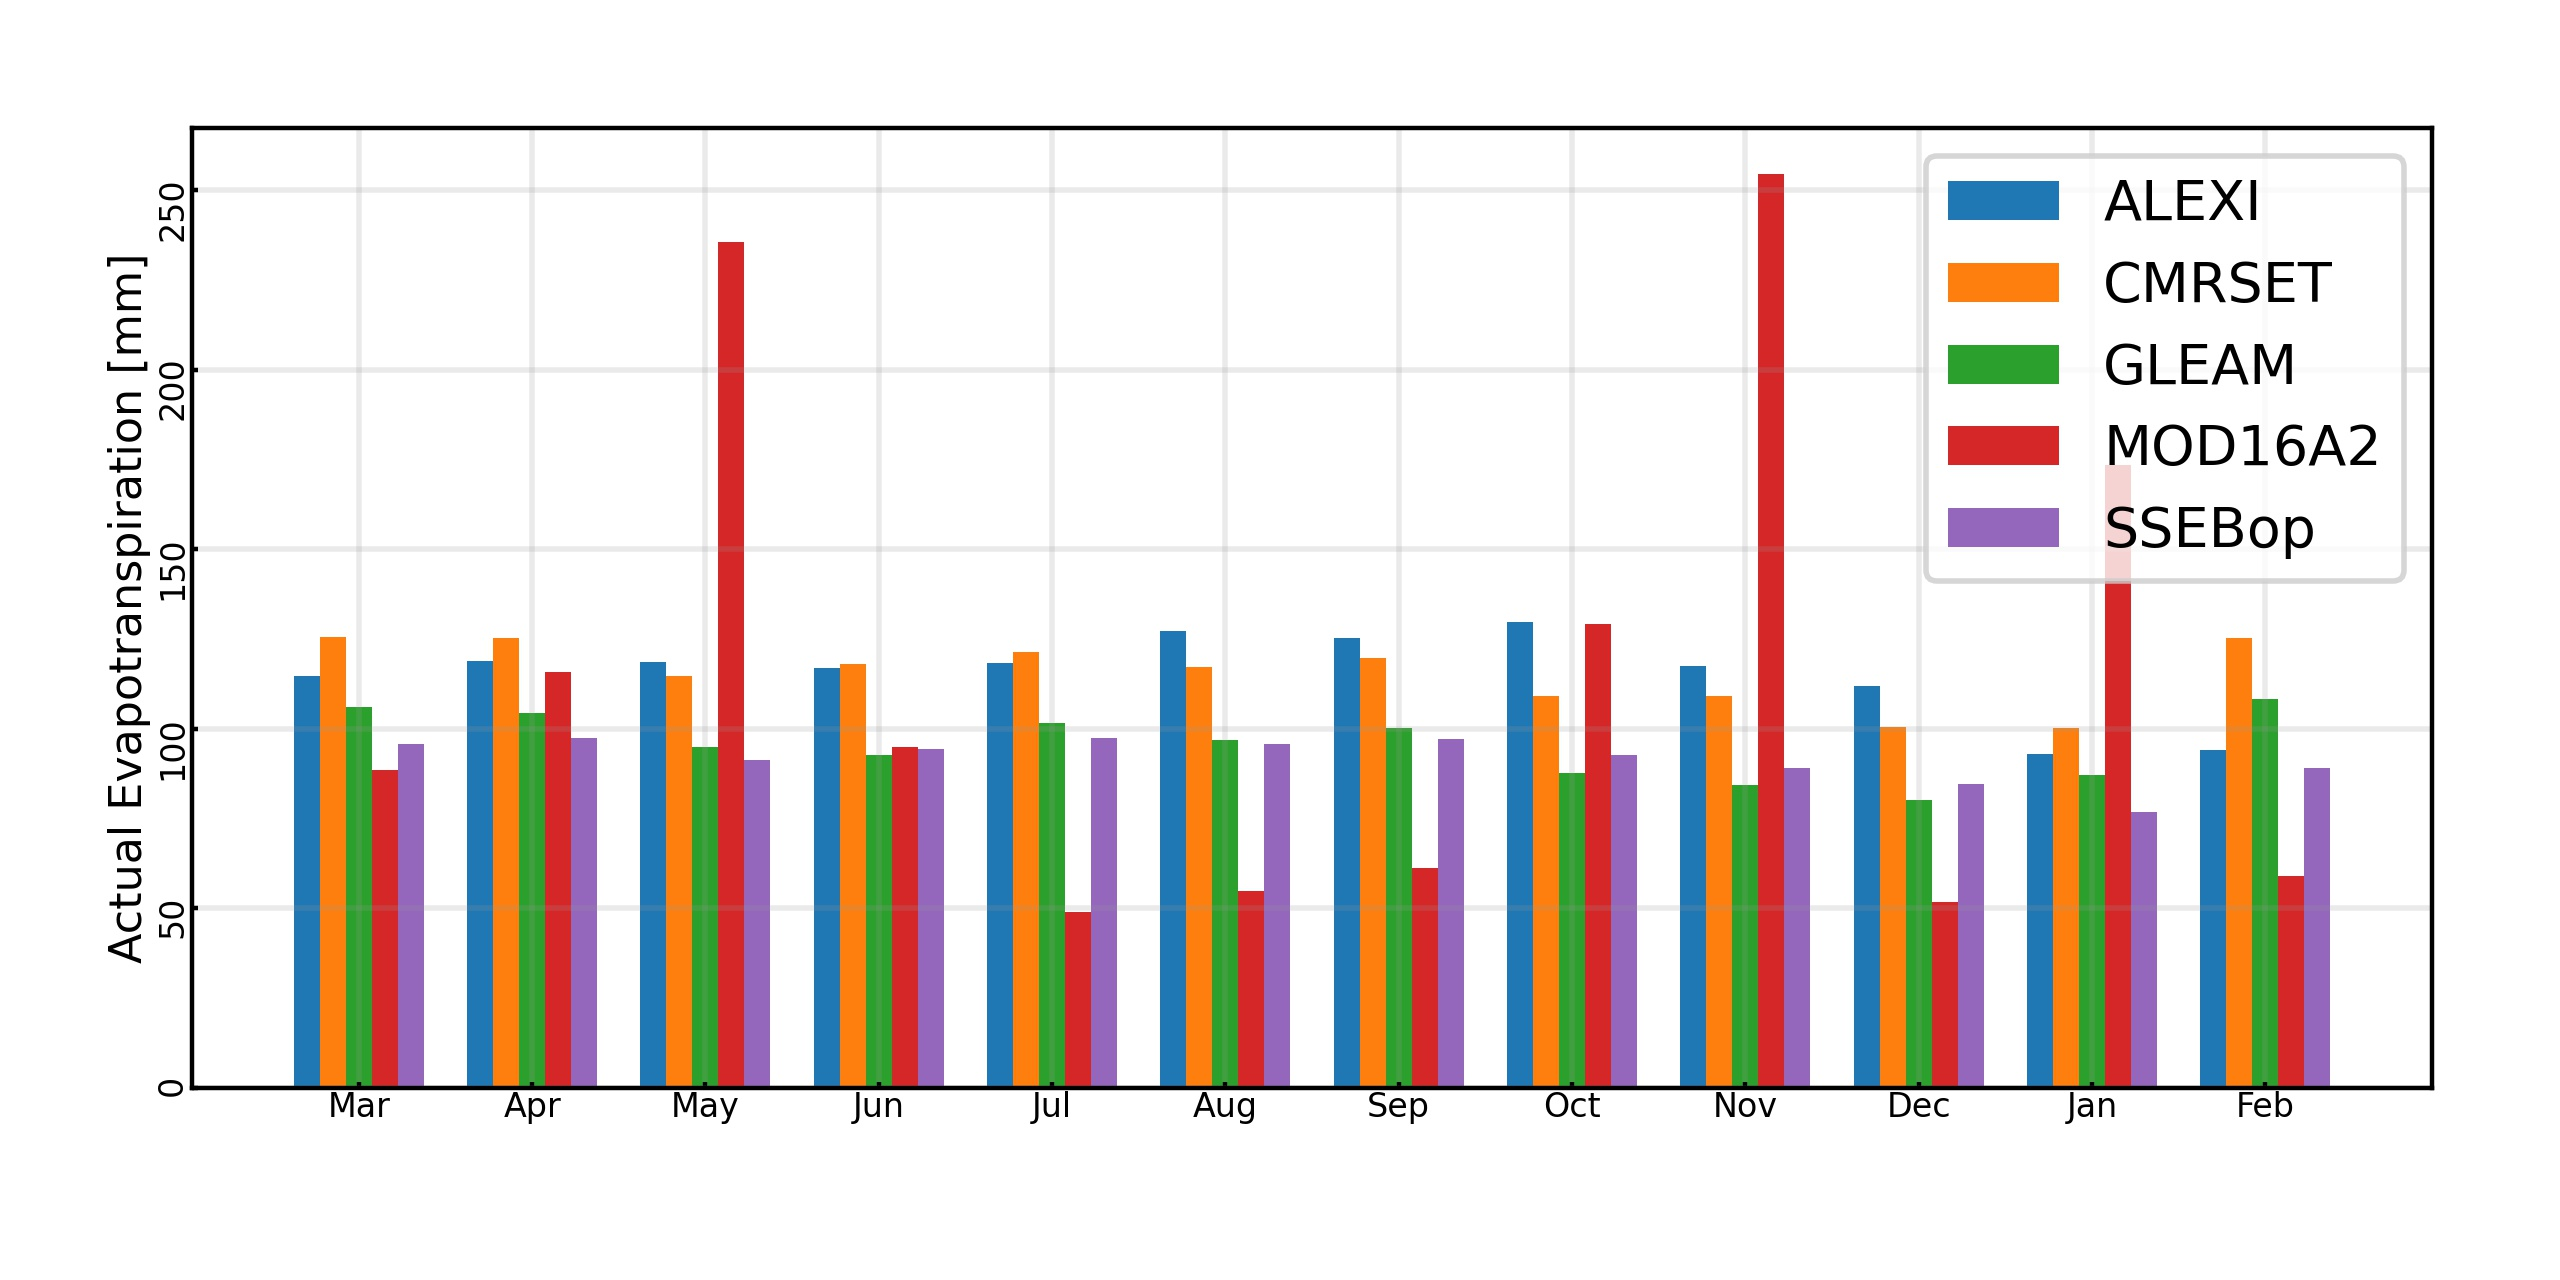
\includegraphics[width=0.8\textwidth]{D:/IHEProjects/TempDev/IHEWAreport/tests/data/area1/fig/fig3b_monthly.jpg}%
\caption{Monthly mean actual evapotranspiration for Mindanao River Basin}%
\label{figure:fig9}%
\end{figure}

%


\begin{figure}[H]%
\centering%
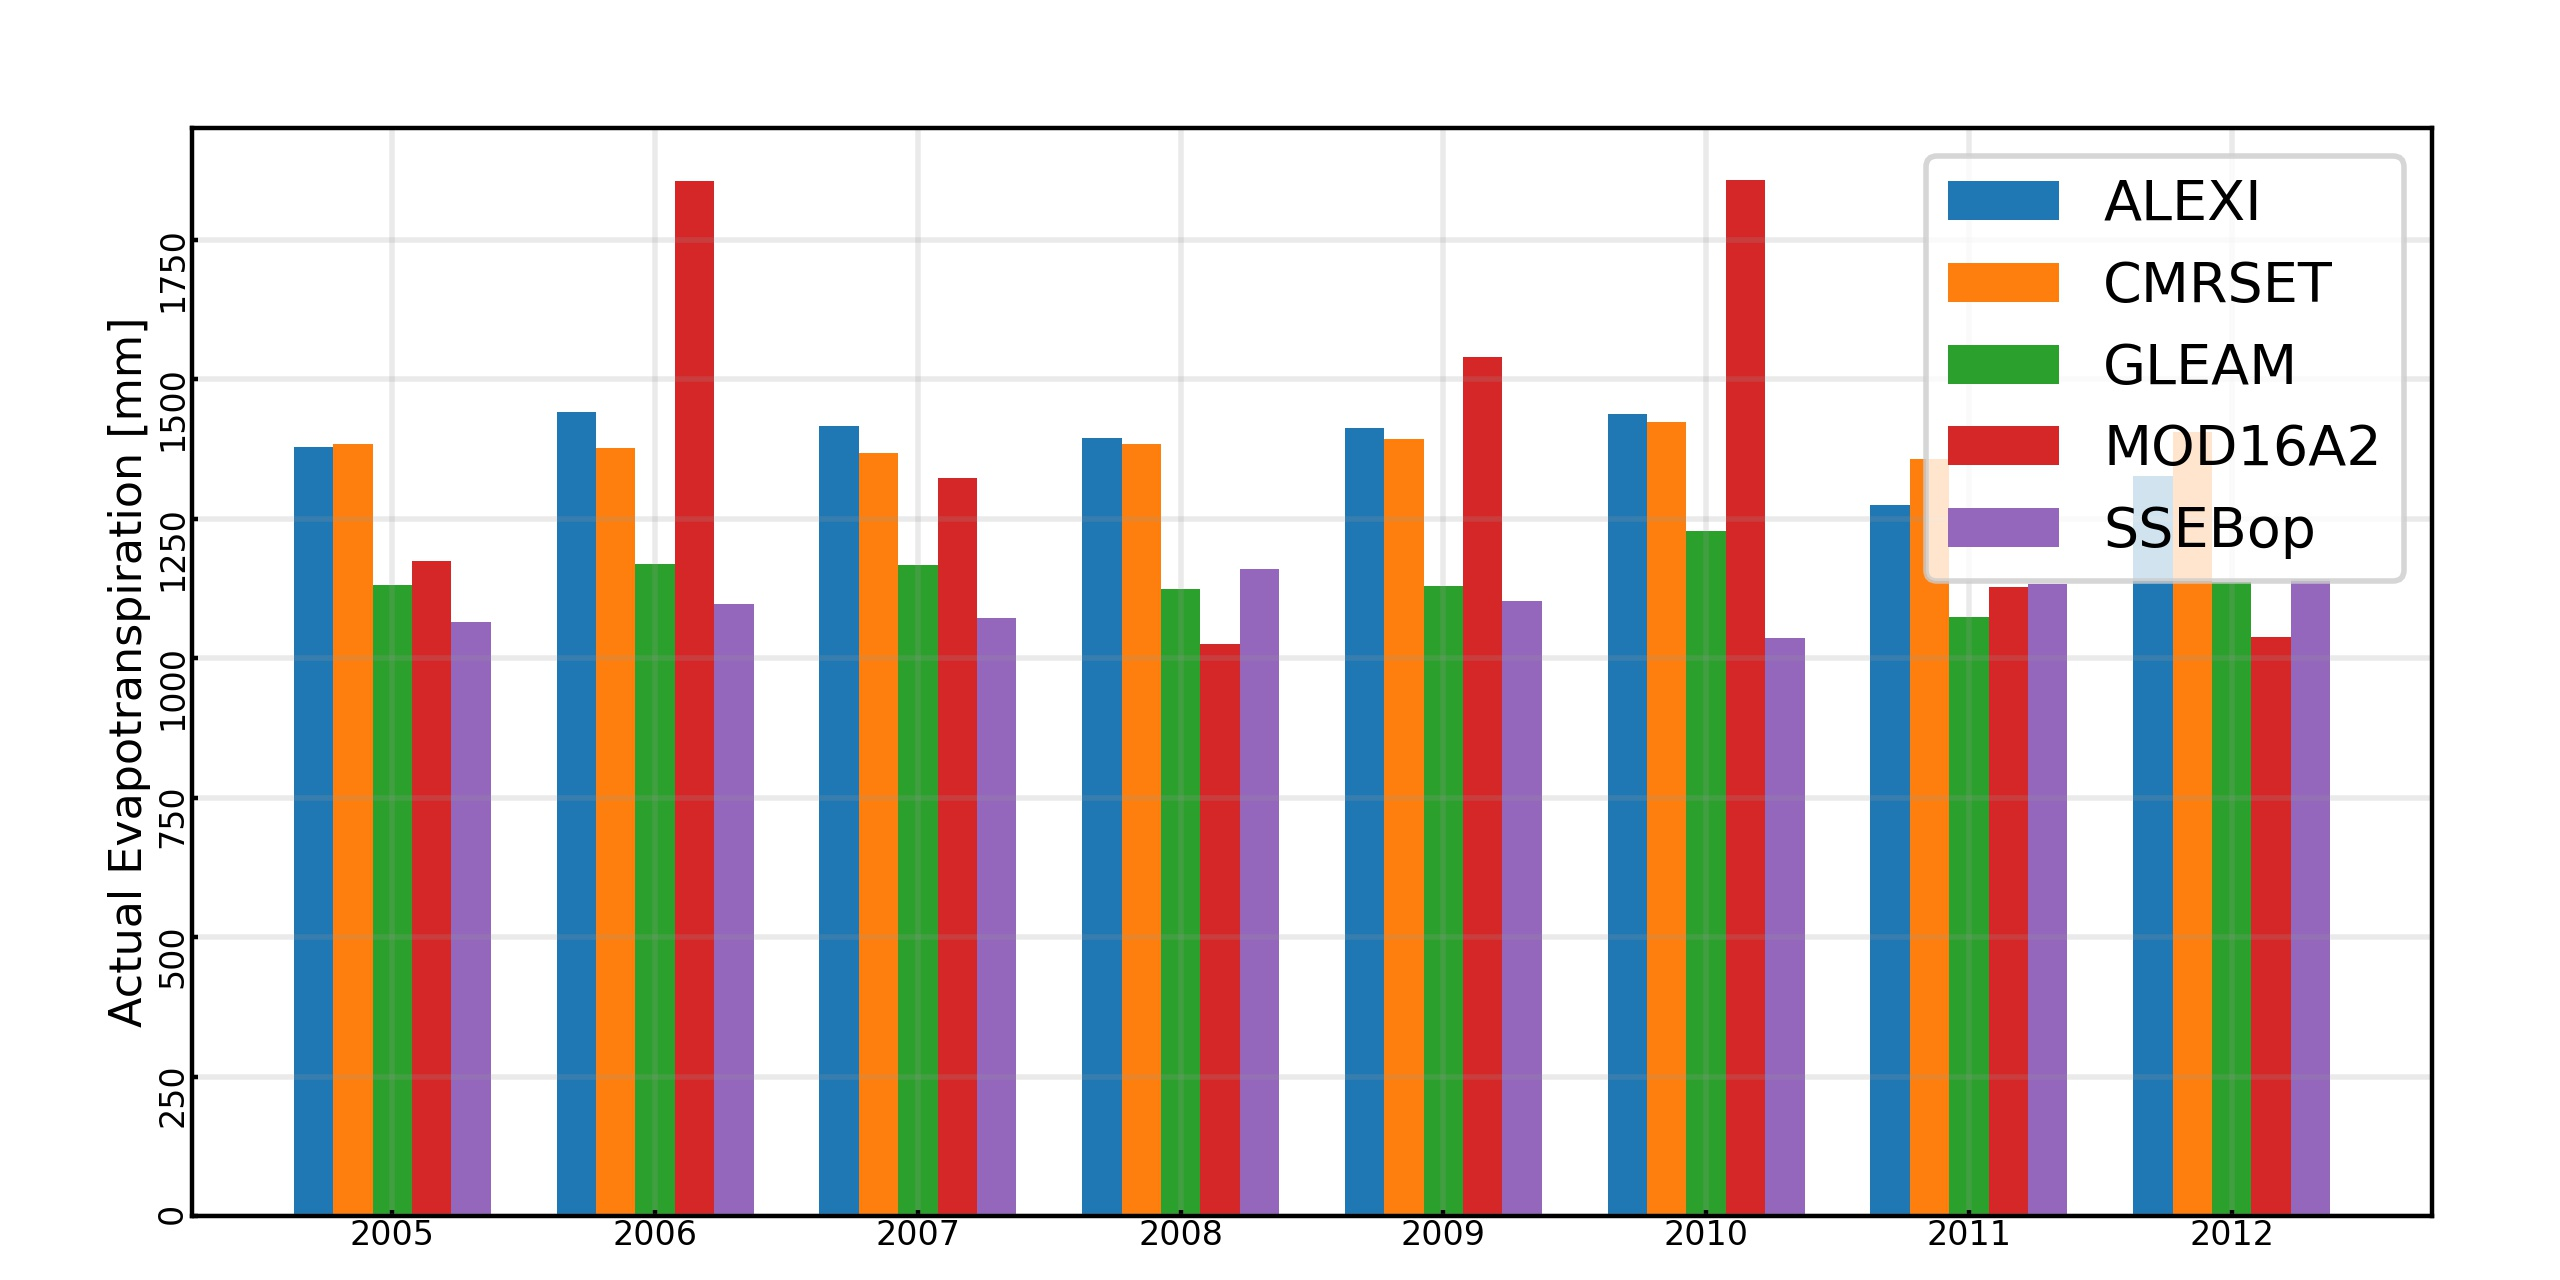
\includegraphics[width=0.8\textwidth]{D:/IHEProjects/TempDev/IHEWAreport/tests/data/area1/fig/fig3b_yearly.jpg}%
\caption{Annual actual evapotranspiration for Mindanao River Basin}%
\label{figure:fig10}%
\end{figure}

%
\subsubsection{Grace solutions (change in storage)}%
\label{ssubsec:Gracesolutions(changeinstorage)}%
The GRACE products show similar pattern. Figure \ref{figure:fig11} is the time series plots of precipitation from the three products. CSR estimates larger dynamic of storage change compare with other products.%
\linebreak%


\begin{figure}[H]%
\centering%
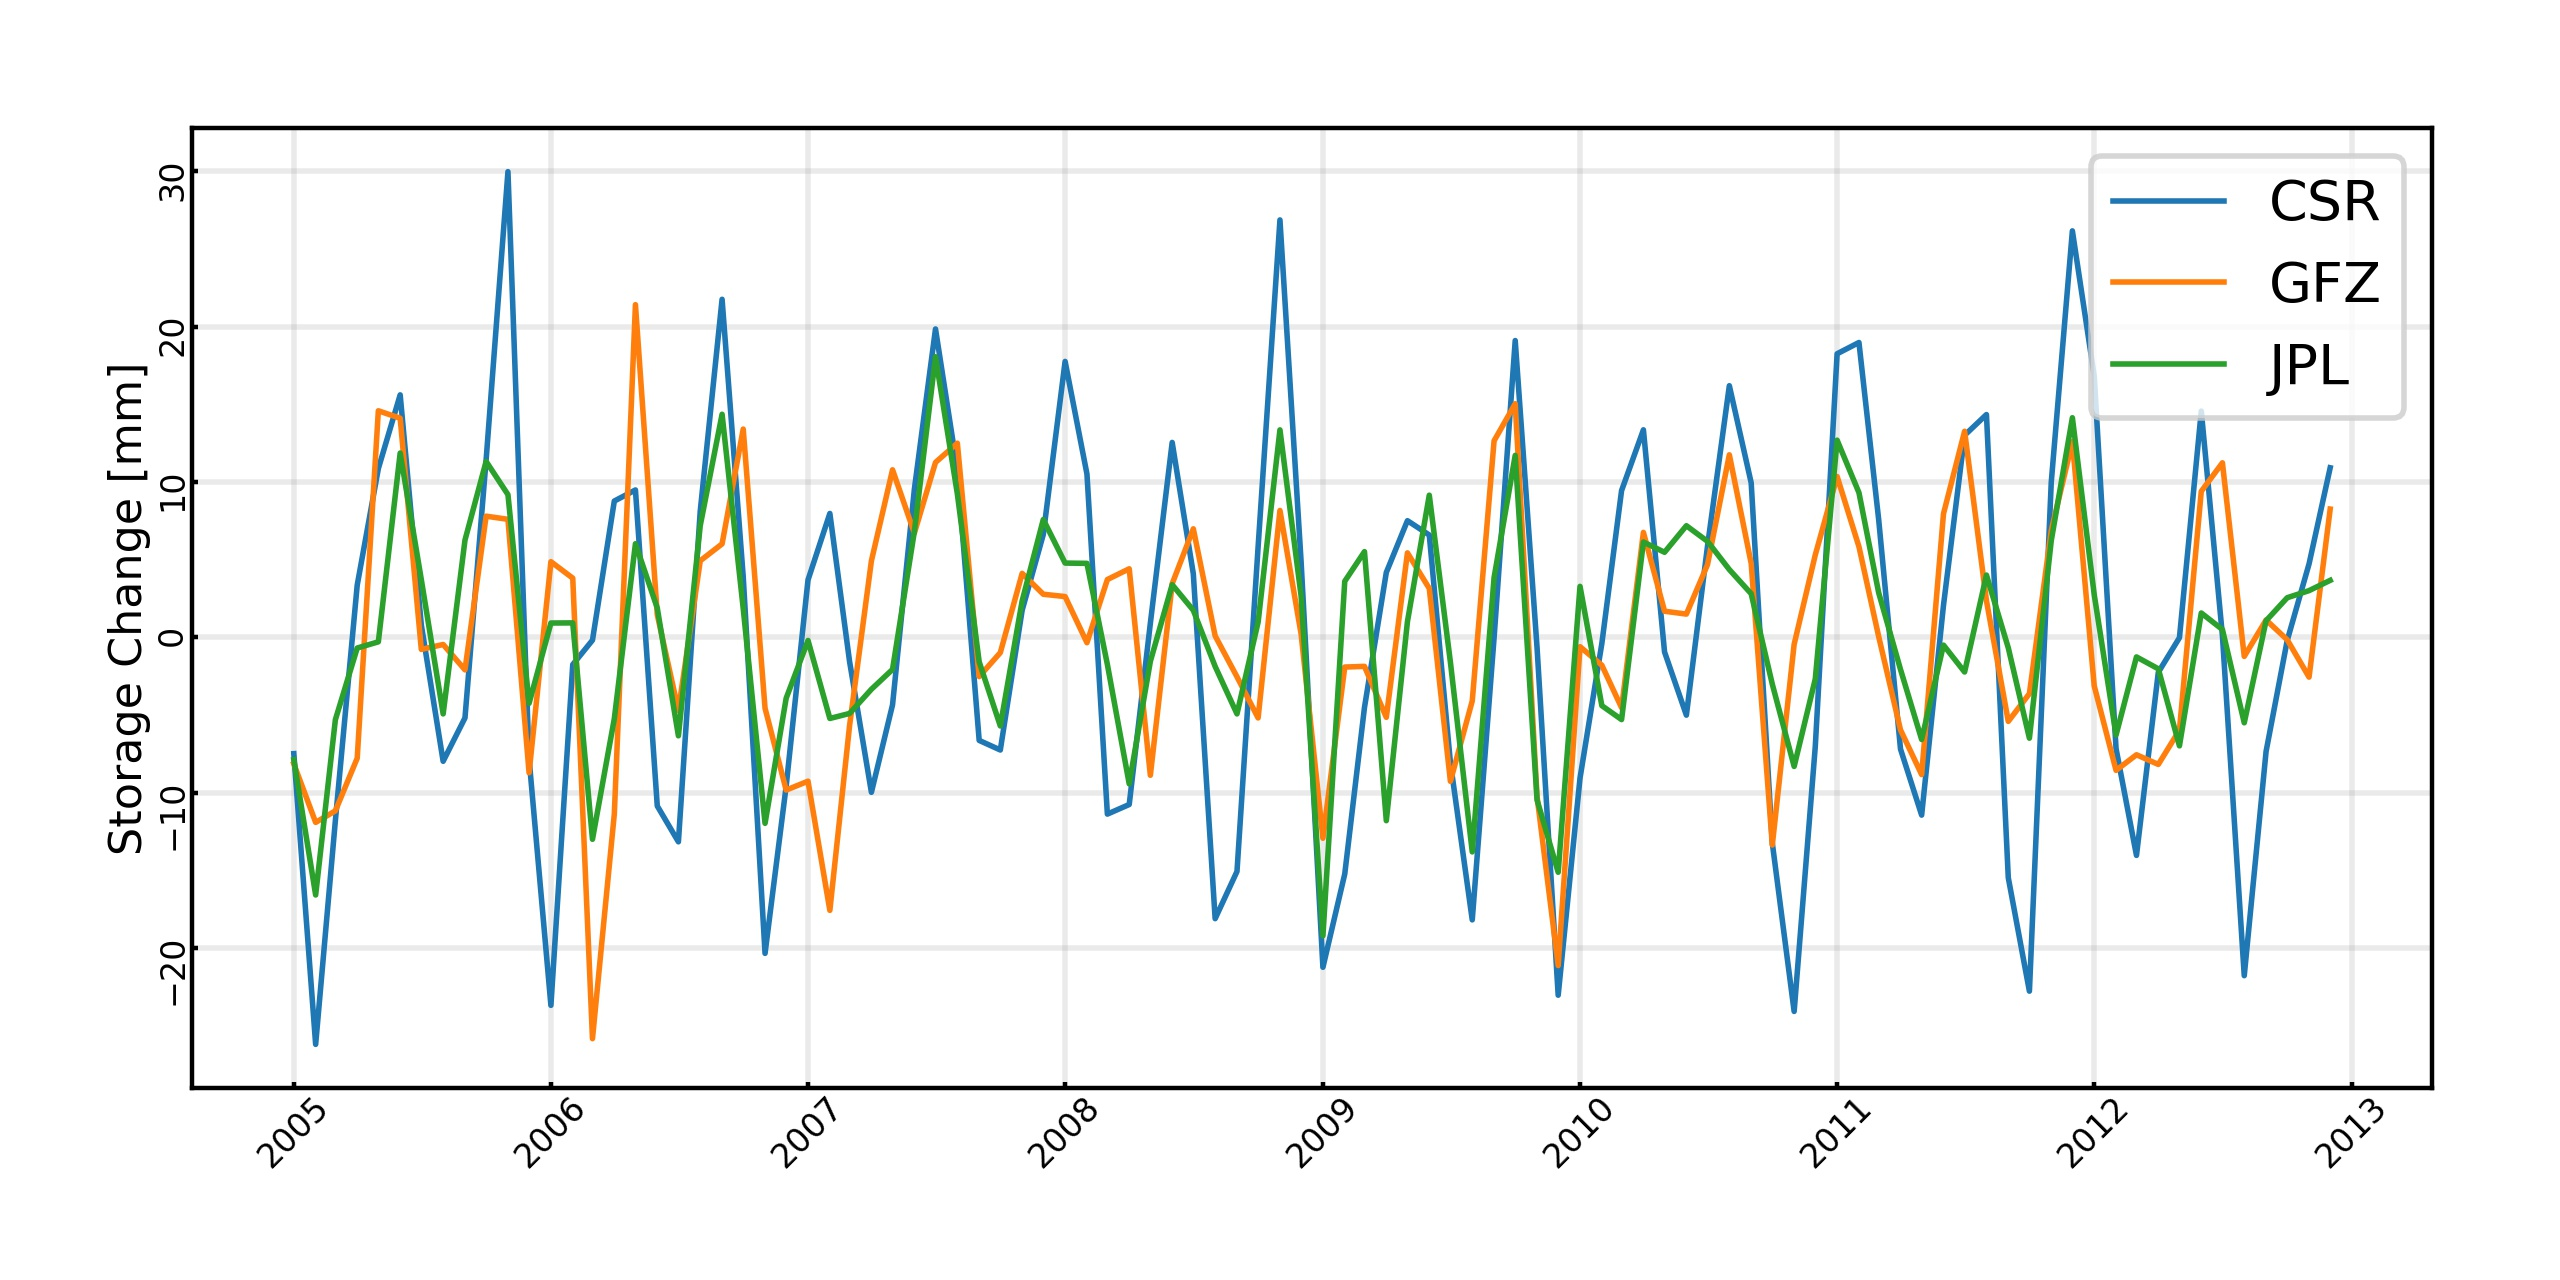
\includegraphics[width=0.8\textwidth]{D:/IHEProjects/TempDev/IHEWAreport/tests/data/area1/fig/fig1c.jpg}%
\caption{GRACE products for Mindanao River Basin}%
\label{figure:fig11}%
\end{figure}

%
In terms of correlation, CMRSET and GLEAM showed the correlation with PCC of 0.82, which means the products are relatively correlated, see Figure \ref{figure:fig12}.%
\linebreak%


\begin{figure}[H]%
\centering%
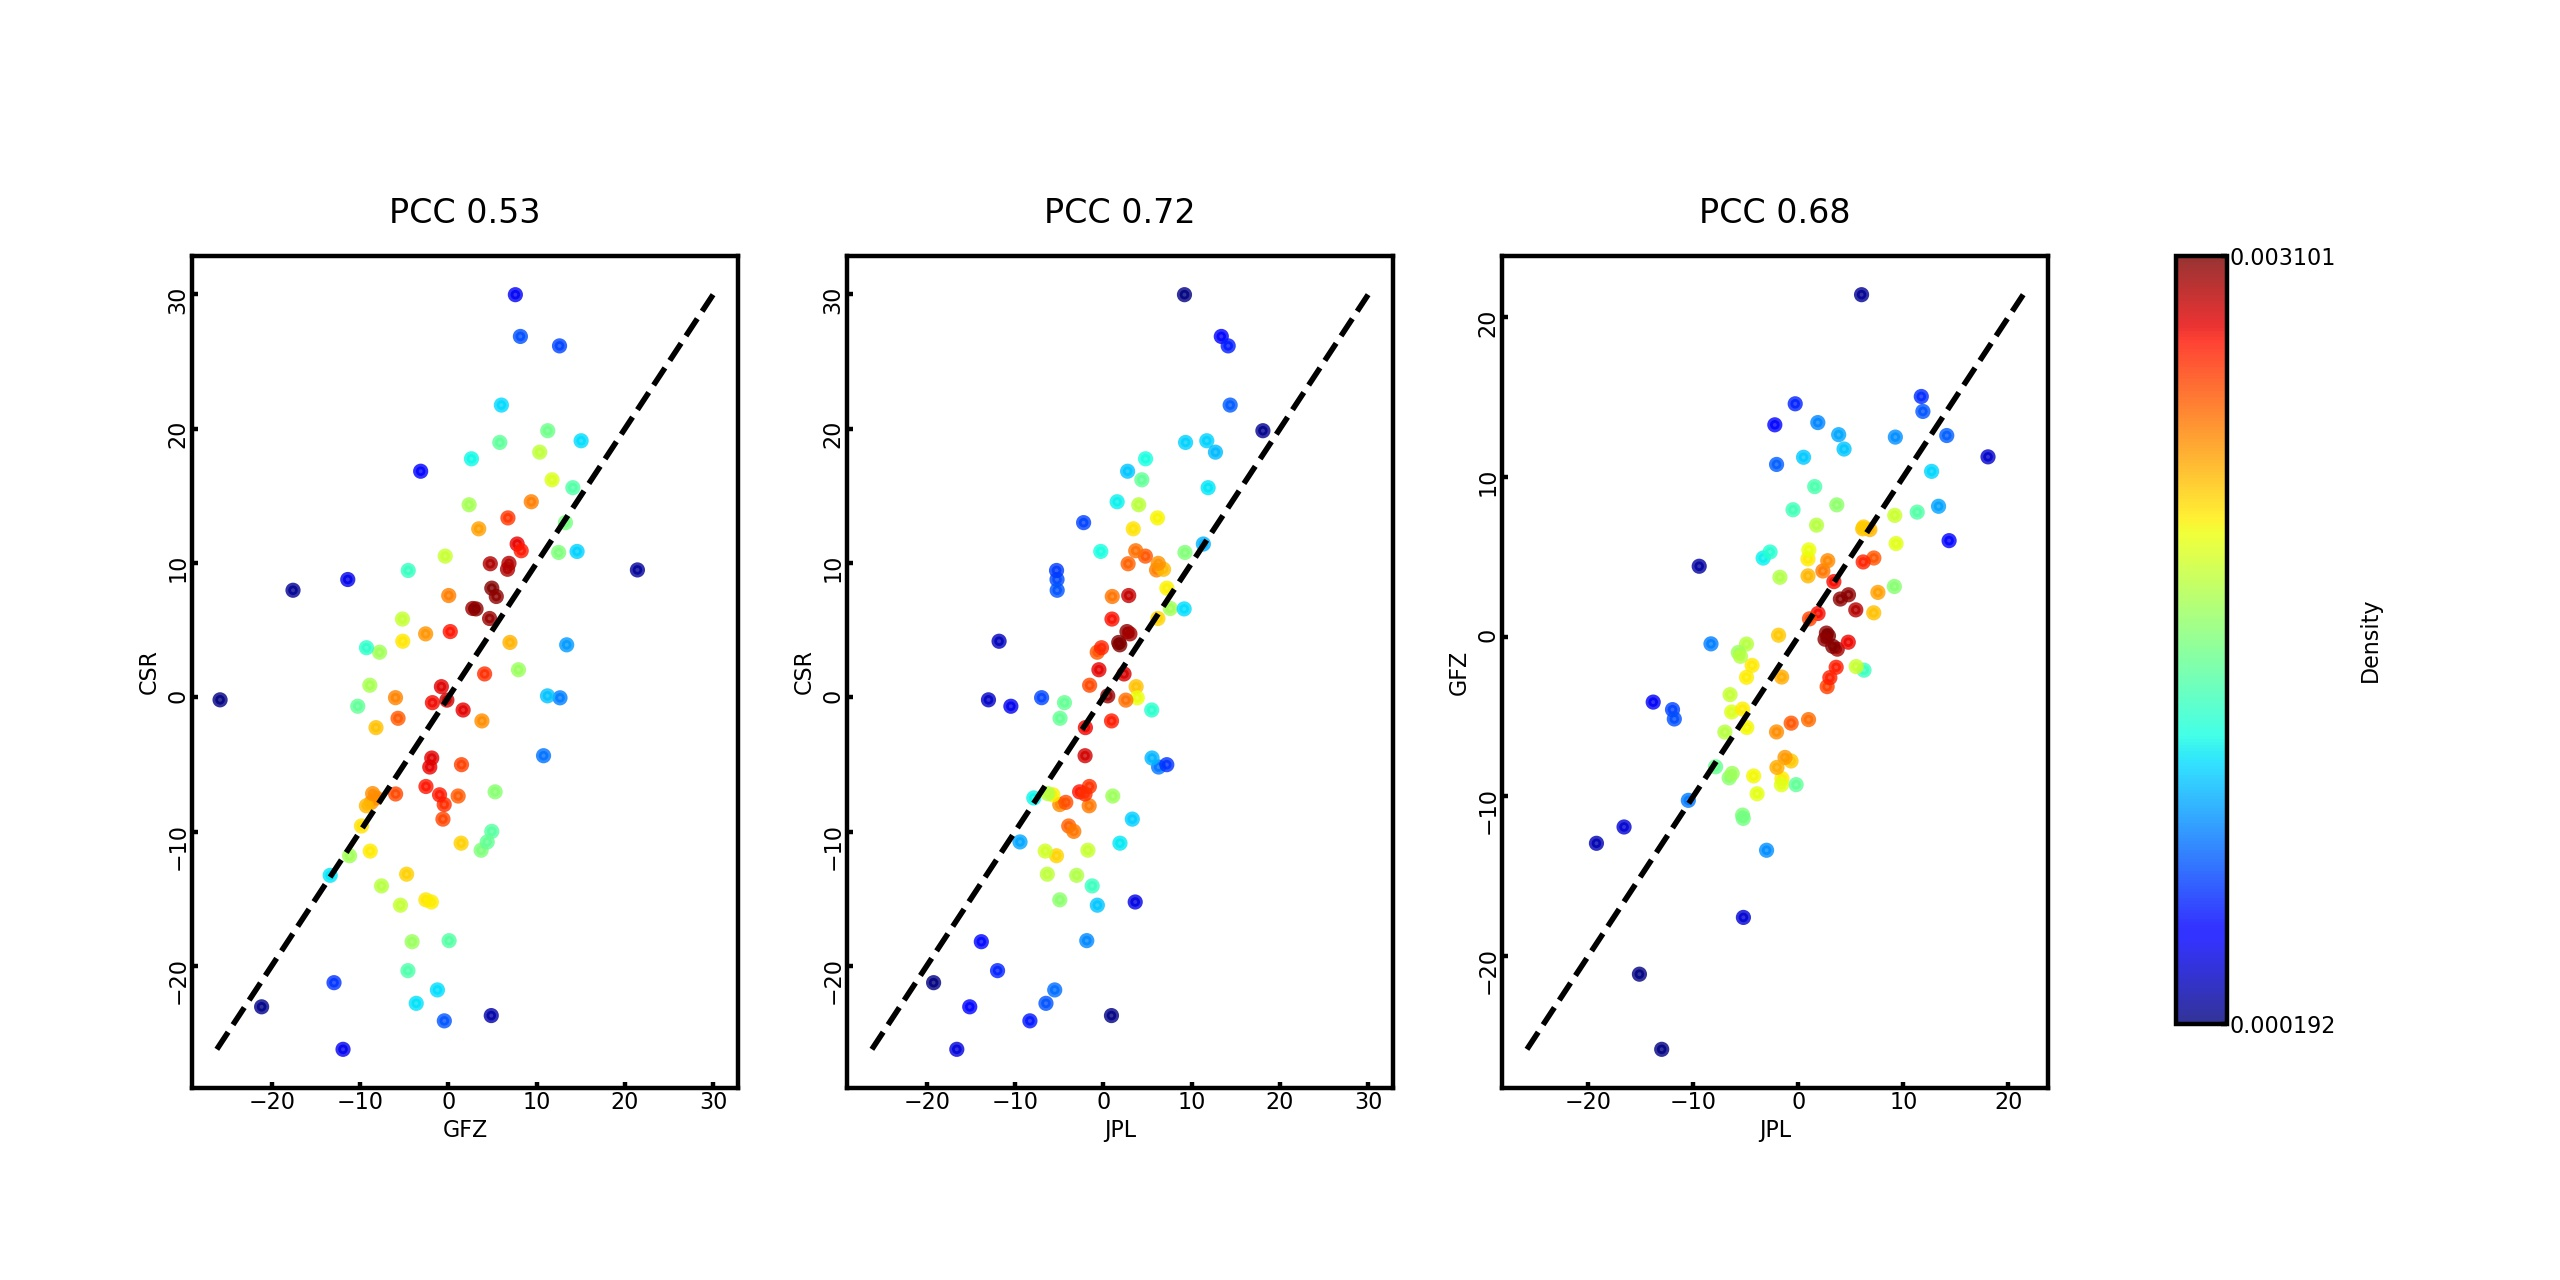
\includegraphics[width=0.8\textwidth]{D:/IHEProjects/TempDev/IHEWAreport/tests/data/area1/fig/fig2c.jpg}%
\caption{Correlation between GRACE products (unit: mm/month)}%
\label{figure:fig12}%
\end{figure}

%
The monthly mean and annual storage change from the products are illustrated in the Figure \ref{figure:fig13} and Figure \ref{figure:fig14}. GFZ solution produced larger volume of storage gain in wet season, CMRSETlost less storage in dry months.%
\linebreak%


\begin{figure}[H]%
\centering%
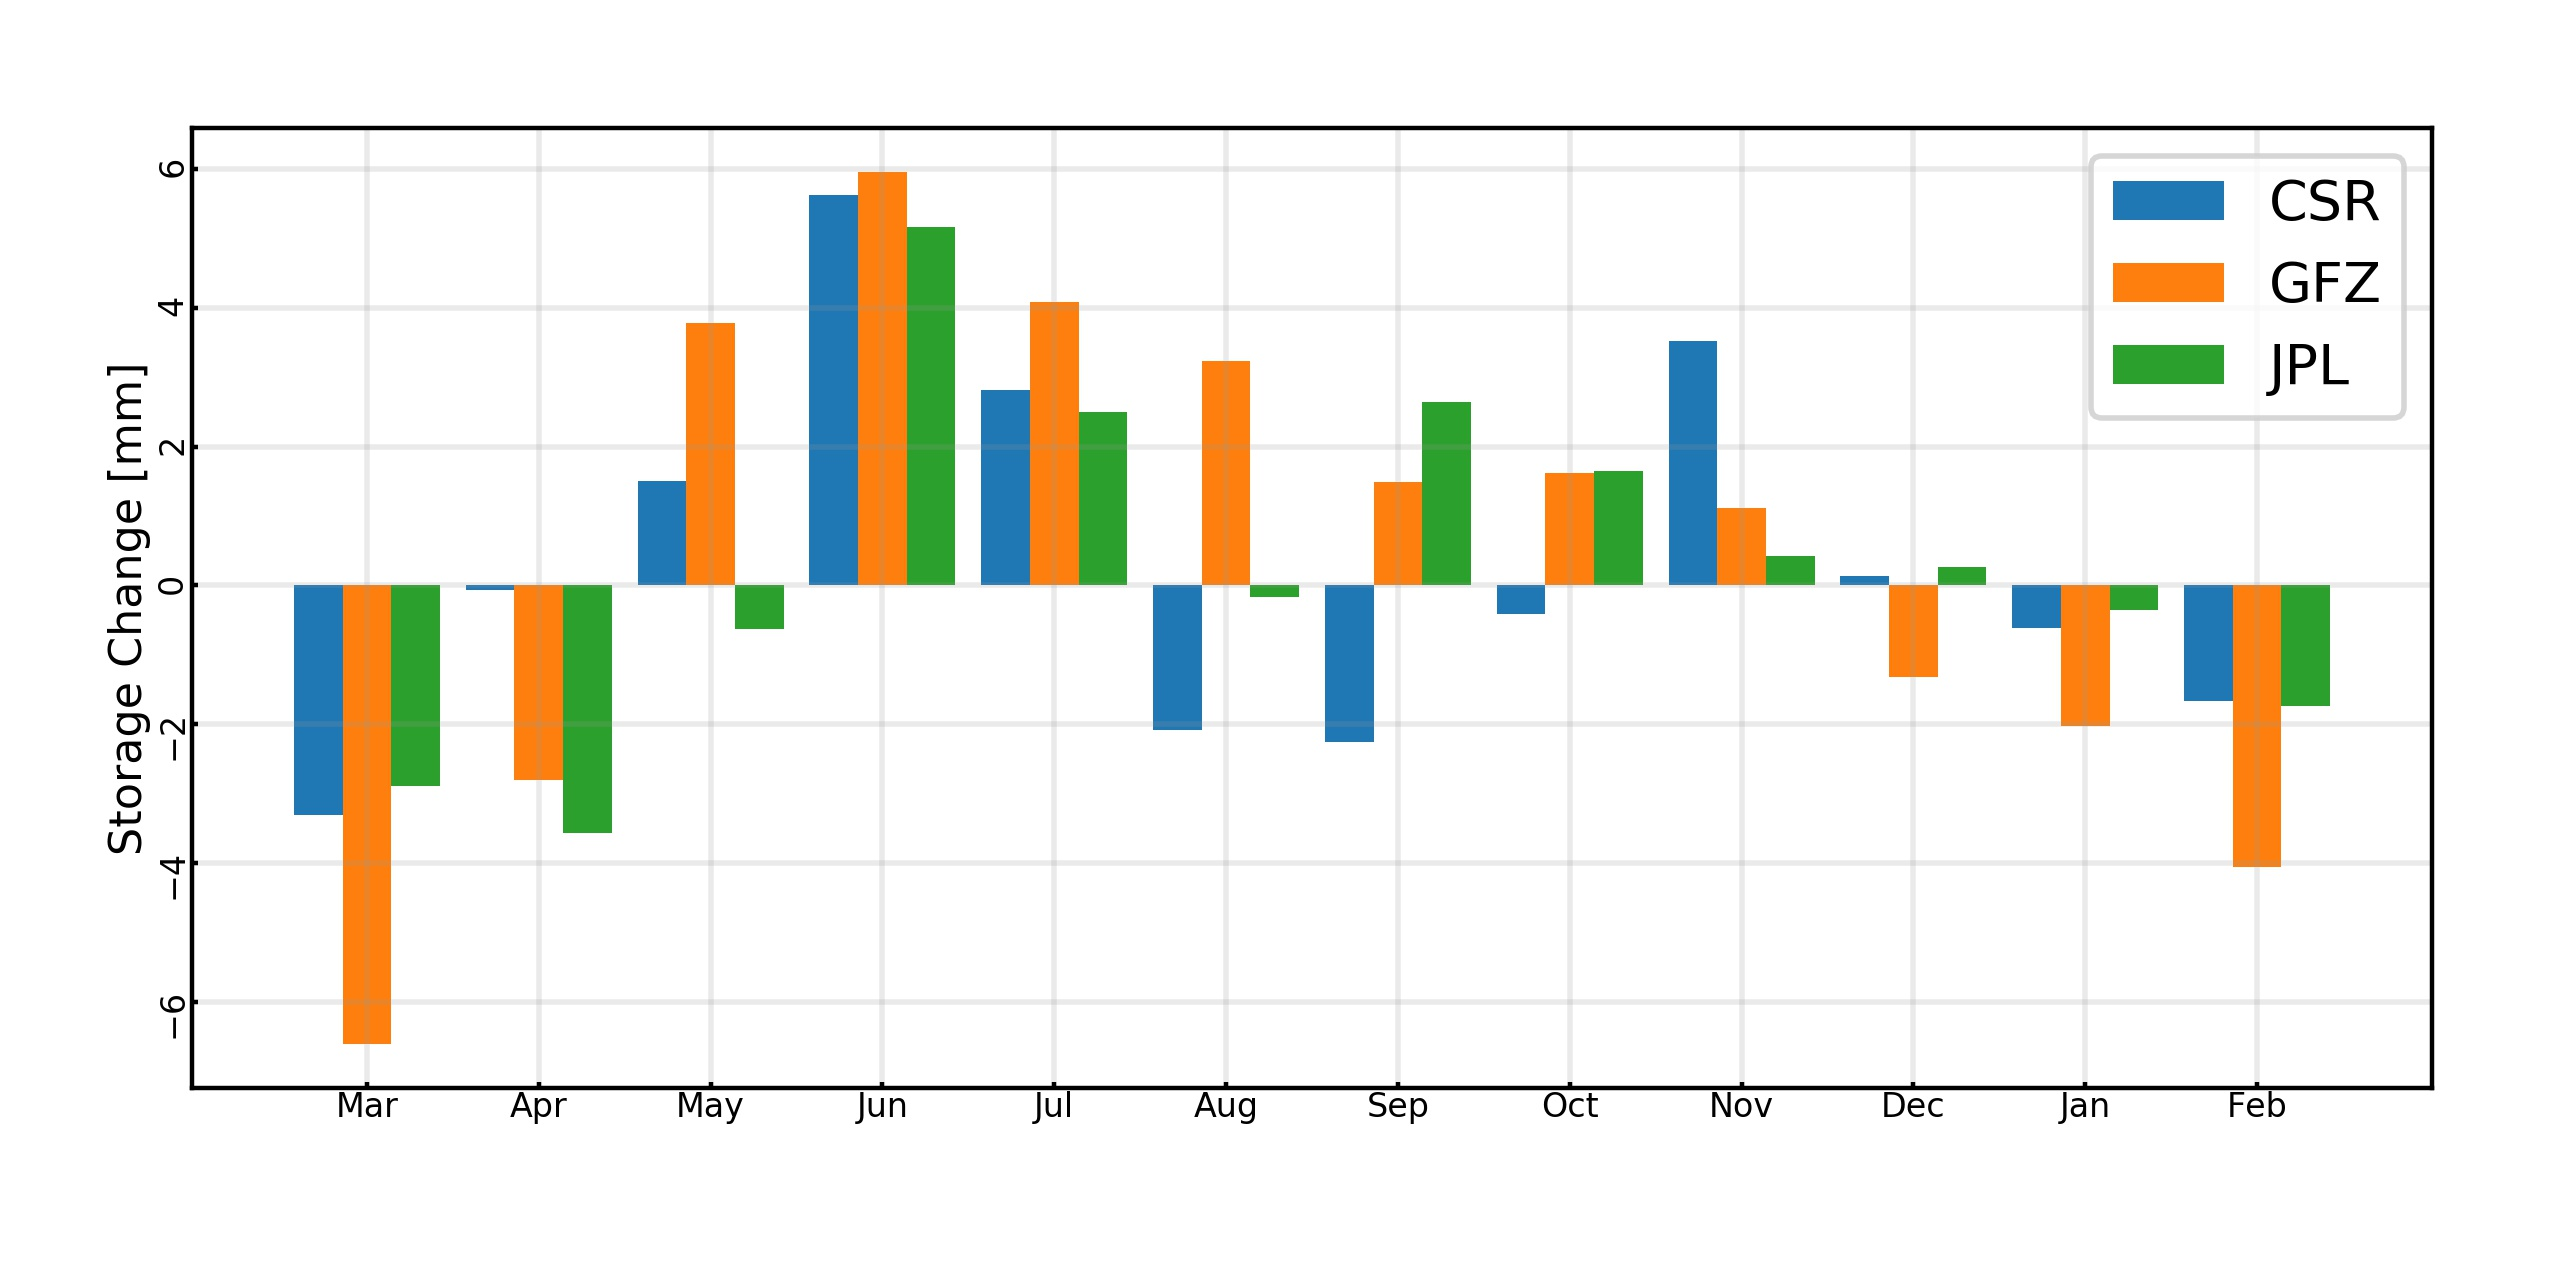
\includegraphics[width=0.8\textwidth]{D:/IHEProjects/TempDev/IHEWAreport/tests/data/area1/fig/fig3c_monthly.jpg}%
\caption{Monthly mean storage change for Mindanao River Basin}%
\label{figure:fig13}%
\end{figure}

%


\begin{figure}[H]%
\centering%
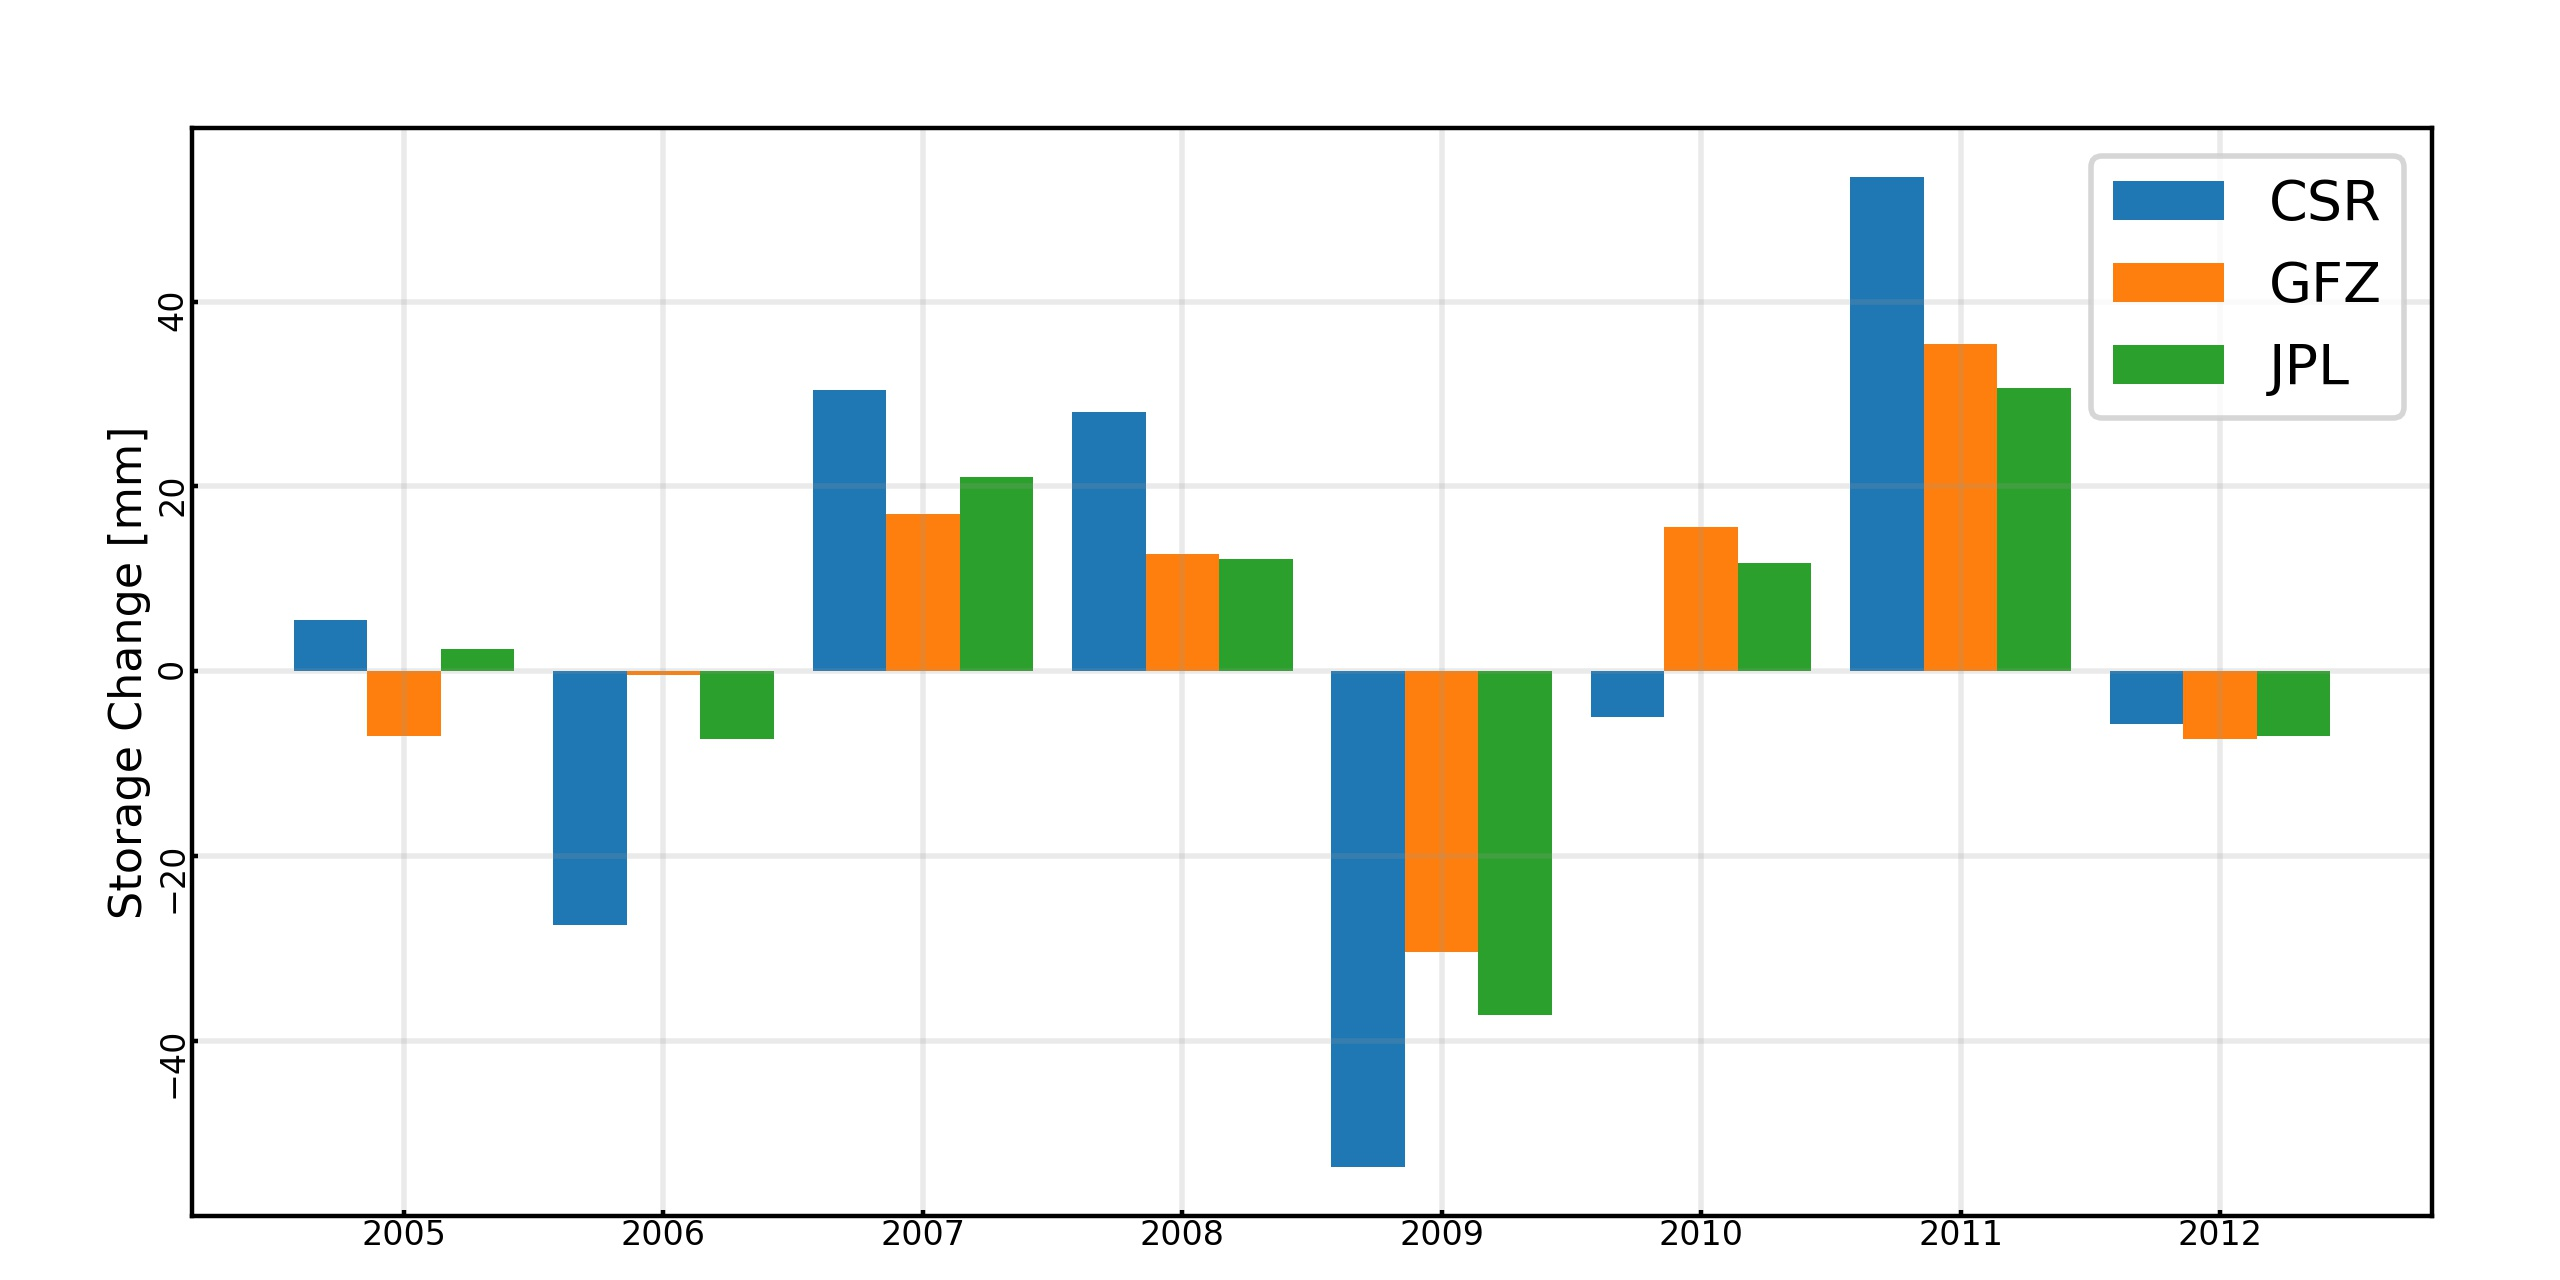
\includegraphics[width=0.8\textwidth]{D:/IHEProjects/TempDev/IHEWAreport/tests/data/area1/fig/fig3c_yearly.jpg}%
\caption{Annual storage change  for Mindanao River Basin}%
\label{figure:fig14}%
\end{figure}

%
\subsection{Runoff comparison}%
\label{subsec:Runoffcomparison}%
Total 60 different possible combinations to compute the water balance for Mindanao River Basin from three precipitation, five evapotranspiration and three GRACE solutions, see Figure \ref{figure:fig15}.%
\linebreak%
\begin{itemize}%
\item%
PCC values vary from {-}0.04 to 0.29. The best performing combination in terms of PCC is GLEAM for evapotranspiration, GPM for precipitation and CSR for change in storage. The second best combination is GLEAM, GPM and GFZ with PCC of 0.26.%
\ldots%
\item%
R2 values are in the range from {-}0.90 to 0.06. The best performing combination in terms of R2 is MOD16A2 for evapotranspiration, GPM for precipitation and CSR for change in storage. The second best combination is CMRSET, GPM and CSR with PCC of 0.05.%
\ldots%
\item%
The minimum RMSE value is 64.44. The best performing combination in terms of RMSE is CMRSET for evapotranspiration, GPM for precipitation and GFZ for change in storage. The second best combination is CMRSET, GPMand JPL with PCC of 64.72.%
\ldots%
\end{itemize}%


\begin{figure}[H]%
\centering%
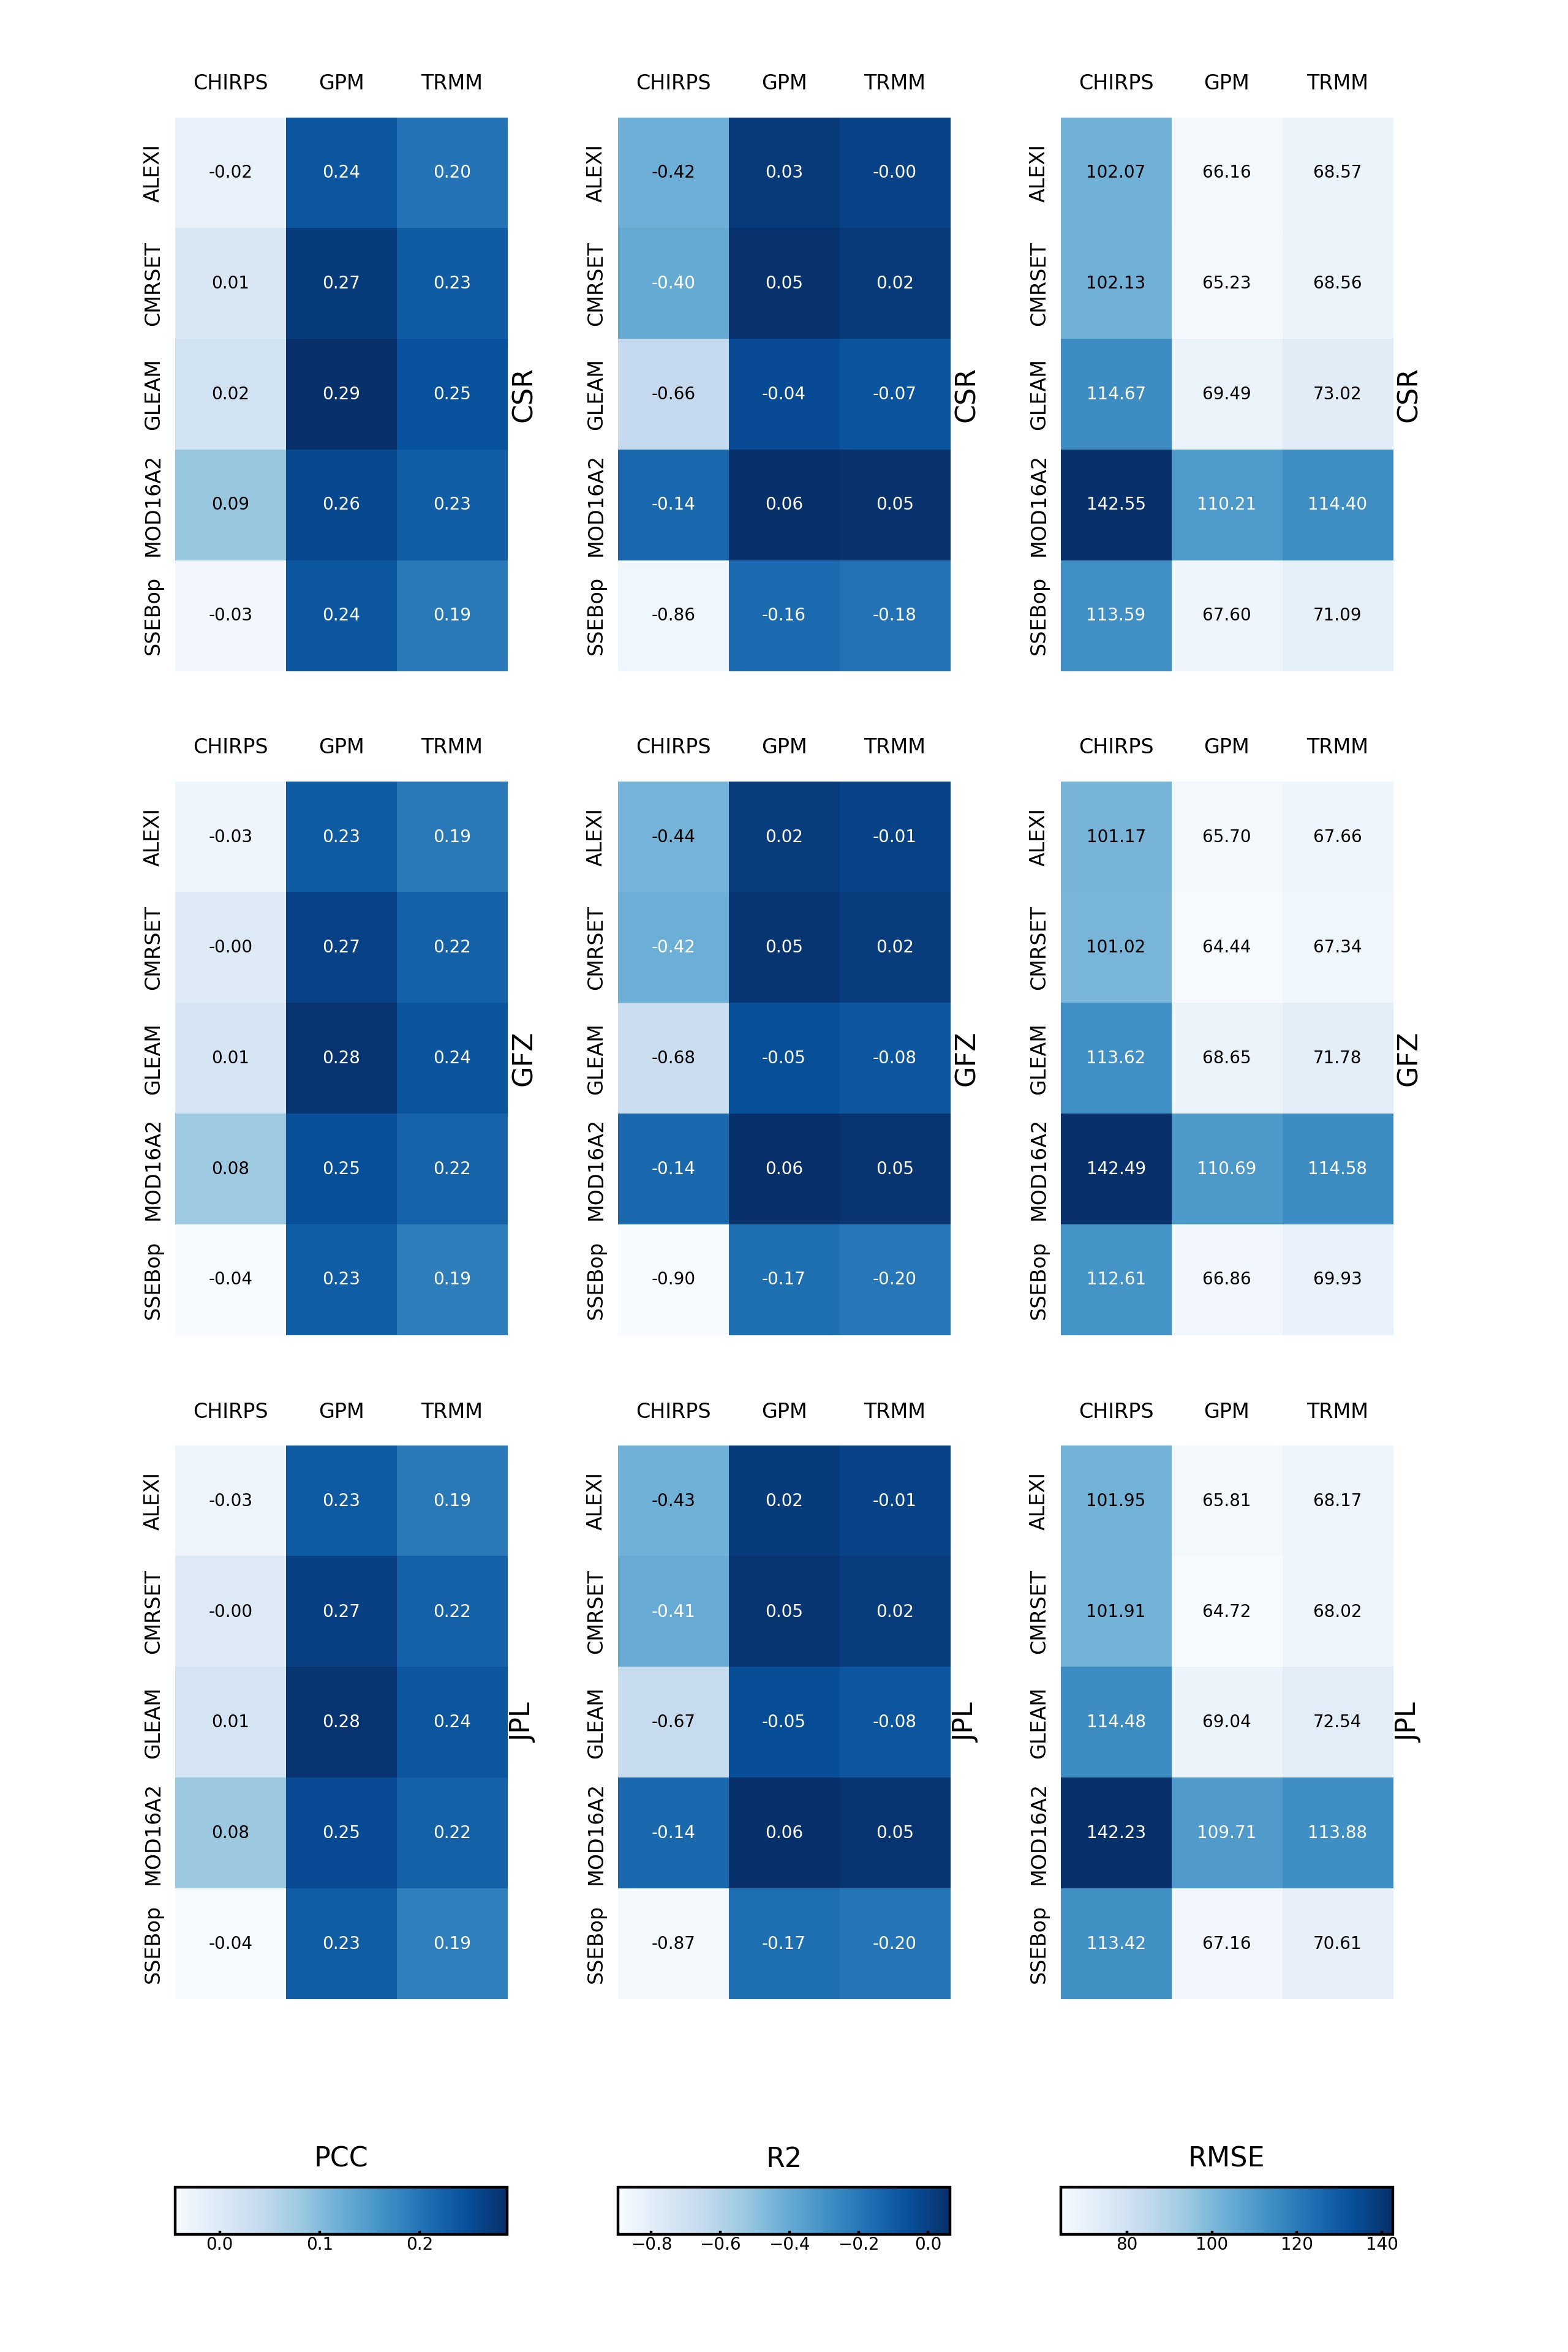
\includegraphics[width=0.8\textwidth]{D:/IHEProjects/TempDev/IHEWAreport/tests/data/area1/fig/fig6.jpg}%
\caption{Performance of different combinations of the remote sensing products to calculate the runoff generated}%
\label{figure:fig15}%
\end{figure}

%
\subsection{Water Balance error}%
\label{subsec:WaterBalanceerror}%
Water balance error is the difference between $P-ET-\Delta S$ and runoff. Figure \ref{figure:fig16} shows the yearly mean water balance error. The combination GPM and MOD16A2 has the lowest error ranging around 1.35\%. However GPM, CMRSET and GFZ has the lowest absolute error 584.81 $Mm^3/year$. The runoff maps of these two are plotted in Figure \ref{figure:fig17}.%
\linebreak%


\begin{figure}[H]%
\centering%
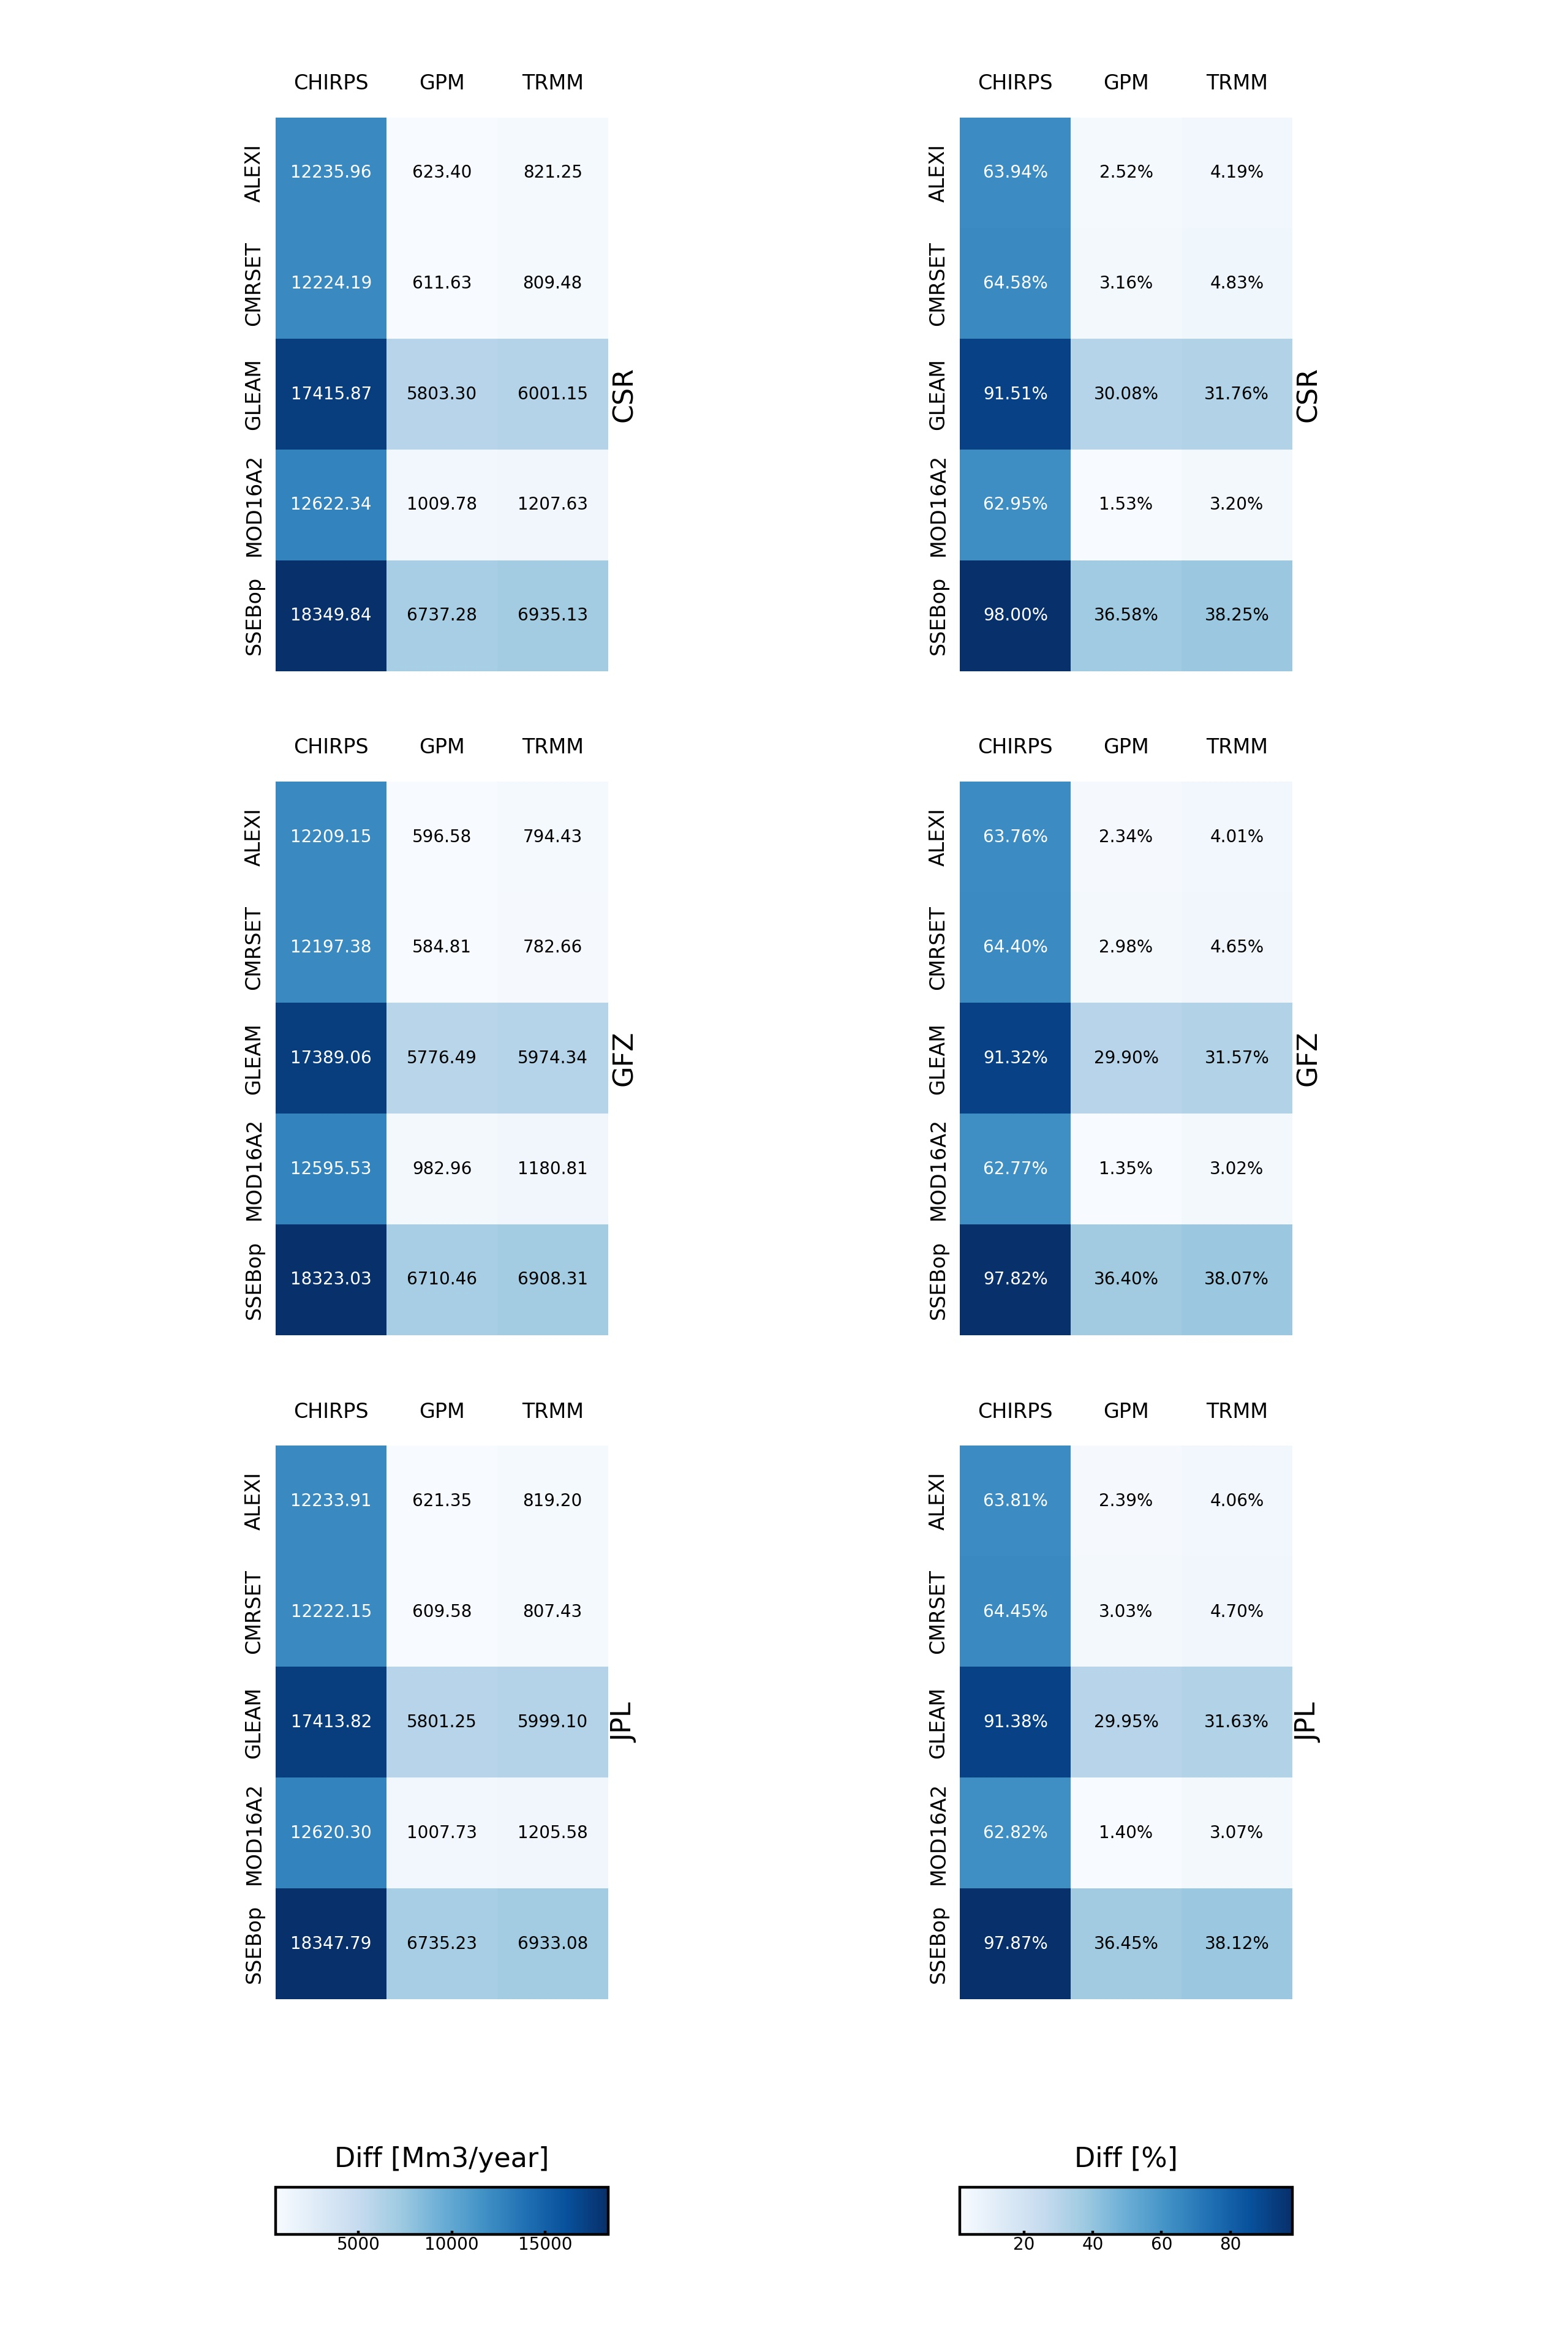
\includegraphics[width=0.8\textwidth]{D:/IHEProjects/TempDev/IHEWAreport/tests/data/area1/fig/fig7.jpg}%
\caption{Water Balance error}%
\label{figure:fig16}%
\end{figure}

%


\begin{figure}[H]%
\begin{subfigure}[c]{0.5\textwidth}%
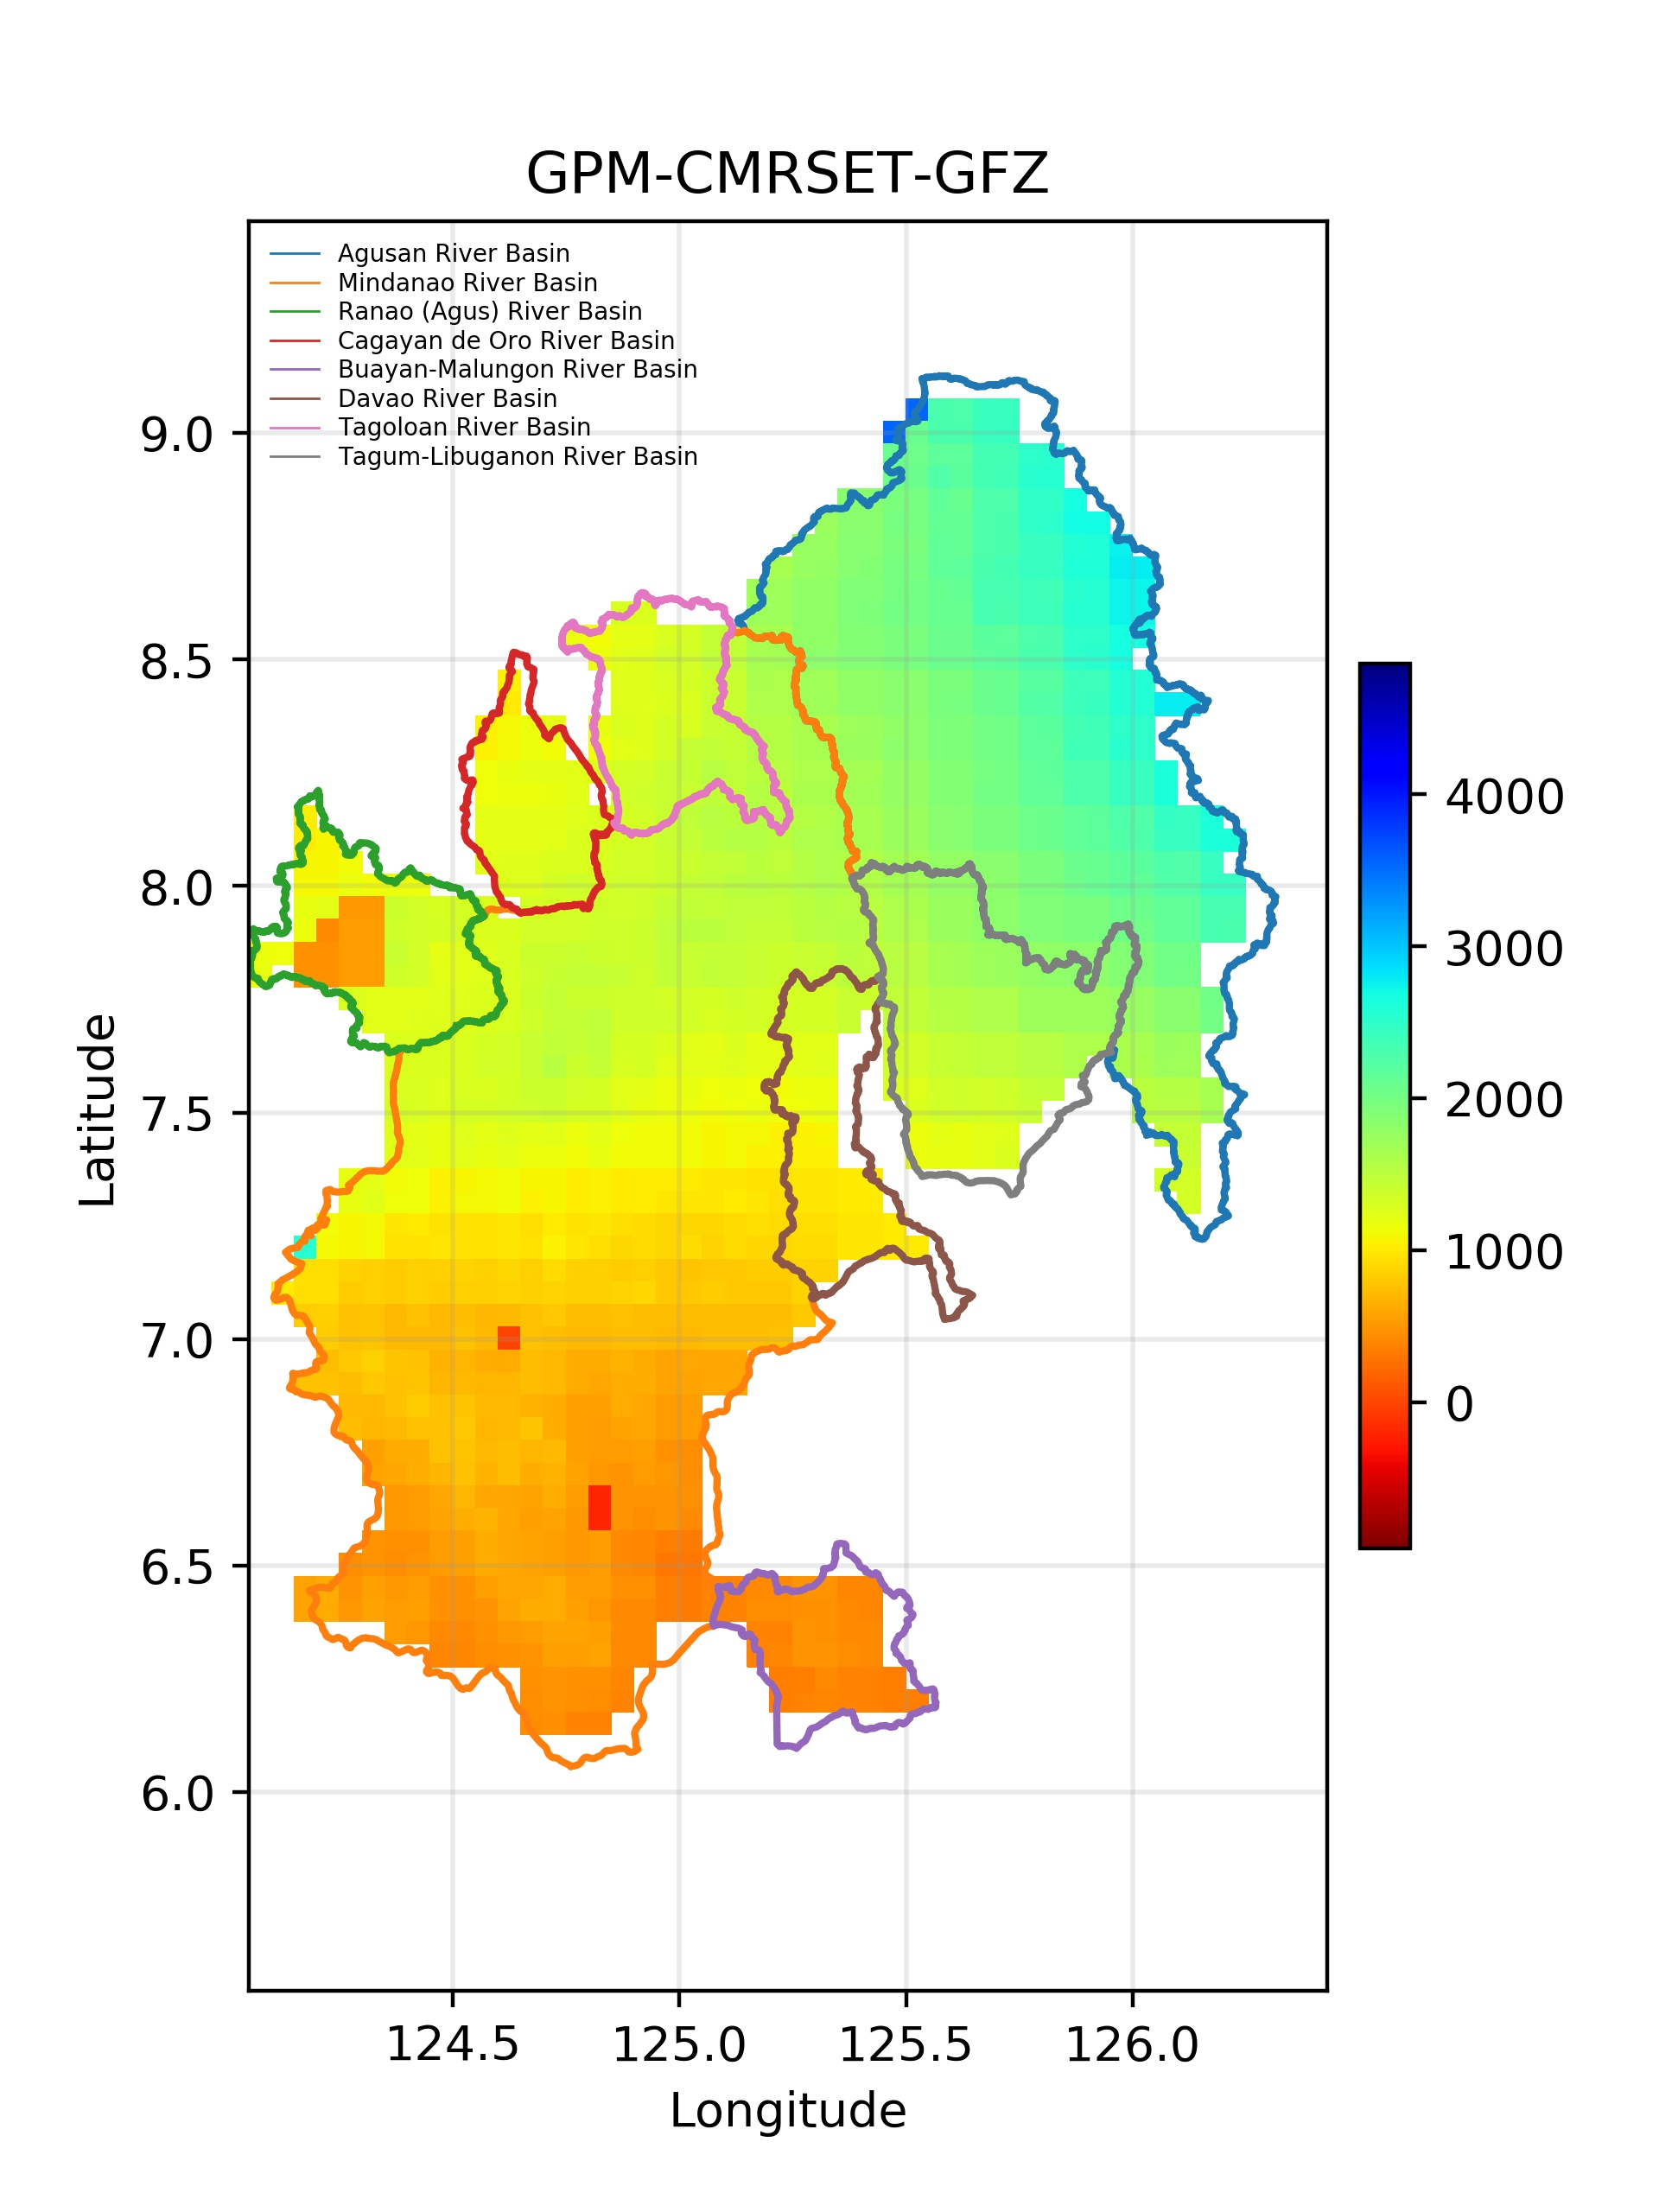
\includegraphics[width=\textwidth]{D:/IHEProjects/TempDev/IHEWAreport/tests/data/area1/fig/fig8_GPM-CMRSET-GFZ.jpg}%
\caption{In term of difference}%
\end{subfigure}%
\begin{subfigure}[c]{0.5\textwidth}%
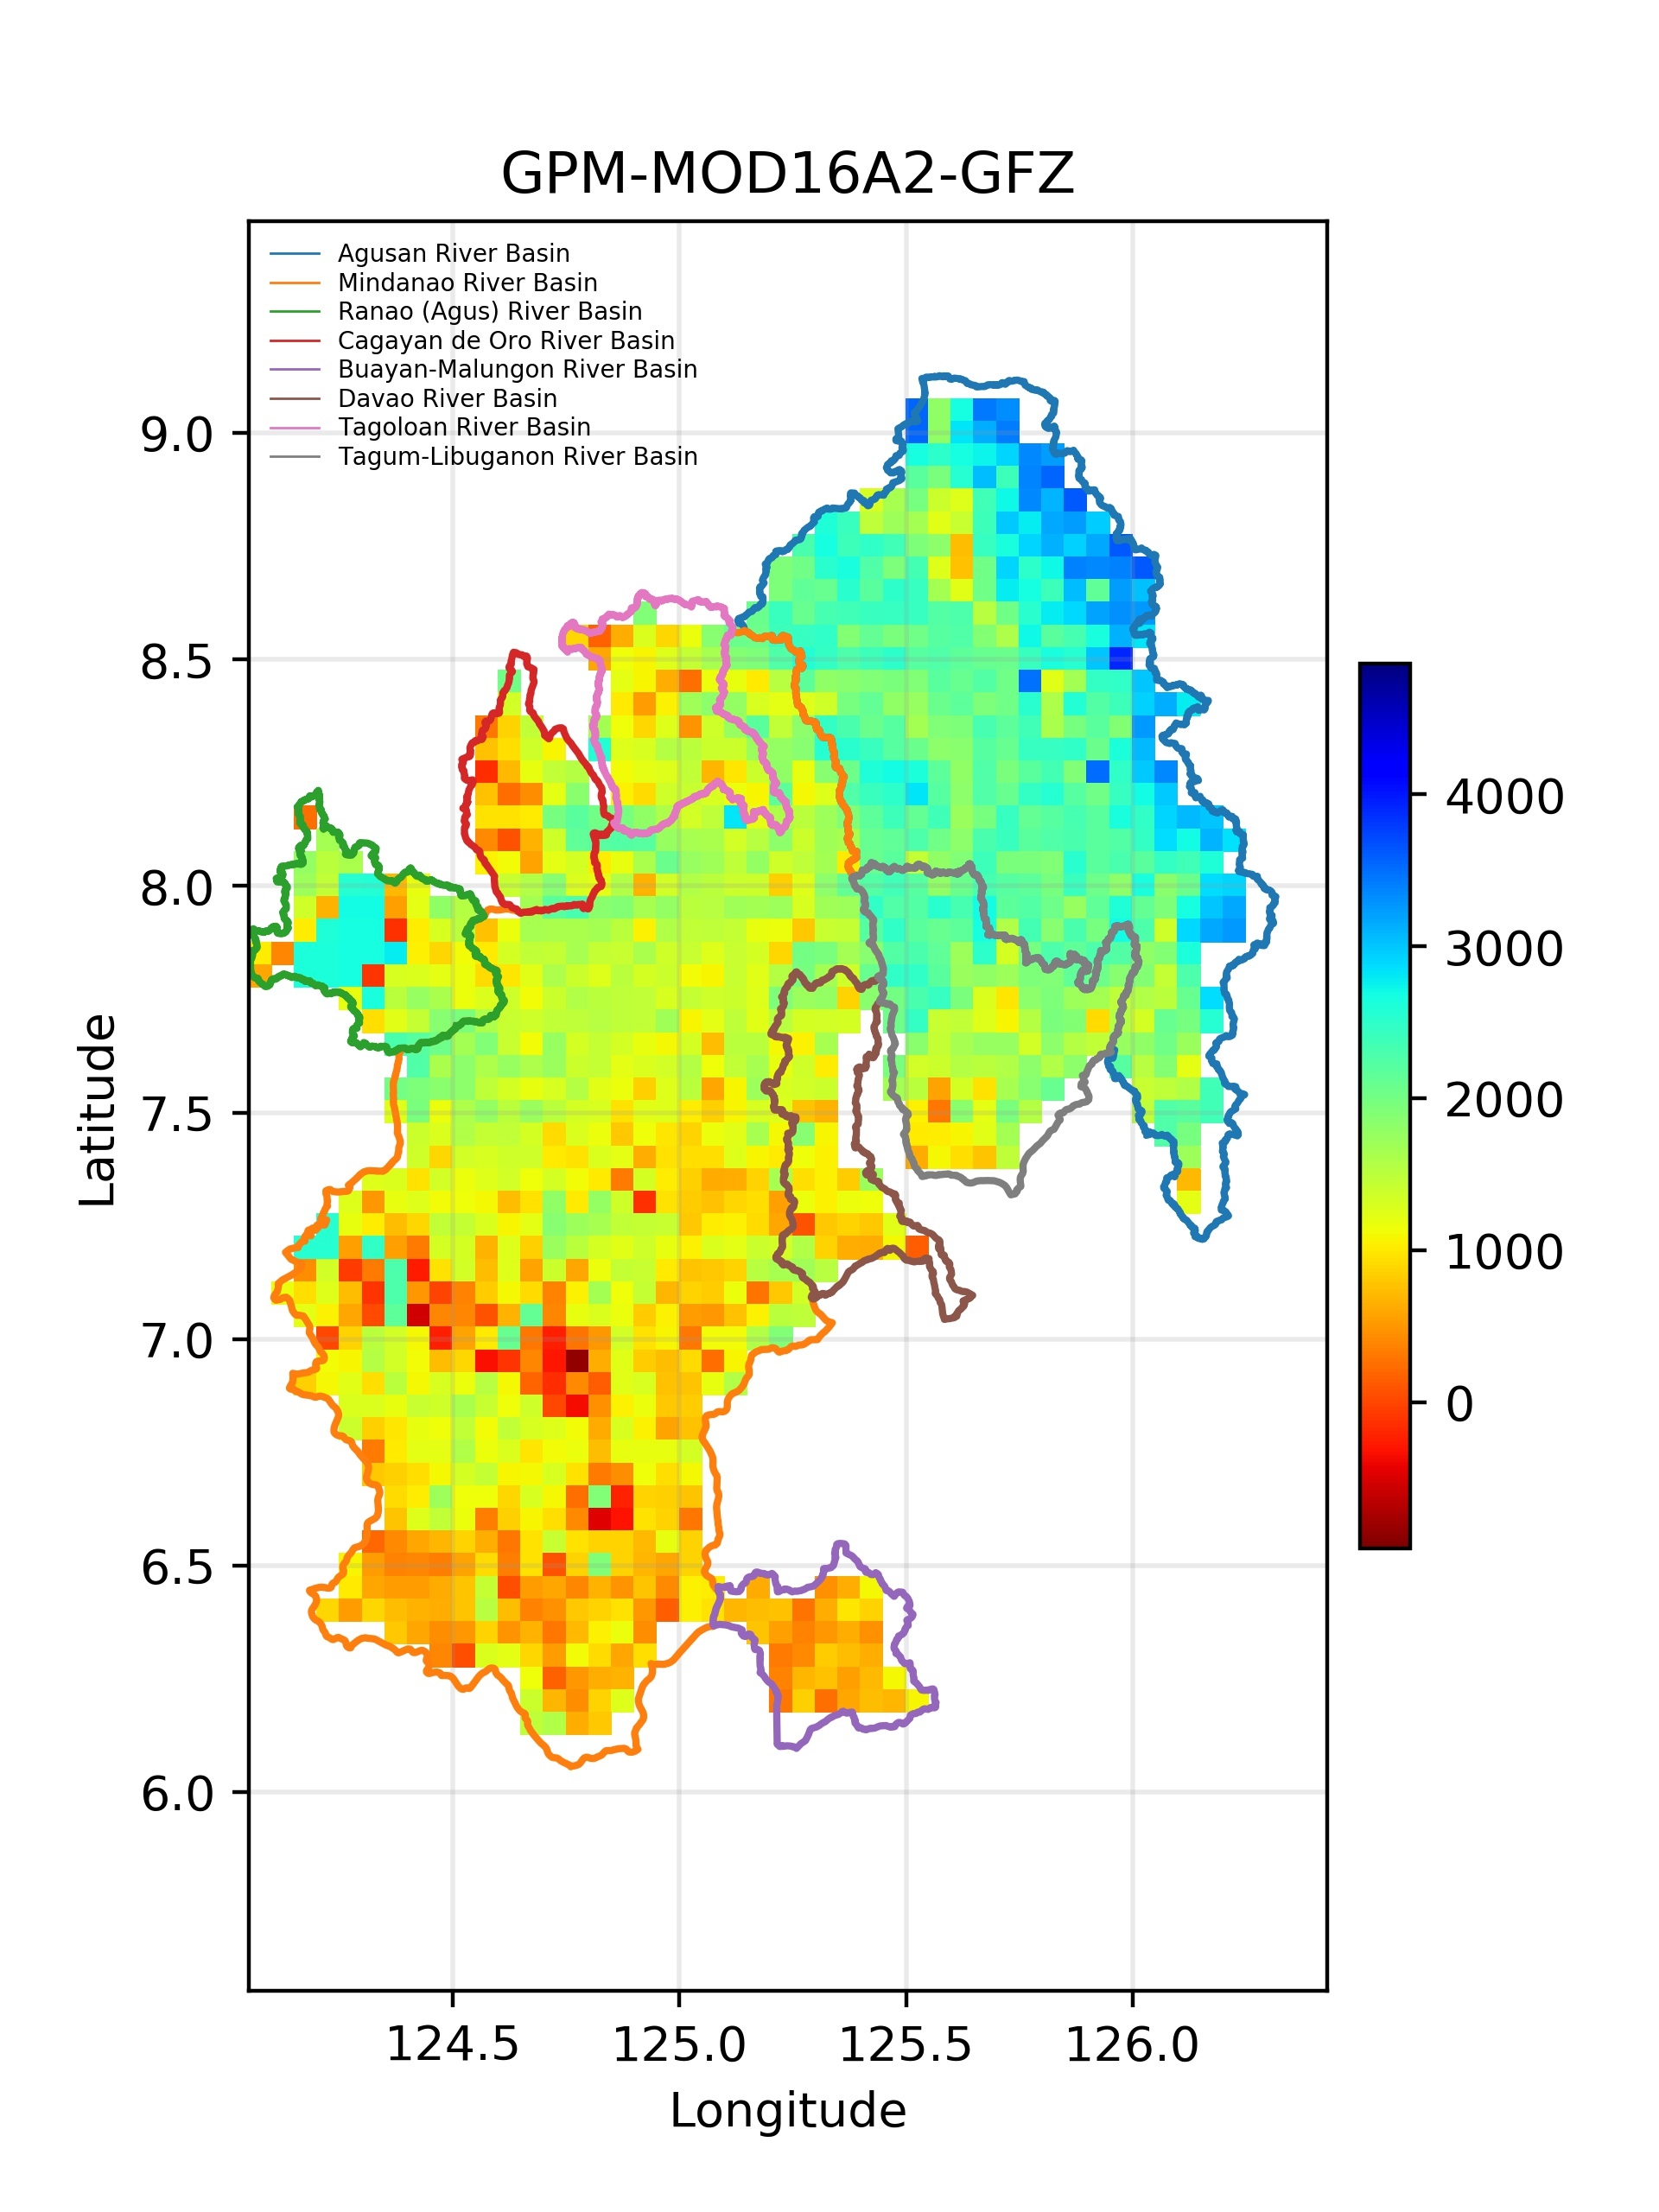
\includegraphics[width=\textwidth]{D:/IHEProjects/TempDev/IHEWAreport/tests/data/area1/fig/fig8_GPM-MOD16A2-GFZ.jpg}%
\caption{In term of difference percentage}%
\end{subfigure}%
\caption{Yearly mean runoff generation map of the best combination}%
\label{figure:fig17}%
\end{figure}

%
\RaggedRight%
\section{Selection of RS products for WA}%
\label{sec:SelectionofRSproductsforWA}%
Due to the PCC and R2 scores are not large enough, which means the correlation is not significant between water balance calculated by different combination and runoff. RMSE is considered as the first criteria to select the best combination of remote sensing products in this study.%
\linebreak%
Thus, evapotranspiration precipitation product GPM, product CMRSET and GRACE solution GFZ are selected for further analysis.%
\linebreak%
Without the full information on other basin transfers, the water balance $P-ET-\Delta S$ is considered in reasonable agreement with outflow. The total observed outflow is 3\% lower than the water balance. The average $P-ET-\Delta S$ is 585 $Mm^3/year$ higher than the sum of flow at outlet. The largest difference is found in the year 2012, which might be attributed to other unaccounted transfers, see Table \ref{table:tab2}.%
\linebreak%
\begin{longtable}{|l|l|l|l|l|l|l|l|}%
\caption{The annual $P-ET-\Delta S$ and $Q$, (unit: $Mm^3/year$)}%
\label{table:tab2}\\%
\hline%
\textbf{Year}&\textbf{P}&\textbf{ET}&\textbf{$\Delta S$}&\textbf{$P-ET-\Delta S$}&\textbf{Q}&\textbf{Diff}&\textbf{\%Diff}\\%
\hline%
\endfirsthead%
\hline%
Year&P&ET&$\Delta S$&$P-ET-\Delta S$&Q&Diff&\%Diff\\%
\hline%
\endhead%
\hline%
\endfoot%
2005&43522&29755&{-}151&13918&13171&747&6\\%
2006&43777&29616&{-}10&14170&16063&{-}1892&{-}12\\%
2007&43650&29405&366&13879&15815&{-}1936&{-}12\\%
2008&59217&29764&273&29180&26240&2940&11\\%
2009&55307&29938&{-}653&26022&25128&894&4\\%
2010&51478&30601&337&20541&16035&4506&28\\%
2011&58280&29171&762&28347&23374&4974&21\\%
2012&49785&30214&{-}158&19730&25283&{-}5553&{-}22\\%
\end{longtable}

%
\newpage%
\section*{References}%
\label{sec:References}%
\addcontentsline{toc}{section}{References}%
\printbibliography[heading=none]

%
\cleardoublepage%
\newpage%
\section*{Annexes}%
\label{sec:Annexes}%
\addcontentsline{toc}{section}{Annexes}%
\RaggedRight%
\subsection*{Remote sensing products}%
\label{subsec:Remotesensingproducts}%
\addcontentsline{toc}{subsection}{Remote sensing products}%
\label{annex:products}%
\subsubsection*{Precipitation}%
\label{ssubsec:Precipitation}%
\textbf{CHIRPS} – The Climate Hazards group Infrared Precipitation with Stations (CHIRPS) dataset, developed by the U.S. Geological Survey Earth Resources Observation and Science Center and Santa Barbara Climate Hazards Group at the University of California is precipitation product based on multiple data sources (Funk et al., 2015). CHIRPS incorporates monthly precipitation climatology (Climate Hazards Group Precipitation Climatology, CHPClim), quasi-global geostationary thermal infrared satellite observations, TRMM product, atmospheric model precipitation fields from the National Oceanic and Atmospheric Administration (NOAA) Climate Forecast System (CFS), and observed precipitation (Funk et al., 2015).%
\linebreak%
\textbf{TRMM} – The Tropical Rainfall Measuring Mission (TRMM), a joint mission of NASA and the Japan Aerospace Exploration Agency, was launched in 1997 to study rainfall for weather and climate research. TRMM Multi-satellite Precipitation Analysis (TMPA) algorithm merges a variety of existing ground- and satellite-based observations to yield high spatial () and temporal esolution (three-hourly instantaneous retrievals) observations with a higher degree of accuracy (Huffman et al., 2007).%
\linebreak%
\textbf{GPM} - NASA/JAXA Global precipitation measurement (GPM) mission in coordination with the Goddard Earth Sciences Data and Information Services Center (GES DISC) is the Integrated Multi-satellite Retrievals for GPM, which merges precipitation estimates from passive microwave (PMW), calibrated infrared (IR) sensors and monthly surface precipitation gauge analysis data to provide half-hourly precipitation estimates on a  grid over the  N-S domain. GPM extend the spatial coverage from its predecessor (TRMM), and also provide improved measurements of precipitation globally (Liu et al., 2017).%
\linebreak

%
\subsubsection*{Evapotranspiration}%
\label{ssubsec:Evapotranspiration}%
\textbf{ALEXI} - Is a coupled two source land surface one dimensional atmospheric boundary layer (ABL) model. The lower boundary conditions for the two source model are provided by thermal IR observations taken at two times during the morning hours.  The ABL model then relates the rise in air temperature above the canopy and the growth of the ABL to the time integrated influx of sensible heating from the surface. (Anderson et al., 2007).%
\linebreak%
\textbf{CMRSET} - CSIRO MODIS Reflectance-based Evapotranspiration (Guerschman et al., 2009).%
\linebreak%
\textbf{GLEAM} - A set of algorithms that separately estimate the different components of land evaporation (or “evapotranspiration”): transpiration, bare-soil evaporation, interception loss, open-water evaporation and sublimation. Additionally, GLEAM provides surface and root-zone soil moisture, potential evaporation and evaporative stress conditions. (Miralles et al., 2011).%
\linebreak%
\textbf{MOD16A2} - Based on surface reflectance from MODIS-Terra and interpolated climate data. The algorithm uses monthly values of the Enhanced Vegetation Index (EVI) and the Global Vegetation Moisture Index (GVMI) derived from the MODIS nadir bidirectional reflectance distribution function – adjusted reflectance product (MOD43B4) to scale Priestley-Taylor potential evapotranspiration derived from the climate surfaces. (Mu et al., 2011).%
\linebreak%
\textbf{SSEBop} - Operational Simplified Surface Energy Balance (Senay et al., 2013).%
\linebreak

%
\subsubsection*{GRACE Solution}%
\label{ssubsec:GRACESolution}%
\textbf{CSR} - Center for Space Research at University of Texas, Austin.%
\linebreak%
\textbf{GFZ} - GeoforschungsZentrum Potsdam%
\linebreak%
\textbf{JPL} - Jet Propulsion Laboratory processing centers (Swenson and Wahr, 2006; Landerer and Swenson, 2012; Swenson, 2012).%
\linebreak

%
\newpage%
\RaggedRight%
\subsection*{The yearly mean $P-ET-\Delta S$ and $Q$, (unit: $Mm^3/year$)}%
\label{subsec:TheyearlymeanP{-}ET{-}DeltaSandQ,(unitMm3/year)}%
\addcontentsline{toc}{subsection}{The yearly mean $P-ET-\Delta S$ and $Q$, (unit: $Mm^3/year$)}%
\begin{longtable}{|l|l|l|l|l|l|l|l|}%
\hline%
\textbf{Combination}&\textbf{P}&\textbf{ET}&\textbf{$\Delta S$}&\textbf{$P-ET-\Delta S$}&\textbf{Q}&\textbf{Diff}&\textbf{\%Diff}\\%
\hline%
\endfirsthead%
\hline%
Combination&P&ET&$\Delta S$&$P-ET-\Delta S$&Q&Diff&\%Diff\\%
\hline%
\endhead%
\hline%
\endfoot%
CHIRPS-ALEXI-CSR&62240&29796&69&32375&20139&12236&64\\%
GPM-ALEXI-CSR&50627&29796&69&20762&20139&623&3\\%
TRMM-ALEXI-CSR&50825&29796&69&20960&20139&821&4\\%
CHIRPS-CMRSET-CSR&62240&29808&69&32363&20139&12224&65\\%
GPM-CMRSET-CSR&50627&29808&69&20750&20139&612&3\\%
TRMM-CMRSET-CSR&50825&29808&69&20948&20139&809&5\\%
CHIRPS-GLEAM-CSR&62240&24616&69&37554&20139&17416&92\\%
GPM-GLEAM-CSR&50627&24616&69&25942&20139&5803&30\\%
TRMM-GLEAM-CSR&50825&24616&69&26140&20139&6001&32\\%
CHIRPS-MOD16A2-CSR&62240&29410&69&32761&20139&12622&63\\%
GPM-MOD16A2-CSR&50627&29410&69&21148&20139&1010&2\\%
TRMM-MOD16A2-CSR&50825&29410&69&21346&20139&1208&3\\%
CHIRPS-SSEBop-CSR&62240&23682&69&38488&20139&18350&98\\%
GPM-SSEBop-CSR&50627&23682&69&26876&20139&6737&37\\%
TRMM-SSEBop-CSR&50825&23682&69&27074&20139&6935&38\\%
CHIRPS-ALEXI-GFZ&62240&29796&96&32348&20139&12209&64\\%
GPM-ALEXI-GFZ&50627&29796&96&20735&20139&597&2\\%
TRMM-ALEXI-GFZ&50825&29796&96&20933&20139&794&4\\%
CHIRPS-CMRSET-GFZ&62240&29808&96&32336&20139&12197&64\\%
GPM-CMRSET-GFZ&50627&29808&96&20723&20139&585&3\\%
TRMM-CMRSET-GFZ&50825&29808&96&20921&20139&783&5\\%
CHIRPS-GLEAM-GFZ&62240&24616&96&37528&20139&17389&91\\%
GPM-GLEAM-GFZ&50627&24616&96&25915&20139&5776&30\\%
TRMM-GLEAM-GFZ&50825&24616&96&26113&20139&5974&32\\%
CHIRPS-MOD16A2-GFZ&62240&29410&96&32734&20139&12596&63\\%
GPM-MOD16A2-GFZ&50627&29410&96&21122&20139&983&1\\%
TRMM-MOD16A2-GFZ&50825&29410&96&21319&20139&1181&3\\%
CHIRPS-SSEBop-GFZ&62240&23682&96&38462&20139&18323&98\\%
GPM-SSEBop-GFZ&50627&23682&96&26849&20139&6710&36\\%
TRMM-SSEBop-GFZ&50825&23682&96&27047&20139&6908&38\\%
CHIRPS-ALEXI-JPL&62240&29796&71&32373&20139&12234&64\\%
GPM-ALEXI-JPL&50627&29796&71&20760&20139&621&2\\%
TRMM-ALEXI-JPL&50825&29796&71&20958&20139&819&4\\%
CHIRPS-CMRSET-JPL&62240&29808&71&32361&20139&12222&64\\%
GPM-CMRSET-JPL&50627&29808&71&20748&20139&610&3\\%
TRMM-CMRSET-JPL&50825&29808&71&20946&20139&807&5\\%
CHIRPS-GLEAM-JPL&62240&24616&71&37552&20139&17414&91\\%
GPM-GLEAM-JPL&50627&24616&71&25940&20139&5801&30\\%
TRMM-GLEAM-JPL&50825&24616&71&26138&20139&5999&32\\%
CHIRPS-MOD16A2-JPL&62240&29410&71&32759&20139&12620&63\\%
GPM-MOD16A2-JPL&50627&29410&71&21146&20139&1008&1\\%
TRMM-MOD16A2-JPL&50825&29410&71&21344&20139&1206&3\\%
CHIRPS-SSEBop-JPL&62240&23682&71&38486&20139&18348&98\\%
GPM-SSEBop-JPL&50627&23682&71&26874&20139&6735&36\\%
TRMM-SSEBop-JPL&50825&23682&71&27072&20139&6933&38\\%
\end{longtable}

%
\newpage%
\RaggedRight%
\subsection*{The water balance $P-ET-\Delta S$ and discharge Q, (unit: mm/month)}%
\label{subsec:ThewaterbalanceP{-}ET{-}DeltaSanddischargeQ,(unitmm/month)}%
\addcontentsline{toc}{subsection}{The water balance $P-ET-\Delta S$ and discharge Q, (unit: mm/month)}%


\begin{figure}[H]%
\centering%
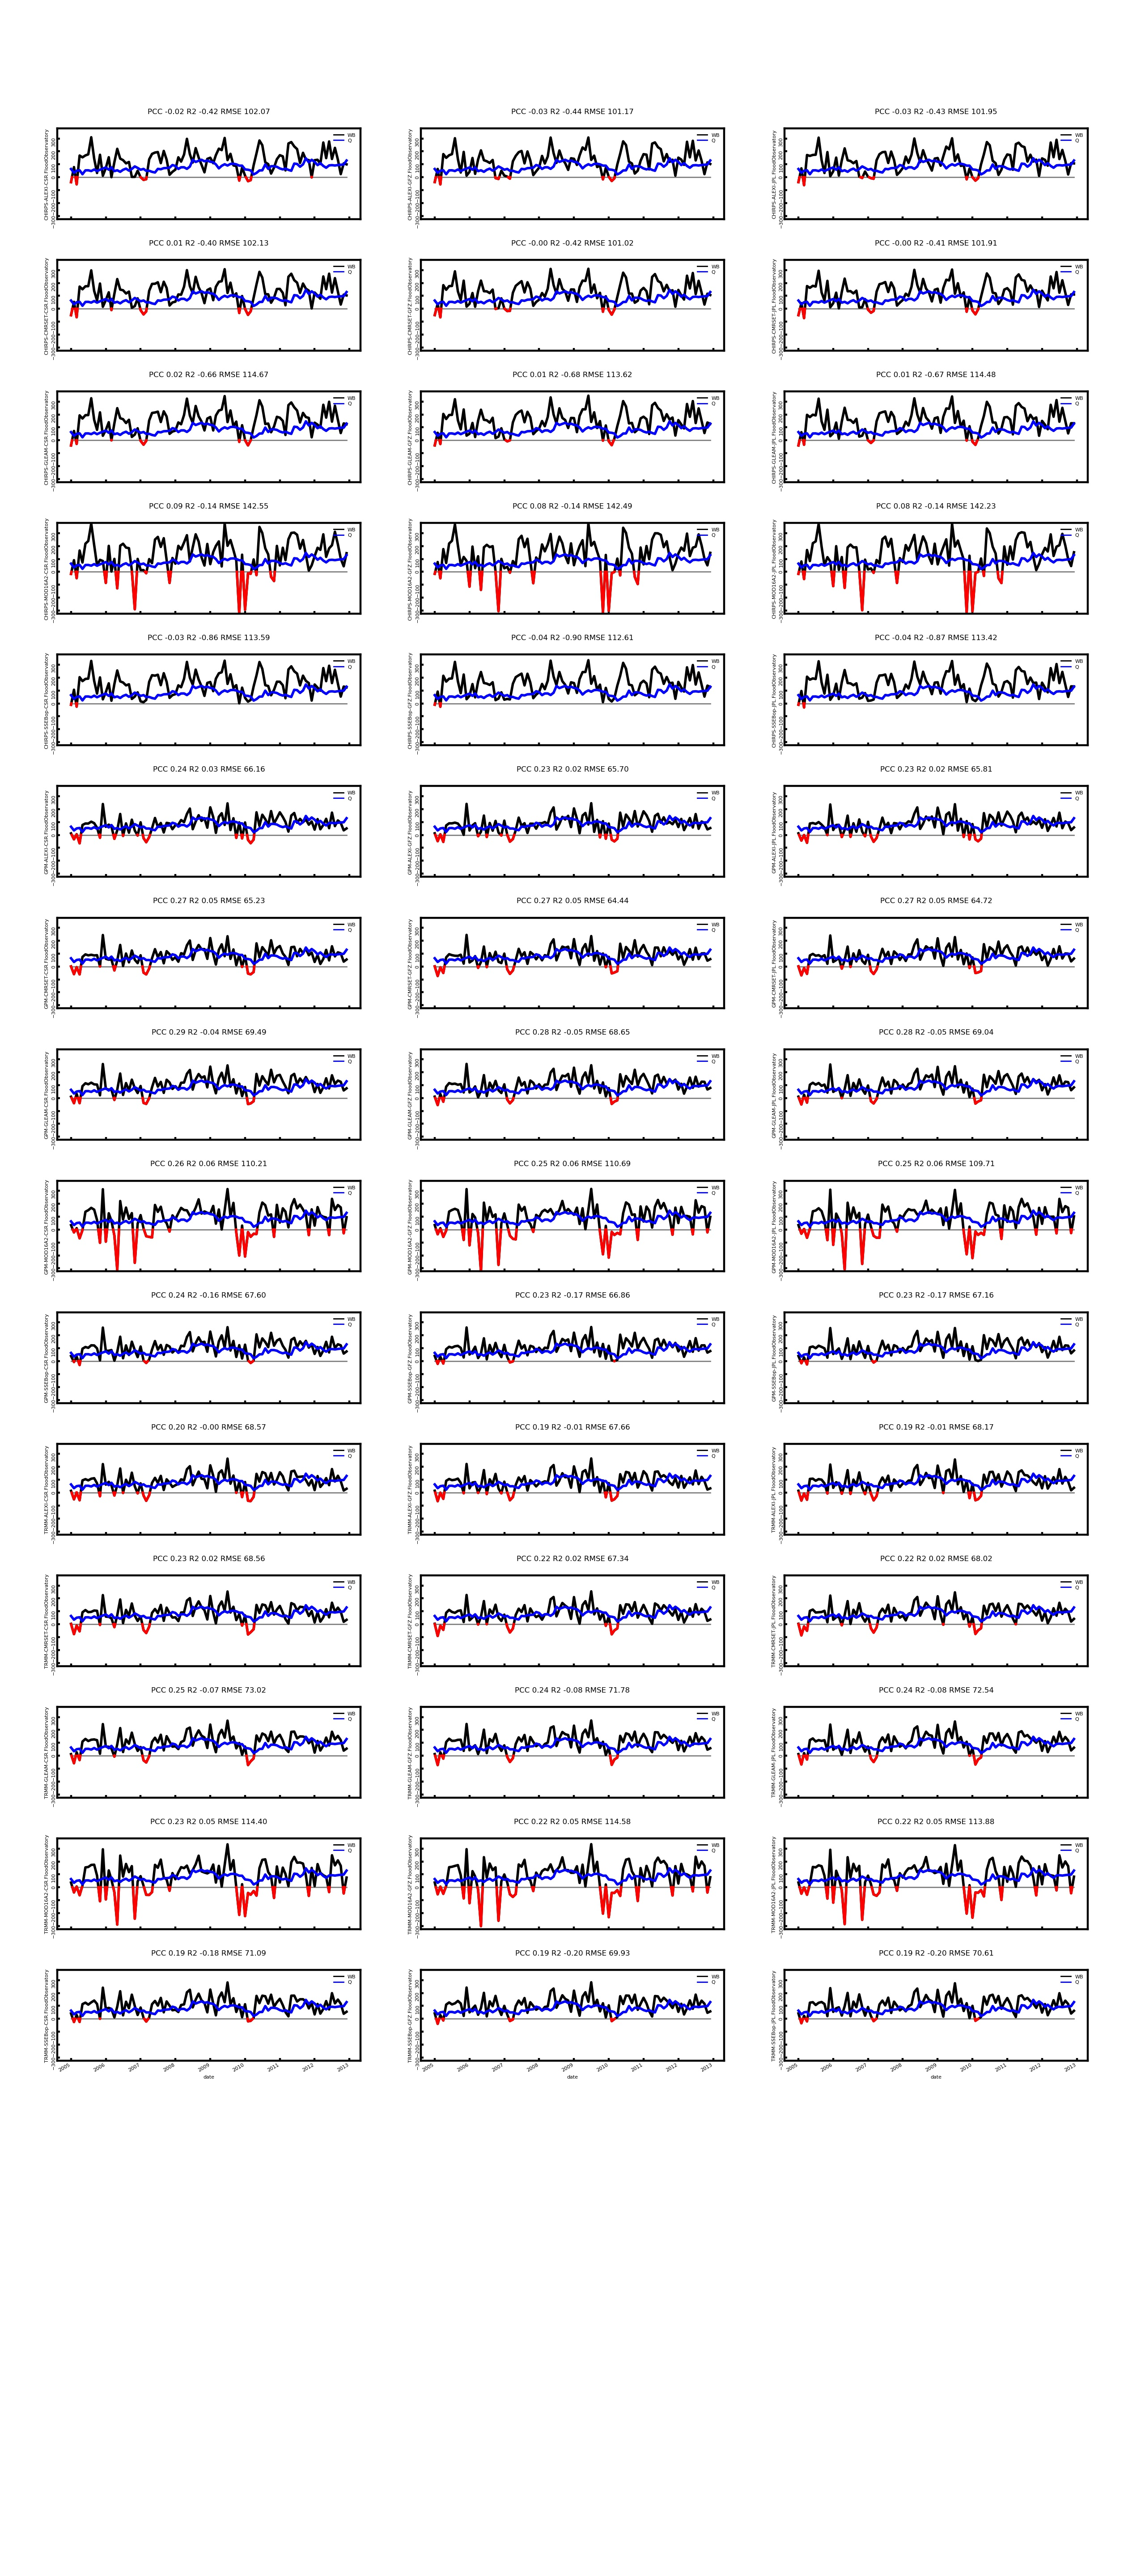
\includegraphics[width=0.8\textwidth]{D:/IHEProjects/TempDev/IHEWAreport/tests/data/area1/fig/fig5.jpg}%
\label{figure:ann1}%
\end{figure}

%
\newpage

%
\cleardoublepage%
\end{document}